\documentclass[11pt]{amsart}
\usepackage[margin=1.15in]{geometry}
\usepackage{amsmath,amssymb,amsthm}
\usepackage{graphicx}
\usepackage{array,longtable}
\usepackage[T1]{fontenc}
\usepackage[utf8]{inputenc}
\usepackage{lmodern}
\usepackage{url}
\usepackage[hidelinks,hypertexnames=false]{hyperref}

\numberwithin{equation}{section}

\theoremstyle{plain}
\newtheorem{theorem}{Theorem}[section]
\newtheorem{proposition}[theorem]{Proposition}
\newtheorem{lemma}[theorem]{Lemma}
\newtheorem{corollary}[theorem]{Corollary}
\newtheorem{lthminner}{Theorem}
\newenvironment{lthm}[1]{\renewcommand\thelthminner{#1}\lthminner}{\endlthminner}
\newtheorem{llemminner}{Lemma}
\newenvironment{llemm}[1]{\renewcommand\thellemminner{#1}\llemminner}{\endllemminner}
\theoremstyle{definition}
\newtheorem{definition}[theorem]{Definition}
\theoremstyle{remark}
\newtheorem{remark}[theorem]{Remark}

\newcommand{\Q}{\mathbb{Q}}
\newcommand{\Z}{\mathbb{Z}}
\newcommand{\R}{\mathbb{R}}
\newcommand{\C}{\mathbb{C}}
\newcommand{\A}{\mathbb{A}}
\newcommand{\Kab}{K^{\mathrm{ab}}}
\newcommand{\Art}{\mathrm{Art}}
\newcommand{\Frob}{\mathrm{Frob}}
\newcommand{\Gal}{\mathrm{Gal}}
\newcommand{\sgn}{\operatorname{sgn}}
\newcommand{\Nm}{\mathrm{Nm}}
\newcommand{\tr}{\operatorname{tr}}

\begin{document}

\title[Reciprocity for quantum dilogarithm values]{A reciprocity law for quantum dilogarithm values at real multiplication points, with applications to Hilbert's twelfth problem, Stark units and SICs}
\author{Imran Zaidi}
\address{Montr\'eal, Qu\'ebec, Canada}
\email{imran.zaidi@gmail.com}
\subjclass[2020]{11R37 (primary); 11R42, 11R27, 11F20, 81P15 (secondary)}
\keywords{Stark units, Hilbert's twelfth problem, quantum dilogarithm, real multiplication, reciprocity law, SIC}
\date{6 October 2026}

\begin{abstract}
Let $K$ be a real quadratic field. Radchenko and Wheeler attached a special value of Faddeev's quantum dilogarithm at a real multiplication point to each triple consisting of a lattice $I\subset K$, a totally positive unit of its multiplier ring and a torsion point of $K/I$, and proved that these values are algebraic. Assuming one of their analytic identities, the Fourier proportionality relation, we prove an idelic reciprocity law for the squared absolute values: they lie in the maximal abelian extension $K^{\mathrm{ab}}$, and every idele of $K$ acts on them through an explicit action on lattices and torsion points, twisted by its sign at the second real place. The proof establishes Frobenius congruences by a $p$-adic argument on the Bruhat--Tits tree and globalizes them with Chebotarev's theorem. With no further analytic input, the values attached to the maximal order are units at every finite prime, and the square roots of all values lie in $K^{\mathrm{ab}}$. Combined with a quadratic relation of Radchenko and Wheeler, the law gives Zauner-symmetric SICs (symmetric informationally complete quantum measurements) in every dimension $M\ge5$. Using Shintani's product formula in Yamamoto's form, we show that the values together with $i$ generate $K^{\mathrm{ab}}$, and we prove the rank-one abelian Stark conjecture at a real place, including Tate's square-root condition, for every abelian extension of $K$ in which that place splits and every set $S$ of places with $|S|\ge3$ containing both real places and the ramified primes. In one configuration the square-root condition also uses the Fourier-transform identity of Faddeev, Kashaev and Volkov; there, using further identities of Radchenko and Wheeler and Shintani's evaluation of cone zeta functions at $s=0$, we prove a stronger root law for the Stark units, unless the trace of the relevant unit $\eta$ is even and $\mathbb Z[\eta]\ne O_K$.
\end{abstract}


\maketitle
\setcounter{tocdepth}{1}
\tableofcontents

\section{Introduction}\label{sec:intro}

Hilbert's twelfth problem asks for explicit generators of the abelian extensions of a number field. For $\mathbb Q$ they are the values of $e^{2\pi ix}$ at rational $x$, and for imaginary quadratic fields they are special values of modular and elliptic functions at CM points. For real quadratic fields, Stark's conjectures predict that suitable units, given by derivatives of $L$-functions at $s=0$, generate abelian extensions, and several authors have proposed analytic functions whose values at real multiplication points should produce these units~\cite{Ko, AFK}. Radchenko and Wheeler~\cite{RW} studied the special values of Faddeev's quantum dilogarithm at real multiplication points, proved that they are algebraic, and established a large system of identities among them. Assuming one of their identities, the Fourier proportionality relation, we prove a reciprocity law for these values and deduce that the values attached to the maximal order are units, that the values generate the maximal abelian extension, and the rank-one abelian Stark conjecture at a real place. With further identities of Radchenko and Wheeler we obtain Tate's square-root condition in all cases and Zauner-symmetric SICs in every dimension $M\ge5$.

\subsection*{Notation}
Let $K\subset\mathbb R$ be a real quadratic field. We call this inclusion the \emph{analytic place}~$r$, write $u$ for the other real place and $\tau$ for the nontrivial automorphism of $K$, and fix $\overline{\mathbb Q}\subset\mathbb C$, so that $\Kab\subset\mathbb C$. Put $\Kab_r:=\Kab\cap\mathbb R$, the maximal abelian extension of $K$ in which $r$ splits completely. For an integral ideal $\mathfrak m\neq O_K$ (a \emph{proper} ideal) let $C_{\mathfrak m}:=\mathrm{Cl}_{\mathfrak m\infty_r\infty_u}(K)$ and $\mathcal G_{\mathfrak m}:=\mathrm{Cl}_{\mathfrak m\infty_u}(K)$, the Galois group of the ray class field $H_{\mathfrak m\infty_u}$, and put $n_{\mathfrak m}:=2/|\ker(C_{\mathfrak m}\to\mathcal G_{\mathfrak m})|\in\{1,2\}$; thus $n_{\mathfrak m}=1$ whenever $K$ has no unit of norm $-1$. The Artin map $\Art_K$ on the ideles $\A_K^\times$ is normalized arithmetically. The idele equal to $-1$ at a real place $v$ and to $1$ elsewhere maps to the complex conjugation $\iota_v$ above $v$, and $c_r,c_u$ denote the corresponding classes.

The values are attached to \emph{data} $d=(I,\varepsilon,z)$: a lattice $I\subset K$ (a $\mathbb Z$-submodule of rank~$2$), with multiplier ring $\mathcal O_I:=\mathrm{End}\,I$ of any conductor; a totally positive unit $\varepsilon\in\mathcal O_I$ with $\varepsilon_r>1$; and $z\in K$ with $(\varepsilon-1)z\in I$ and $z\notin I$, taken modulo $I$. Section~\ref{sec:values} attaches to $d$ a positive number $W(d)$; in the notation of~\cite{RW} it is $|F^+_\gamma(\mathbf u)|^2$, for the matrix $\gamma$ of $\varepsilon$ in a suitable basis of $I$ and the label $\mathbf u$ of $z$. An idele $s\in\A_K^\times$ with finite part $s_f$ acts on data by $s^{-1}d:=(s_f^{-1}I,\varepsilon,s_f^{-1}z)$, where $s_f^{-1}I:=K\cap s_f^{-1}\widehat I$ with $\widehat I:=I\otimes\widehat{\mathbb Z}$, and $s_f^{-1}z$ is read in $K/s_f^{-1}I\cong\A_{K,f}/s_f^{-1}\widehat I$. Let $\mathcal V_K$ be the set of all values $W(d)$, and $\chi_K$ the quadratic character of $K/\mathbb Q$.

The values, the identities they satisfy and their algebraicity are due to Radchenko and Wheeler~\cite{RW}. Our contribution is the reciprocity law and its consequences.

\subsection{Results}\label{sec:results}

Four analytic identities of~\cite{RW} enter as hypotheses, and each theorem below names those it needs: the Fourier proportionality~\cite[(6)]{RW}, which is identity~(vi) of Section~\ref{sec:values}; the five-term relation~\cite[(7)]{RW}, together with its form~\cite[(36)]{RW}, which combines~(7) with~(5); the quadratic relation~\cite[Thm.~7, (39)]{RW}; and the Fourier-transform identity~\cite[(15)]{RW}, which we call~(I1). Radchenko and Wheeler state~(I1) after Faddeev and Kashaev~\cite{FK94}, in the Fourier form of Faddeev, Kashaev and Volkov~\cite{FKV}, at a real point $\tau>0$, together with its continuation. Kopp's limit formula~\cite[Thm.~1.1]{Ko}, a preprint, is used only in the alternative route of Appendix~\ref{app:kopp}. All other inputs are published or classical: Shintani's product formula in Yamamoto's form~\cite{Sh, Ya08, Ya10}, Shintani's evaluation of cone zeta functions at $s=0$~\cite{Sh76}, Rademacher's formula for the eta multiplier~\cite{RG}, Hecke theory, class field theory and Chebotarev's theorem.

\begin{lthm}{A}[Reciprocity law]\label{thm:A}
Assume identity~(6) of~\cite{RW}. Every value $W(d)$ is algebraic and lies in $\Kab$, and for every datum $d$, whatever the multiplier ring of $I$, and every idele $s\in\A_K^\times$,
\begin{equation}\tag{$\star$}\label{eq:star}
\Art_K(s)\,W(d)=W(s^{-1}d)^{\sgn s_u}.
\end{equation}
Equivalently, if $\sigma\in\Gal(\overline{\mathbb Q}/K)$ and $\Art_K(s)=\sigma|_{\Kab}$, then $\sigma W(d)=W(s^{-1}d)^{\sgn s_u}$. Moreover $\overline{\sigma W(d)}=\sigma W(d)^{\chi_K(\sigma)}$ for every $\sigma\in\Gal(\overline{\mathbb Q}/\mathbb Q)$, so the conjugates of $W(d)$ above $r$ are real and those above $u$ lie on the unit circle; the conjugates above $r$ are moreover positive.
\end{lthm}

The restriction of~\eqref{eq:star} to rational ideles reads $\mathrm{Ver}(g)W(I,\varepsilon,z)=W(I,\varepsilon,\chi_{\mathrm{cyc}}(g)z)$ for $g\in\Gal(\mathbb Q^{\mathrm{ab}}/\mathbb Q)$, where $\mathrm{Ver}\colon\Gal(\mathbb Q^{\mathrm{ab}}/\mathbb Q)\to\Gal(\Kab/K)$ is the transfer, which corresponds to the inclusion $\A_{\mathbb Q}^\times\subset\A_K^\times$, and $\chi_{\mathrm{cyc}}$ is the cyclotomic character with values in $\widehat{\mathbb Z}^\times$. This restriction, the unit-circle statement and the positivity above~$r$ are proved without Theorem~\ref{thm:DC} (the $\det=-1$ covariance of Section~\ref{sec:sign}) and without the selection step of Section~\ref{sec:rec}.

Put $f_0:=[O_K:\mathbb Z[\varepsilon]]$ and $\mathfrak M_\varepsilon:=f_0(\varepsilon-1)O_K$. For particular ideles, \eqref{eq:star} specializes as follows.
\begin{center}
\renewcommand{\arraystretch}{1.25}
\begin{tabular}{>{\raggedright\arraybackslash}p{0.36\linewidth}>{\raggedright\arraybackslash}p{0.56\linewidth}}
\hline
idele $s$ & what \eqref{eq:star} says\\
\hline
finite idele of an integral ideal $\mathfrak a$ prime to $\mathfrak M_\varepsilon$ & Artin law $\Art(\mathfrak a)W(I,\varepsilon,z)=W(\mathfrak a_{\mathcal O}^{-1}I,\varepsilon,z)$, $\mathfrak a_{\mathcal O}:=\mathfrak a\cap\mathcal O_I$, for every order\\
$-1$ at $r$ & the values are real at $r$\\
$-1$ at $u$ & $\iota_uW=W^{-1}$\\
$\alpha\in K^\times$ & homothety law $W(\alpha^{-1}I,\varepsilon,\alpha^{-1}z)=W(I,\varepsilon,z)^{\sgn\alpha_u}$, so the right side of \eqref{eq:star} is $K^\times$-invariant\\
$a\in\widehat{\mathbb Z}^\times$ & scaling of labels, $W(I,\varepsilon,a^{-1}z)$\\
\hline
\end{tabular}
\end{center}

For a proper $\mathfrak m$ let $\varepsilon_{\mathfrak m}>1$ generate the totally positive units $\equiv1\pmod{\mathfrak m}$, and put $\mathbf W_{\mathfrak m}:=W(\mathfrak m,\varepsilon_{\mathfrak m},1)$. The maximal-order values with annihilator $\mathfrak m$ form a function $W_{\mathfrak m}$ on $\mathcal G_{\mathfrak m}$ with $W_{\mathfrak m}(1)=\mathbf W_{\mathfrak m}$ (Section~\ref{sec:h12}). We shall need the following nonvanishing property: for every proper $\mathfrak f$ and every primitive character $\chi$ of $\mathcal G_{\mathfrak f}$ with $\chi(c_u)=-1$,
\begin{equation}\tag{N}\label{eq:N}
\sum_{B\in\mathcal G_{\mathfrak f}}\bar\chi(B)\log W_{\mathfrak f}(B)\neq0.
\end{equation}

\begin{lthm}{B}[Hilbert's twelfth problem for $K$]\label{thm:B}
Assume identity~(6) of~\cite{RW}. Then $K(\mathcal V_K)=\Kab_r$ and $\Kab=K(i,\mathcal V_K)$; already the values $\mathbf W_{\mathfrak m}$, $\mathfrak m$ proper, generate $\Kab_r$.
\end{lthm}

The proof uses~\eqref{eq:N}, which we prove in Proposition~\ref{prop:N} from Shintani's product formula in Yamamoto's form~\cite[Prop.~3]{Sh}, \cite[Thm.~5.1.1]{Ya08}, together with Yamamoto's relation for the class $c_u$~\cite[Thm.~5.2.3]{Ya08} and Hecke theory. Appendix~\ref{app:kopp} derives~\eqref{eq:N} also from Kopp's limit formula.

\begin{lthm}{C}[Zauner SICs]\label{thm:C}
Assume identity~(6) of~\cite{RW} and the quadratic relation~\cite[Thm.~7, (39)]{RW}. For every $M\ge5$ there is a Weyl--Heisenberg SIC in dimension $M$ whose fiducial vector is fixed, up to phase, by an order-three Clifford unitary whose symplectic part is $\mathrm{SL}_2(\mathbb Z)$-conjugate to Zauner's matrix $F_Z^{\pm1}$.
\end{lthm}

\begin{lthm}{D}[Units at every finite prime]\label{thm:D}
Assume identity~(6) of~\cite{RW}. For every invertible $O_K$-ideal $I$, every totally positive $\varepsilon\in O_K^\times$ with $\varepsilon_r>1$ and every $z$ as above, $W(I,\varepsilon,z)$ and the corresponding value $E_\gamma(z/v_2)$ of~\cite{RW} (Section~\ref{sec:values}) are units at every finite prime of every number field containing them.
\end{lthm}

\begin{lthm}{E}[Square roots]\label{thm:G}
Assume identity~(6) of~\cite{RW}. For every datum $d$, whatever the multiplier ring of $I$, $\sqrt{W(d)}\in\Kab$.
\end{lthm}

For the Stark statements put $Z_{\mathfrak m}(s,B):=\zeta_{\mathfrak m}(s,B)-\zeta_{\mathfrak m}(s,c_uB)$ for $B\in\mathcal G_{\mathfrak m}$, where $\zeta_{\mathfrak m}(s,B)$ is the partial zeta function of $B$. The \emph{analytic dictionary} is the statement that for every proper $\mathfrak m$ and every $B\in\mathcal G_{\mathfrak m}$
\begin{equation}\tag{V}\label{eq:V}
\log W_{\mathfrak m}(B)=-n_{\mathfrak m}\,Z'_{\mathfrak m}(0,B).
\end{equation}
We prove~\eqref{eq:V} from Shintani's product formula in Yamamoto's form (Theorem~\ref{thm:dict}). Appendix~\ref{app:kopp} derives it also from Kopp's limit formula~\cite[Thm.~1.1]{Ko}; the two routes share only Shintani's work and Hecke theory.

Let $H/K$ be a finite abelian extension in which $r$ splits completely, and $S$ a set of places of $K$ containing $r$, $u$ and the primes ramified in $H/K$, with $|S|\ge3$. Put $\mathfrak m:=\mathfrak f(H/K)\prod_{\mathfrak q\in S\text{ finite}}\mathfrak q$. Let $\zeta_S(s,\sigma)$ be the partial zeta function of $\sigma\in\Gal(H/K)$ with the Euler factors at the finite places of $S$ removed, and $w_r$ a fixed place of $H$ above $r$. The rank-one abelian Stark conjecture $\mathrm{St}(H/K,S)$, in Tate's formulation~\cite[Ch.~IV]{Ta} (see also~\cite{Ru}), predicts an element $\varepsilon_H\in H^\times$ with
\begin{itemize}
\item[(St1)] $|\varepsilon_H|_w=1$ for every place $w$ of $H$ not above $r$;
\item[(St2)] $\log|\varepsilon_H^\sigma|_{w_r}=-2\zeta_S'(0,\sigma)$ for all $\sigma\in\Gal(H/K)$;
\item[(St3)] $H(\sqrt{\varepsilon_H})/K$ is abelian.
\end{itemize}
Call a modulus $\mathfrak m'$ \emph{$S$-adapted} if its support is the set $S_f$ of finite places of $S$ and $\mathfrak f(H/K)\mid\mathfrak m'$. If every $S$-adapted $\mathfrak m'$ has $n_{\mathfrak m'}=2$ and $S$ contains no prime above~$2$, we say that $(H,S)$ is in the \emph{open configuration}. Otherwise some $S$-adapted $\mathfrak m'$ has $n_{\mathfrak m'}=1$; this is always the case if $K$ has no unit of norm $-1$ or if $S$ contains a prime above~$2$.

\begin{lthm}{F}[Rank-one abelian Stark conjecture at a real place]\label{thm:E}
Assume identity~(6) of~\cite{RW}, and, if $(H,S)$ is in the open configuration, also~(I1). Then $\mathrm{St}(H/K,S)$ holds for every pair $(H,S)$ as above: there is $\varepsilon_H$ satisfying (St1), (St2) and (St3).
\end{lthm}

The proof uses~\eqref{eq:V}.

In the open configuration let $\eta$ be the generator of the units $\equiv1\pmod{\mathfrak m}$ with signs $(-,+)$ at $(r,u)$, so that $\Nm\eta=-1$ and $\varepsilon_{\mathfrak m}=\eta^2$. For $A\in\mathcal G_{\mathfrak m}$ put $U_A:=\exp(-Z'_{\mathfrak m}(0,A))$; these are the Stark units, and $U_A=+\sqrt{W_{\mathfrak m}(A)}$. In this configuration we take $H:=H_{\mathfrak m\infty_u}$, and put $t:=|\tr\eta|\ge3$ and $f_\eta:=[O_K:\mathbb Z[\eta]]$.

\begin{lthm}{G}[Root law]\label{thm:F}
Assume identity~(6) of~\cite{RW} and~(I1). In the open configuration, $-\eta U_A\in H^{\times2}$ for every class $A$ in each of the following cases:
\begin{enumerate}
\item[(a)] $t$ odd (then $2$ is inert in $K$), for every $f_\eta$ and every class number of $H$, assuming in addition~\cite[(7)]{RW} at three families of pairs of labels (Section~\ref{sec:rootlaw});
\item[(b)] $f_\eta=1$, that is $O_K=\mathbb Z[\eta]$, for every $t$, assuming in addition~\cite[(36)]{RW} at one family of pairs of labels, the slice $\{2c\}\times B$ of Section~\ref{sec:rootlaw}.
\end{enumerate}
\end{lthm}

In both cases the proof of Theorem~\ref{thm:F} uses~\eqref{eq:V}, Shintani's evaluation of two-dimensional cone zeta functions at $s=0$~\cite{Sh76} (through Theorem~\ref{thm:phase}) and Rademacher's formula. The root law for $t$ even and $f_\eta>1$ remains open. We have checked it in about $130$ cases of the open configuration over some $25$ fields, exactly once the Stark units are recognized as roots of explicit polynomials. The cases include $2$ inert, split and ramified, and $t$ even; there was no failure.

Along the way we prove an archimedean sign law for the values (Theorem~\ref{thm:sign}) and a formula for their phases (Theorem~\ref{thm:phase}). The deduction of Theorem~\ref{thm:B} from Theorem~\ref{thm:A} and~\eqref{eq:N} follows the classical pattern of~\cite[Ch.~IV]{Ta} and~\cite{St} (compare~\cite{Ro}); we claim no novelty for it. Through~\eqref{eq:V}, Theorem~\ref{thm:A} is the reciprocity part of Stark's conjecture for the numbers $\exp(-n_{\mathfrak m}Z'_{\mathfrak m}(0,B))$.

\subsection{Relation to other work}\label{sec:other}

Hilbert's twelfth problem for totally real fields has a $p$-adic solution: Dasgupta and Kakde show that Brumer--Stark units, given by an exact $p$-adic formula~\cite{DK1}, together with $n-1$ easily described elements generate the maximal abelian extension of a totally real field of degree~$n$~\cite{DK2}. For real quadratic fields, Darmon and Vonk proposed $p$-adic singular moduli~\cite{DV}, and Darmon, Pozzi and Vonk proved that the values of the Dedekind--Rademacher cocycle at real multiplication points are $p$-units in the narrow Hilbert class field~\cite{DPV}.

The present work is archimedean: the generators are values of one complex-analytic function at real multiplication points, conjectured to be Stark units at a real place~\cite{Ko, RW}. Radchenko and Wheeler prove that these values are algebraic~\cite[Thm.~1]{RW} through an overdetermined system of polynomial equations. The reciprocity law uses one equation of that system,~\cite[(6)]{RW}, and recovers algebraicity (Proposition~\ref{prop:alg}). All analytic input to the reciprocity law is in that identity, proved in~\cite{RW}; the arithmetic part is a $p$-adic argument (Section~\ref{sec:local}) that turns the identity into Frobenius congruences. The archimedean rank-one Stark conjecture for real quadratic fields is stated as open in~\cite[\S1.5]{Ko} and~\cite[\S1]{RW}; Kopp obtains the unit property under a further hypothesis:~\cite[Thm.~1.3(2)]{Ko} assumes~\cite[Conj.~6.9]{Ko}.

Kopp asks in~\cite[\S1.5]{Ko} for an analogue of Shimura's reciprocity law for the real multiplication values of his Shintani--Faddeev cocycle, and notes that for their squares, in the fundamental-discriminant case, such a law would follow from the Stark conjectures. For maximal-order data $W(d)^{-1}$ is a power of $|\mathrm{Sh}^{\mathbf r}_A(\beta)|^2=\exp(n_{\mathfrak m}Z'_{\mathfrak m}(0,\mathfrak A))$, the modulus in~\cite[Thm.~1.1]{Ko} (Appendix~\ref{app:kopp}), so Theorem~\ref{thm:A} gives such a law for these numbers without assuming the Stark conjectures. We do not relate the values at non-maximal orders to Kopp's. The shape of~\eqref{eq:star} resembles Shimura's reciprocity law for CM torsion values~\cite[Ch.~5]{Shi}, with the archimedean component acting through $\sgn s_u$; we use this only as an analogy.

Zauner conjectured the existence of SICs with his symmetry in every dimension~\cite{Za}. Appleby, Flammia and Kopp proposed a construction through Stark units~\cite{AFK}, and Radchenko and Wheeler proved, for their values, the quadratic relation on which it rests~\cite[\S4.4, Thm.~7]{RW}. Theorem~\ref{thm:C} supplies the remaining step: a Galois conjugate of the values of modulus one. Radchenko and Wheeler obtain these conjugates independently in~\cite{RW2}.

While this paper was in preparation, Radchenko and Wheeler released a preprint~\cite{RW2} in which they prove, with a different local argument based on the five-term relation~\cite[(7)]{RW}, that all the values are units and satisfy an Artin reciprocity law, and deduce Stark's reciprocity, the generation of the ray class fields and the unitary conjugates needed for Zauner's conjecture. On 29 September 2026 we sent them an account of an integrality argument at inert primes, the resulting Frobenius congruences and their application to SICs in even dimensions, and on 30 September an outline of exact root extraction and of a Chebotarev argument placing a Galois conjugate of the values on the unit circle.

\subsection{Outline of the proof}\label{sec:arch}

Frobenius at a split prime $p=\mathfrak p\bar{\mathfrak p}$ is visible in the residues of the values. Radchenko and Wheeler's line product formula, combined with power inheritance, writes $W(\mathfrak p^{-1}I,z)$, the value of a lattice one step away, as an exact product of $W(I,z)$ and values of $I$ for the power $\varepsilon^{k_0}$ along a line $T_{\mathfrak p}$ of labels, where $k_0$ is the order of $\varepsilon$ modulo $\mathfrak p$; the $k_0$-th root is extracted exactly (Section~\ref{sec:root}). If the residues modulo a prime $\mathfrak P\mid\mathfrak p$ are constant along that line, the product collapses to
\[
W(I,z)^p\equiv W(\mathfrak p^{-1}I,z)\pmod{\mathfrak P},
\]
which is what a reciprocity law predicts for $\Frob_{\mathfrak p}$ acting by $I\mapsto\mathfrak p^{-1}I$. The proof establishes this congruence, a statement about the $p$-adic rigidity of the values, and then globalizes it. Figure~\ref{fig:deps} shows the dependencies.

\emph{The local theorem} (Section~\ref{sec:local}). Identity~(6) of~\cite{RW}, with the line product formula and reflection, implies that at all but finitely many primes $p\ge5$ unramified in $K$ every value is a $p$-adic unit, and that for split $p$ the residues are constant along $T_{\mathfrak p}$ or along $T_{\bar{\mathfrak p}}$. The matrices linked by the line product formula fill a region of bounded height in the Bruhat--Tits tree (the tube lemma). An exact multiplicative identity, the \emph{defect identity}, makes a defect valuation an average over the next layer outward. Identity~(6), through an integrality bound of degree $\lfloor p/3\rfloor$ on the outermost layer (a \emph{code bound}), turns a pole there into a larger pole one step inward. Together these exclude a pole of maximal order.

\emph{Exact root extraction} (Section~\ref{sec:root}). The family is built from a power $\gamma^{k_0}$, and a congruence between $k_0$-th powers would lose a root of unity. The root is therefore taken among positive reals, before reduction, through an exact orbit-product identity. This gives the \emph{Frobenius congruence} with two candidates, $\mathfrak p$ and $\bar{\mathfrak p}$; nothing local chooses between them.

\emph{Chebotarev and selection} (Section~\ref{sec:rec}). Chebotarev's theorem turns the congruences into exact statements about Galois elements, still with two candidates. The choice is forced by two global symmetries: reality at the analytic place~$r$, and the homothety law, whose negative-norm case is a new identity (Theorem~\ref{thm:DC}). This proves Theorem~\ref{thm:A}.

The other theorems of Part~A follow quickly. Theorem~\ref{thm:D} combines Theorem~\ref{thm:A} at the bad primes with the local argument. Theorem~\ref{thm:C} needs one Galois conjugate of the values on the unit circle, which the Galois form of Theorem~\ref{thm:A} supplies, and Radchenko and Wheeler's quadratic relation. Theorem~\ref{thm:B} needs in addition the nonvanishing property~\eqref{eq:N}. Theorem~\ref{thm:G} comes from the same local machinery at a second family of primes.

\emph{Part~B} (Section~\ref{sec:partB}). The dictionary~\eqref{eq:V} makes the values Stark units and gives (St1), (St2) and, when $n_{\mathfrak m}=1$, (St3). When $n_{\mathfrak m}=2$ the Stark units are square roots of values, and Theorem~\ref{thm:sqrtrec} gives their own reciprocity law. In the open configuration (St3) follows (Theorem~\ref{thm:st3}) from an identity on the lattice $\mathbb Z[\eta]$ (Theorem~\ref{thm:W}), which we derive by Radchenko and Wheeler's contour method from the Fourier-transform identity of Faddeev, Kashaev and Volkov. Theorem~\ref{thm:F} sharpens (St3) to the root law, through a dyadic computation for $t$ odd and through Theorem~\ref{thm:W} on $O_K$ when $O_K=\mathbb Z[\eta]$.

\begin{figure}[t]
\centering
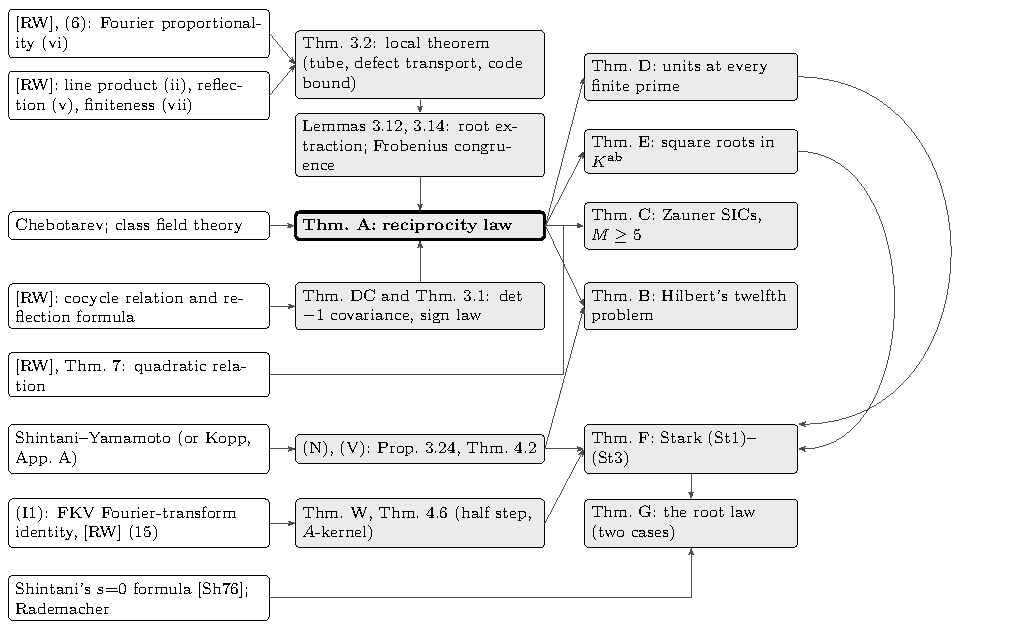
\includegraphics[width=\linewidth]{deps}
\caption{Dependencies among the main results. Boxes on the left are imported results, boxes in the middle are the new arguments, and boxes on the right are the main theorems. Theorem~\ref{thm:F} also uses further identities of~\cite{RW} (Section~\ref{sec:rootlaw}).}
\label{fig:deps}
\end{figure}

No Stark conjecture, no Shimura reciprocity and no moduli interpretation of real multiplication points enter the proof of Theorem~\ref{thm:A}, and the values are never assumed to be algebraic or integral. Section~\ref{sec:inputs} lists what is new and what is imported.

Section~\ref{sec:values} defines the values and lists the identities we use. Section~\ref{sec:partA} proves Theorems~\ref{thm:A}--\ref{thm:G}, and Section~\ref{sec:partB} proves Theorems~\ref{thm:E} and~\ref{thm:F}. Section~\ref{sec:inputs} lists the imported results and what each theorem depends on, and Section~\ref{sec:verif} describes how the argument has been checked. This work was carried out with substantial assistance from AI systems, and all review of it so far has been by AI agents (Section~\ref{sec:verif}).

\section{The values and the identities they satisfy}\label{sec:values}

We define the positive numbers \(W(d)\) and list the identities they satisfy. Identities (i)--(vii) are results of Radchenko and Wheeler~\cite{RW}; (ix) follows from~\cite[(3)]{RW}; (viii) and (x) are ours and are proved in Section~\ref{sec:sign}.

\subsubsection*{Faddeev's modular quantum dilogarithm}
Write \(e(x):=e^{2\pi ix}\) and \(j(g,\tau):=c_g\tau+d_g\) for \(g=\bigl(\begin{smallmatrix}a_g&b_g\\c_g&d_g\end{smallmatrix}\bigr)\). In this section, and in the analytic formulas of Sections~\ref{sec:dict} and~\ref{sec:open}, \(\tau\) denotes a complex variable, not the automorphism of \(K\). For \(\gamma\in\mathrm{SL}_2(\mathbb Z)\), \(m,n\in\mathbb Z\) and \((z,\tau)\in\mathbb C\times(\mathbb C\smallsetminus\mathbb R)\), Radchenko and Wheeler~\cite[(1)]{RW}, following Garoufalidis, Kashaev and Zagier~\cite{GKZ}, put
\[\Phi_{\gamma,m,n}(z;\tau):=\frac{(q^me(z);q)_\infty}{(\tilde q^{\,n}e(z/j(\gamma,\tau));\tilde q)_\infty},\qquad q=q_\tau:=e(\tau),\quad \tilde q=\tilde q_\tau:=e(\gamma\tau).\]
For \(S=\bigl(\begin{smallmatrix}0&-1\\1&0\end{smallmatrix}\bigr)\) one has \(\Phi_{S,m,n}(z;\tau)=\Phi_S(z+m\tau-n;\tau)\) with \(\Phi_S:=\Phi_{S,0,0}\), and for \(\tau>0\) (after continuation) this is Faddeev's quantum dilogarithm:
\[\Phi_S(z;\tau)=\varphi_{\mathsf b}\bigl(i\mathsf b^{-1}z-i\mathsf b/2+i/(2\mathsf b)\bigr),\qquad \mathsf b=\sqrt\tau,\]
where \(\log\varphi_{\mathsf b}(x)=\int_{\mathbb R+i0}e^{-2ixw}\,dw/(4w\sinh(\mathsf bw)\sinh(w/\mathsf b))\).
By~\cite[Prop.~2(i)]{RW}, \(\Phi_{\gamma,m,n}\) is a finite product of factors \(\Phi_S(z+(m+\ell)\tau+k_\ell;\,j(\gamma,\tau))\), so it continues meromorphically to \(j(\gamma,\tau)\notin\mathbb R_{\le0}\), in particular to a real fixed point of \(\gamma\). The \emph{index rules}
\[\Phi_{\gamma,m,n}=(1-q^me(z))\,\Phi_{\gamma,m+1,n},\qquad \Phi_{\gamma,m,n+1}=(1-\tilde q^{\,n}e(z/j(\gamma,\tau)))\,\Phi_{\gamma,m,n}\]
follow from the definition and \((x;q)_\infty=(1-x)(qx;q)_\infty\). Two functional equations of~\cite{RW} are used directly: the \emph{cocycle relation}~\cite[(17)]{RW},
\[\Phi_{gh,m,n}(z;\tau)=\Phi_{g,k,n}\bigl(z/j(h,\tau);\,h\tau\bigr)\,\Phi_{h,m,k}(z;\tau)\qquad(k\in\mathbb Z),\]
and the \emph{reflection formula}~\cite[\S2.2]{RW}
\[\Phi_{\delta g\delta,1-m,1-n}(z;-\tau)=\Phi_{g,m,n}(z;\tau)^{-1},\qquad \delta:=\mathrm{diag}(1,-1).\]
Both hold on \(\mathbb C\times(\mathbb C\smallsetminus\mathbb R)\), and they extend to the real point because the domain of meromorphy is connected.

\subsubsection*{Admissible matrices and labels}
Call \(\gamma=\bigl(\begin{smallmatrix}a&b\\c&d\end{smallmatrix}\bigr)\in\mathrm{SL}_2(\mathbb Z)\) \emph{admissible} if it is hyperbolic with \(c>0\) and \(\operatorname{tr}\gamma\ge3\). Let \(\tau^*\) be its attracting fixed point. Then \(\varepsilon_\gamma:=c\tau^*+d>1\) is a totally positive unit of norm \(1\) in \(K=\mathbb Q(\tau^*)\), and \(\gamma(\tau^*,1)^{\mathsf T}=\varepsilon_\gamma(\tau^*,1)^{\mathsf T}\). Put \(I_\gamma:=\mathbb Z\tau^*+\mathbb Z\), \(t_\varepsilon:=\varepsilon_\gamma^{-1}-1\) and
\[G_\gamma:=t_\varepsilon^{-1}I_\gamma/I_\gamma\;\cong\;\mathbb Z^2/\Lambda_\gamma,\qquad\Lambda_\gamma:=\mathbb Z^2(\gamma-I),\]
where \(x\in t_\varepsilon^{-1}I_\gamma\) has \emph{label} \(\mathbf u\in\mathbb Z^2\) (a row vector) defined by \((\varepsilon_\gamma^{-1}-1)x=u_1\tau^*+u_2\). The group \(G_\gamma\) has order \(N_\gamma=\operatorname{tr}\gamma-2\), and \(\varepsilon_\gamma\) fixes it pointwise.

\subsubsection*{The values of Radchenko and Wheeler}
For \(\mathbf u\notin\Lambda_\gamma\) put
\[E_\gamma(\mathbf u):=\mu_\gamma\,\Phi_{\gamma,u_1,0}\Bigl(\frac{u_1\tau^*+u_2}{\varepsilon_\gamma^{-1}-1};\,\tau^*\Bigr),\qquad E_\gamma(0):=\varepsilon_\gamma^{1/2},\]
where \(\mu_\gamma\in\mu_{24}\) is the multiplier of Dedekind's eta function, \(\eta(\gamma w)=\mu_\gamma\sqrt{cw+d}\,\eta(w)\). This is \(F^+_\gamma(\mathbf u)\) of~\cite[(2), (4)]{RW}, evaluated at the attracting point as in~\cite[(37)]{RW}. The first argument is the torsion point of label \(\mathbf u\), so \(E_\gamma\) is a function on \(G_\gamma\). We call a pair \((m,n)\) of integers with \(m-n=u_1\) \emph{compatible} with the label \(\mathbf u\). At a fixed point, the index quasi-periodicity~\cite[(16)]{RW} gives \(\Phi_{\gamma,m,n}=\Phi_{\gamma,u_1,0}\) at the torsion point of label \(\mathbf u\) for every compatible pair; the intermediate factors \(1-e(\cdot)\) are nonzero because the point does not lie in the lattice.

The Gaussian and its bicharacter are~\cite[(3)]{RW}
\[q(\mathbf u):=(-1)^{u_1+u_2+u_1u_2}e_{2N}\bigl(\omega(\mathbf u\gamma,\mathbf u)\bigr),\qquad b(\mathbf u,\mathbf v):=e_N\bigl(\omega(\mathbf u\gamma-\mathbf u,\mathbf v)\bigr),\]
with \(\omega(\mathbf v,\mathbf w)=v_1w_2-v_2w_1\), \(e_N(x)=e(x/N)\) and \(N=N_\gamma\). Both are \(\Lambda_\gamma\)-periodic. The Gaussian \(q\), not to be confused with the nome \(q_\tau\), is even, \(b(x,x)=q(x)^2\), \(q(nx)=q(x)^{n^2}\), and \(q\) takes values in \(\mu_{2e}\), where \(e\) is the exponent of \(G_\gamma\). Write \((\mathcal Ff)(y):=N^{-1/2}\sum_{x}b(x,y)f(x)\) and, for \(x\ne0\), \(w_\gamma(x):=q(x)E_\gamma(x)^2\).

\subsubsection*{The values \(W(d)\)}
Let \(d=(I,\varepsilon,z)\) be a datum (Section~\ref{sec:intro}). A basis \((v_1,v_2)\) of \(I\) is a \emph{fixed frame} if \(v_2\) is totally positive and \(\theta:=v_1/v_2\) satisfies \(\theta_r>\theta_u\). Fixed frames exist: take \(v_2\) to be the positive generator of \(I\cap\mathbb Q\) and adjust the sign of \(v_1\). The matrix \(\gamma\) of \(\varepsilon\) in a fixed frame, \(\varepsilon(\theta,1)^{\mathsf T}=\gamma(\theta,1)^{\mathsf T}\), is admissible, since \(c(\theta_r-\theta_u)=\varepsilon_r-\varepsilon_u>0\); moreover \(\tau^*=\theta_r\), \(\varepsilon_\gamma=\varepsilon\) and \(I_\gamma=v_2^{-1}I\). Put
\[W(d)=W(I,\varepsilon,z):=w_\gamma(z/v_2),\]
reading \(z/v_2\) as a nonzero label of \(G_\gamma\). Two fixed frames differ by some \(g\in\mathrm{SL}_2(\mathbb Z)\) with \(j(g,\theta)=v_2'/v_2\gg0\), so (vii) below makes \(W\) independent of the frame, and (iv) makes it a positive real. The value \(W\) is unchanged under \((I,z)\mapsto(\beta I,\beta z)\) for \(\beta\gg0\); also \(w_\gamma(x)=W(I_\gamma,\varepsilon_\gamma,x)\), and \(W(I,\varepsilon^k,z)=W(I,\varepsilon,z)^k\) by (iii). When \(\varepsilon\) is fixed we write \(W(I,z)\).

\subsubsection*{The identities}
The following hold for every admissible \(\gamma\), with no restriction on \(N\); we write \(E=E_\gamma\), \(G=G_\gamma\) and \(N=N_\gamma\).
\begin{enumerate}
\item[(i)] \emph{Regularity.} \(E\) is regular at the real multiplication point and nowhere zero on \(G\); \(E(0)=\varepsilon^{1/2}\).
\item[(ii)] \emph{Line product formula.} For a subgroup \(T\subset G\) of prime order \(p\) there are an admissible \emph{sibling} \(\gamma_T\) of the same trace, with lattice \(I_\gamma+\widetilde T\) (where \(\widetilde T\) is the preimage of \(T\)), and a projection \(\pi_T:G\to G_{\gamma_T}\) with kernel \(T\), such that
\[\prod_{h\in T}E(y+h)=\kappa_T\,E_{\gamma_T}(\pi_Ty)\]
for every coset \(y+T\), with \(\kappa_T=\mu_\gamma^p/\mu_{\gamma_T}\in\mu_{24}\) independent of the coset, the origin coset included.
\item[(iii)] \emph{Power inheritance.} \(E_{\gamma^k}=E_\gamma^k\) and \(q_{\gamma^k}=q_\gamma^k\) on \(G_\gamma\subset G_{\gamma^k}\).
\item[(iv)] \emph{Real type.} \(\overline{E(x)}=q(x)E(x)\); hence \(w_\gamma(x)=|E(x)|^2>0\).
\item[(v)] \emph{Reflection.} \(E(x)E(-x)=q(x)^{-1}\) for \(x\ne0\); hence \(w_\gamma(-x)=w_\gamma(x)^{-1}\).
\item[(vi)] \emph{Fourier proportionality.} \(\mathcal FE(y)=\lambda\,q(y)E(-y)\) for all \(y\), the origin included. Only the existence of some scalar \(\lambda\) is used. Completing the square gives \((q^{-1}\mathcal F^{-1})^3=\gamma_G\cdot I\) with \(\gamma_G=N^{-1/2}\sum_yq(y)^{-1}\in\mu_8\) (Milgram's formula,~\cite[Appendix~4]{MH}), so (vi) alone forces \(\lambda^3=\gamma_G\) and \(\lambda\in\mu_{24}\). Radchenko and Wheeler show that \(\lambda=\mu_\gamma\); this is used only for the root law, Section~\ref{sec:rootlaw}.
\item[(vii)] \emph{Covariance, finiteness, \(\varepsilon\)-invariance.} If \(g\in\mathrm{SL}_2(\mathbb Z)\), \(j(g,\tau^*)>0\) and \(\gamma'=g\gamma g^{-1}\) is admissible, then \(E_{\gamma'}(\mathbf ug^{-1})=(\mu_{\gamma'}/\mu_\gamma)E_\gamma(\mathbf u)\). The values of all admissible matrices of a given trace form a finite set. Finally, \(E_{\gamma^k}(\mathbf u\gamma)=E_{\gamma^k}(\mathbf u)\) on \(G_{\gamma^k}\).
\item[(viii)] \emph{Homothety law.} \(W(\beta I,\varepsilon,\beta z)=W(I,\varepsilon,z)^{\operatorname{sgn}\beta_u}\) for \(\beta\in K^\times\).
\item[(ix)] \emph{Gaussian under odd changes.} For a sibling along \(T\) of odd prime order \(p\), with row-label map \(M_T\) (so \(\gamma M_T=M_T\gamma_T\) and \(\det M_T=p\)), one has \(q_{\gamma_T}(xM_T)=q_\gamma(x)^p\); for \(\pi\in\mathbb Z[\varepsilon]\) of odd norm, \(q(\pi x)=q(x)^{\mathrm{Nm}\,\pi}\). Both statements follow from~\cite[(3)]{RW} and \(q(nx)=q(x)^{n^2}\). At \(p=2\), or for even norm, a sign \(-1\) can appear; those cases are not used.
\item[(x)] \emph{Covariance under determinant \(-1\)} (Theorem~\ref{thm:DC} in Section~\ref{sec:sign}): the analogue of (vii) for \(\det g=-1\) and \(j(g,\tau^*)<0\), with complex conjugation.
\end{enumerate}

\subsubsection*{Sources}
For (i): by~\cite[\S2]{RW} (from~\cite[Prop.~2]{RW}), the zeros and poles of \(\Phi_{\gamma,m,n}(\cdot;\tau^*)\) lie in \(\mathbb Z\tau^*+\mathbb Z=I_\gamma\), which the torsion points avoid, and \(E_\gamma(0)=\varepsilon^{1/2}\) is their convention~\cite[(4), (37)]{RW}; that \(E_\gamma\) is a function on \(G_\gamma\) is~\cite[Lemma~2]{RW}. Identity (ii) is~\cite[Prop.~9, (29)]{RW}; (iii) and the \(\varepsilon\)-invariance in (vii) are~\cite[Prop.~8]{RW}; (iv) is~\cite[Prop.~7 and Cor.~1]{RW}; (v) is~\cite[(5)]{RW} (from~\cite[Prop.~1]{RW}); (vi) is~\cite[Thm.~2, (6)]{RW} together with~\cite[(5)]{RW}, transported to the attracting point by Lemma~\ref{lem:FX} below; the covariance in (vii) follows from~\cite[(17)]{RW}; and (ix) follows from~\cite[(3)]{RW}. As a check of Radchenko and Wheeler's results we have re-derived (i)--(v), (vii) and (ix) from their definitions~\cite[(1)--(4)]{RW}. For Theorems~\ref{thm:A} and~\ref{thm:D}, the only result of~\cite{RW} used without an independent proof is~\cite[(6)]{RW}.

\subsubsection*{Attracting and repelling fixed points}
Radchenko and Wheeler write out the contour proofs of their identities (6) and (7) for \(0<\varepsilon<1\), that is, at a positive repelling fixed point, and state that the case \(\varepsilon>1\) is similar. Lemma~\ref{lem:FX}, which follows from their cocycle relation and reflection formula, reduces our case, the attracting point, to the case they write out.

\begin{llemm}{FX}[Fixed-point exchange]\label{lem:FX}
Let \(\gamma\in\mathrm{SL}_2(\mathbb Z)\), \(J_\tau:=j(\gamma,\tau)\) and \(\tilde\gamma:=\delta\gamma^{-1}\delta=\bigl(\begin{smallmatrix}d&b\\c&a\end{smallmatrix}\bigr)\). Then
\[\Phi_{\gamma,m,k}(z;\tau)=\Phi_{\tilde\gamma,1-k,1-m}(z/J_\tau;-\gamma\tau)\]
as meromorphic functions. In value form: for admissible \(\gamma\) with repelling fixed point \(\tau_{\mathrm{rep}}\), let \(E^{\mathrm{rep}}_\gamma\) be defined as \(E_\gamma\) with \(\tau_{\mathrm{rep}}\) in place of \(\tau^*\). Then for \(\mathbf u\notin\Lambda_\gamma\)
\[E^{\mathrm{rep}}_\gamma(\mathbf u)/\mu_\gamma=E_{\tilde\gamma}(\mathbf u\delta)/\mu_{\tilde\gamma},\]
with \(E_{\tilde\gamma}\) evaluated at its attracting point \(-\tau_{\mathrm{rep}}\).
\end{llemm}

\begin{proof}
The cocycle relation with \((g,h)=(\gamma^{-1},\gamma)\) and \(\Phi_{I,m,m}=1\) gives \(\Phi_{\gamma,m,k}(z;\tau)=\Phi_{\gamma^{-1},k,m}(z/J_\tau;\gamma\tau)^{-1}\), and by the reflection formula the right side equals \(\Phi_{\tilde\gamma,1-k,1-m}(z/J_\tau;-\gamma\tau)\). Both sides are meromorphic on \(\mathbb C\times\{j(\gamma,\tau)\notin\mathbb R_{\le0}\}\). This domain is connected, and \(\tau\mapsto-\gamma\tau\) maps it into the corresponding domain of \(\tilde\gamma\), as \(j(\tilde\gamma,-\gamma\tau)=1/J_\tau\). For the value form take \((m,k)=(u_1,0)\) and \(\tau=\tau_{\mathrm{rep}}\). Then \(z/J_\tau\) is the \(\tilde\gamma\)-torsion point of label \(\mathbf u\delta\), and the pair \((1,1-u_1)\) is compatible with it.
\end{proof}

Combine Lemma~\ref{lem:FX} with a translation \(\bigl(\begin{smallmatrix}1&-k\\0&1\end{smallmatrix}\bigr)\) that makes both fixed points negative; by (vii), the translation moves \(E\), \(q\) and \(b\) by one label permutation. The label map \(\mathbf u\mapsto\mathbf u\delta\) preserves \(q\) and \(b\), and \(\mu_{\tilde\gamma}=\mu_\gamma\). In this way Lemma~\ref{lem:FX} carries identities (6) and (7) of~\cite{RW} from the case written out by Radchenko and Wheeler to the attracting point, with their origin convention \(E(0)=\varepsilon^{1/2}\). Their Theorem~3 is therefore used only in its printed case \(\tau>0\).

\section{Part A: the reciprocity law, Hilbert's twelfth problem, SICs and units}\label{sec:partA}

\subsection{The archimedean sign law and the homothety law}\label{sec:sign}

For the right side of~\eqref{eq:star} to depend only on the class of \(s\) modulo \(K^\times\), the values must satisfy the homothety law (viii) for every \(\beta\in K^\times\). For totally positive \(\beta\) this is automatic, and for totally negative \(\beta\) it is reflection. For \(\beta\) of negative norm it needs Theorem~\ref{thm:DC}, which relates values in frames of opposite orientation. We prove Theorem~\ref{thm:DC} and then combine it with Lemma~\ref{lem:FX} and (vii) into one law for all changes of frame.

\begin{lthm}{DC}[Det \(-1\) covariance]\label{thm:DC}
Let \(\gamma\) be admissible, let \(g\in\mathrm{GL}_2(\mathbb Z)\) with \(\det g=-1\) be such that \(\gamma':=g\gamma g^{-1}\) is admissible, and suppose that \(j_g:=j(g,\tau^*)<0\). Then
\[E_{\gamma'}(\mathbf ug^{-1})=\mu_\gamma\mu_{\gamma'}\,\overline{E_\gamma(\mathbf u)}\quad(\mathbf u\ne0),\qquad E_{\gamma'}(0)=E_\gamma(0)=\varepsilon^{1/2}.\]
\end{lthm}

The statement uses four elementary facts, which hold as for \(\mathrm{SL}_2(\mathbb Z)\).

First, \(g\tau^*\) is a fixed point of \(\gamma'\), and the cocycle relation
\[j(\gamma',g\tau^*)\,j(g,\tau^*)=j(\gamma'g,\tau^*)=j(g\gamma,\tau^*)=j(g,\tau^*)\,\varepsilon\]
gives \(j(\gamma',g\tau^*)=\varepsilon>1\). So \(g\tau^*\) is the attracting point of \(\gamma'\), and \(\varepsilon_{\gamma'}=\varepsilon\).

Second, \(g(\tau^*,1)^{\mathsf T}=j_g\,(g\tau^*,1)^{\mathsf T}\). Since \(g\in\mathrm{GL}_2(\mathbb Z)\), the entries of \(g(\tau^*,1)^{\mathsf T}\) span \(I_\gamma\). Hence \(I_{\gamma'}=j_g^{-1}I_\gamma\).

Third, if \((\varepsilon^{-1}-1)z=\mathbf u(\tau^*,1)^{\mathsf T}\), then
\[(\varepsilon^{-1}-1)z/j_g=\mathbf ug^{-1}\cdot j_g^{-1}g(\tau^*,1)^{\mathsf T}=\mathbf ug^{-1}(g\tau^*,1)^{\mathsf T}.\]
So torsion points map by \(z\mapsto z/j_g\) and labels by \(\mathbf u\mapsto\mathbf ug^{-1}\).

Fourth, with a prime denoting the conjugate, \(g\tau^*-(g\tau^*)'=\det g\,(\tau^*-\tau^{*\prime})/(j_g\,j_g')\). For admissible matrices the attracting point exceeds its conjugate, as \(c(\tau^*-\tau^{*\prime})=\varepsilon-\varepsilon^{-1}>0\). So \(\operatorname{sgn}\mathrm{Nm}\,j_g=\det g=-1\).

\begin{proof}
Put \(h:=\delta g\in\mathrm{SL}_2(\mathbb Z)\). Then \(h\tau^*=-g\tau^*\), \(j(h,\tau^*)=-j_g>0\), and \(h\gamma h^{-1}=\delta\gamma'\delta=:\gamma'_\delta\). Let \(z_0\) be the torsion point of label \(\mathbf u\) for \(\gamma\), let \(p':=z_0/j_g\), which is the \(\gamma'\)-torsion point of label \(\mathbf u':=\mathbf ug^{-1}\), and let \(k':=u'_1\).

We first expand \(\Phi_{h\gamma,u_1,0}=\Phi_{\gamma'_\delta h,u_1,0}\) at \((z_0,\tau^*)\) by the cocycle relation in the two possible ways:
\[\Phi_{\gamma'_\delta,k',0}(-p';-g\tau^*)\,\Phi_{h,u_1,k'}(z_0;\tau^*)=\Phi_{h,0,0}(z_0/\varepsilon;\tau^*)\,\Phi_{\gamma,u_1,0}(z_0;\tau^*).\]
The two \(\Phi_h\) factors are equal. Indeed, write \(h=\bigl(\begin{smallmatrix}A&B\\C&D\end{smallmatrix}\bigr)\). From the definition of \(\Phi\) in Section~\ref{sec:values}, with \(\tau/j(h,\tau)=D\,h\tau-B\) and \(1/j(h,\tau)=A-C\,h\tau\), so that \(e(\tau/j(h,\tau))=\tilde q^{\,D}\) and \(e(1/j(h,\tau))=\tilde q^{\,-C}\), while \(e(z+\tau)=q\,e(z)\), one obtains the translation rules
\[\Phi_{h,m,n}(z+\tau;\tau)=\Phi_{h,m+1,n+D}(z;\tau),\qquad \Phi_{h,m,n}(z+1;\tau)=\Phi_{h,m,n-C}(z;\tau).\]
Since \((\varepsilon^{-1}-1)z_0=u_1\tau^*+u_2\), we have \(z_0/\varepsilon=z_0+u_1\tau^*+u_2\), so
\[\Phi_{h,0,0}(z_0/\varepsilon;\tau^*)=\Phi_{h,u_1,u_1D-u_2C}(z_0;\tau^*),\qquad u_1D-u_2C=(\mathbf uh^{-1})_1=(\mathbf ug^{-1}\delta)_1=k'.\] Hence
\[\Phi_{\gamma'_\delta,k',0}(-p';-g\tau^*)=E_\gamma(\mathbf u)/\mu_\gamma.\]

Next, the reflection formula for \(\gamma'\) with \((m,n)=(1-k',1)\) at \(z=-p'\) gives \(E_\gamma(\mathbf u)/\mu_\gamma=1/\Phi_{\gamma',1-k',1}(-p';g\tau^*)\). The point \(-p'\) is the \(\gamma'\)-torsion point of label \(-\mathbf u'\), and the pair \((1-k',1)\) has \(m-n=(-\mathbf u')_1\), so it is compatible with this label. Therefore \(\Phi_{\gamma',1-k',1}(-p';g\tau^*)=E_{\gamma'}(-\mathbf u')/\mu_{\gamma'}\).

Finally, by (v) and (iv) for \(\gamma'\), \(1/E_{\gamma'}(-\mathbf u')=q_{\gamma'}(\mathbf u')E_{\gamma'}(\mathbf u')=\overline{E_{\gamma'}(\mathbf u')}\). So \(E_\gamma(\mathbf u)=\mu_\gamma\mu_{\gamma'}\overline{E_{\gamma'}(\mathbf u')}\); conjugating and using \(|\mu_\gamma|=|\mu_{\gamma'}|=1\) gives the claim. The statement at the origin is the definition, and by (i) every point used lies off the divisor.
\end{proof}

The case \(j_g>0\) is not used. The proof exchanges the sign of \(j\) against one application of the reflection formula. The cocycle relation moves the evaluation point to \(-g\tau^*\), where \(\gamma'_\delta\) has positive automorphy factor; reflection brings it back to \(g\tau^*\) at the cost of an inversion, which real type converts into complex conjugation.

\subsubsection*{Frames and place values}
Let \(I\), \(\varepsilon\) and \(z\) be as in a datum. We call any \(\mathbb Z\)-basis \(F=(v_1,v_2)\) of \(I\) a \emph{frame}, and put \(\theta:=v_1/v_2\) and \(x:=z/v_2\). For \(g\in\mathrm{GL}_2(\mathbb Z)\), the frame \(gF:=g(v_1,v_2)^{\mathsf T}\) has \(\theta_{gF}=g\theta\) and second vector \(v_2\,j(g,\theta)\), and \(j(gh,\theta)=j(g,h\theta)j(h,\theta)\). Exactly one unit \(\eta_F\in\{\varepsilon,\varepsilon^{-1}\}\) has a matrix \(\gamma_F\) in \(F\) with lower-left entry \(c>0\). This matrix is admissible with fixed points \(\theta_r,\theta_u\), and \(\theta_\nu\) is attracting exactly when \((\eta_F)_\nu>1\). The label \(\mathbf u\) of \(x\) is defined by \((\eta_F^{-1}-1)x=u_1\theta+u_2\). For a real place \(\nu\), the \emph{place value} \(\Phi_\nu(F)\) is \(\Phi_{\gamma_F,u_1,0}\) evaluated at the torsion point of the label \(\mathbf u\) and at the fixed point \(\theta_\nu\); it is the \(\mu\)-free value of~\cite{RW} at \(\theta_\nu\).

To record how place values change with the frame, put \(\mathsf c(w):=\bar w\) and \(\mathsf i(w):=w^{-1}\) on \(\mathbb C^\times\), and define, for \(\xi\in K^\times\) and \(\bar\nu\) the other real place,
\[\sigma_\nu(\xi):=\mathsf c^{[\xi_\nu<0]}\,\mathsf i^{[\xi_{\bar\nu}<0]}.\]
This is a homomorphism \(K^\times\to\langle\mathsf c,\mathsf i\rangle\cong(\mathbb Z/2)^2\) whose kernel consists of the totally positive elements; moreover \(\sigma_\nu(-1)=\mathsf c\mathsf i\) and \(\sigma_u(\xi)=\sigma_r(\tau\xi)\).

\begin{theorem}[Archimedean sign law]\label{thm:sign}
For every frame \(F\), every \(g\in\mathrm{GL}_2(\mathbb Z)\) and each real place \(\nu\),
\[\Phi_\nu(gF)=\sigma_\nu\bigl(j(g,\theta)\bigr)\,\Phi_\nu(F).\]
Equivalently, the place value \(\mathfrak E_\nu(I,z):=\sigma_\nu(v_2)\,\Phi_\nu(F)\) does not depend on the frame.
\end{theorem}

Thus the sign of \(j\) at the evaluation place acts by complex conjugation, its sign at the other place acts by inversion, and no root of unity appears.

\begin{proof}
Since \(\sigma_\nu\) is a homomorphism into a group of commuting involutions and \(j\) is a cocycle, the law composes and inverts along chains of frames. It therefore suffices to prove it for four generators, each of which uses one input once.

For \(g=-I\) we use reflection and real type. The label becomes \(-\mathbf u\), and (iv) and (v) give \(E(-\mathbf u)=1/\overline{E(\mathbf u)}\), so the twist is \(\mathsf c\mathsf i=\sigma_\nu(-1)\). At a repelling point the same holds through Lemma~\ref{lem:FX}, since \((-\mathbf u)\delta=-(\mathbf u\delta)\).

For \(g=-\delta\), where \(j=1\), we use Lemma~\ref{lem:FX}. Now \(\theta\mapsto-\theta\), \(\gamma_F\mapsto\tilde\gamma_F\), and the label becomes \(\mathbf u\gamma_F\delta\equiv\mathbf u\delta\). Lemma~\ref{lem:FX}, applied to \(\gamma_F\) and to \(\tilde\gamma_F\), leaves \(\Phi_\nu\) unchanged.

For \(g\in\mathrm{SL}_2(\mathbb Z)\) with \(j(g,\theta)\) totally positive and \(\nu\) attracting we use (vii). The orientation \(\theta_r>\theta_u\) is kept, \(\gamma_{gF}=g\gamma_Fg^{-1}\), the label is \(\mathbf ug^{-1}\), and (vii) gives \(\Phi_\nu(gF)=\Phi_\nu(F)\).

For \(\det g=-1\) with \(j_\nu<0<j_{\bar\nu}\) and \(\nu\) attracting we use Theorem~\ref{thm:DC}. The orientation is kept, since \(\det g\cdot\operatorname{sgn}\mathrm{Nm}\,j=+1\), and the label is \(\mathbf ug^{-1}\). Theorem~\ref{thm:DC} divided by \(\mu_{\gamma'}\) gives \(\Phi_\nu(gF)=|\mu_\gamma|^2\,\overline{\Phi_\nu(F)}=\mathsf c\,\Phi_\nu(F)\).

If \(\theta_\nu\) is repelling, replace \(F\) by \((-\delta)F\) and \(g\) by \(\delta g\delta\); this has the same determinant, and \(j(\delta g\delta,-\theta)=j(g,\theta)\). The eight cases \((\det g,\operatorname{sgn}j_\nu,\operatorname{sgn}j_{\bar\nu})\) reduce to the last two generators by composing with \(-I\) and writing \(g=g_1(-\delta)\), where \(j(g_1,-\theta)=j(g,\theta)\).
\end{proof}

Theorem~\ref{thm:sign} adds no analytic input to its four generators. It never refers to \(r\), \(u\) or to the attracting point, so Radchenko and Wheeler's function at the repelling point obeys the same law.

Evaluating \(\mathfrak E_\nu\) in convenient frames gives three consequences.
\begin{enumerate}
\item[(a)] \emph{Normalization.} In a fixed frame \(\sigma_r(v_2)=1\) and \(\theta_r\) is attracting, so \(\mathfrak E_r(I,z)=E_\gamma(\mathbf u)/\mu_\gamma\) and \(|\mathfrak E_r(I,z)|^2=W(I,z)\). Put \(W_\nu(I,z):=|\mathfrak E_\nu(I,z)|^2\).
\item[(b)] \emph{Place swap.} \(\mathfrak E_u(I,z)=\mathfrak E_r(\tau I,\tau z)\), hence \(W_u(I,z)=W(\tau I,\tau z)\). Indeed, \(\tau F\) is a frame of \(\tau I\) with the same matrix and label, and \((\tau\theta)_r=\theta_u\).
\item[(c)] \emph{Homothety.} \(\mathfrak E_\nu(\beta I,\beta z)=\sigma_\nu(\beta)\,\mathfrak E_\nu(I,z)\) for \(\beta\in K^\times\), since \(\beta F\) has the same \(\theta\), matrix and label. Taking \(|\cdot|^2\) at \(\nu=r\) gives the homothety law (viii), \(W(\beta I,\beta z)=W(I,z)^{\operatorname{sgn}\beta_u}\); at \(\nu=u\) it gives the mirror law \(W_u(\beta I,\beta z)=W_u(I,z)^{\operatorname{sgn}\beta_r}\). At the level of \(E\): for \(\beta_r<0<\beta_u\) and fixed frames of \(I\) and \(\beta I\), \(E(\beta I,\beta z)/\mu=\overline{E(I,z)/\mu}\). For such \(\beta\) a fixed frame of \(\beta I\) differs from \(\beta F\) by some \(g\) with \(\det g=-1\) and \(j_g<0\); this is the case of Theorem~\ref{thm:DC} that enters.
\end{enumerate}

The homothety law supplies (Sel3) in the selection step of Section~\ref{sec:rec}, the \(K^\times\)-invariance of the right side of~\eqref{eq:star}, the descent of the maximal-order values from \(C_{\mathfrak m}\) to \(\mathcal G_{\mathfrak m}\) (Section~\ref{sec:h12}) and the homothety step in the proof of Lemma~\ref{lem:dist}(b). Part~B uses its form at the level of \(E\) at \(\beta=\eta\).

Theorem~\ref{thm:DC} is the only input that relates the two orientation classes of frames. The sign of \(\mathrm{Nm}\,v_2\) splits the frames of \(I\) into two classes, and a change of frame multiplies it by \(\mathrm{Nm}\,j(g,\theta)\); among the generators only Theorem~\ref{thm:DC} changes the class. So Theorem~\ref{thm:DC} is what makes \(K^\times/K^\times_{\mathrm{Nm}>0}\cong\mathbb Z/2\) act trivially on the right side of~\eqref{eq:star}, and it is not a consequence of the other identities. On the \(\mathrm{GL}_2(\mathbb Z)\)-orbit of a fixed point whose order has no unit of norm \(-1\), replacing \(E_\gamma(\mathbf u)\) by \(E_\gamma(-\mathbf u)\) on the frames of one class preserves (iv)--(vii) and Lemma~\ref{lem:FX}, but violates Theorem~\ref{thm:DC} wherever \(W\ne1\). On orbits whose order has a unit of norm \(-1\), we have not shown that Theorem~\ref{thm:DC} is independent of the other identities.

\subsection{Integrality at a prime: the local theorem}\label{sec:local}

To compare Frobenius at a prime \(p\) with the values, we must reduce them modulo a prime above \(p\), and this requires that no value has \(p\) in its denominator. We prove this here, together with the finer residue statement needed for the congruences of Section~\ref{sec:root}. In the proof of Theorem~\ref{thm:A} this is the one place where the identities of Section~\ref{sec:values} are turned into arithmetic information. It assumes nothing about the values beyond identities (i)--(vii): neither that they are algebraic nor that they are integral at \(p\). Split and inert primes are treated together; only split primes are used for Theorem~\ref{thm:A}.

\subsubsection*{Setting}
Let \(\gamma\) be admissible, \(\varepsilon=\varepsilon_\gamma\), and let \(f\) be the conductor of \(\mathrm{End}(I_\gamma)\), so that \(\mathrm{End}(I_\gamma)=\mathbb Z+fO_K\). Let \(p\ge5\) be a prime unramified in \(K=\mathbb Q(\tau^*)\) with \(p\nmid N_\gamma f\). Let \(k_0\) be the order of \(\varepsilon\) modulo \(p\); then \(k_0\ge2\), as \(p\nmid N_\gamma\). Put \(\gamma_0:=\gamma^{k_0}\), \(\varepsilon_0:=\varepsilon^{k_0}\) and \(R:=v_p(\varepsilon_0-1)\ge1\), the largest \(R\) with \(\varepsilon_0-1\in p^RO_K\). Any \(R\) is allowed (\(R>1\) occurs at primes of Wieferich type), and no constant below depends on \(R\).

The \emph{members} are the admissible matrices reachable from \(\gamma_0\) by repeated siblings along subgroups of order \(p\) (identity (ii)). For a member \(X\) we write \(I_X\), \(G_X\) and \(E_X\) for its lattice, labels and values as in Section~\ref{sec:values}. All members have the trace of \(\gamma_0\), hence the same unit \(\varepsilon_0\), and by (vii) they have only finitely many values between them. Fix a field \(K_{\mathrm{fam}}\) of characteristic \(0\) containing \(K\), the values of all members, \(\mu_{24}\), \(\mu_{p^{2R}}\) and the square roots occurring in (vi), and fix any valuation \(v:K_{\mathrm{fam}}^\times\to\mathbb R\) with \(v(p)=1\); neither completeness nor discreteness is needed. Let \(\mathcal O_v\) be its valuation ring. The \emph{residue} of an element of \(\mathcal O_v\) is its image modulo the maximal ideal, and \(\equiv\) denotes congruence modulo that ideal. For a member \(X\) let
\[a(X):=\max\bigl(0,\ \max_y\,-v(E_X(y))\bigr)\]
be its largest pole. By reflection (v), \(v(E_X(y))=-v(E_X(-y))\) for \(y\ne0\), and \(E_X(0)^2=\varepsilon_0\) is a unit. Hence we have the \emph{reflection bound} \(|v(E_X(y))|\le a(X)\) for every \(y\).

\begin{theorem}[Local theorem]\label{thm:local}
In this setting the following hold.
\begin{enumerate}
\item[(U0)] Every value of every member is a \(v\)-unit.
\item[(U1)] For every member \(X\) and every label \(y\), the defect \(\Theta_X(y)\) (defined before Lemma~\ref{lem:defect}) satisfies \(\Theta_X(y)\equiv1\).
\item[(U2)] If \(p=\mathfrak p\bar{\mathfrak p}\) splits, then for every \(x\in G_\gamma\) the residue of \(E_{\gamma_0}\) on \(x+G_{\gamma_0}[p]\) is invariant under translation by the line \(T_{\mathfrak p}:=\mathfrak p_{\mathcal O}^{-1}I_\gamma/I_\gamma\), where \(\mathfrak p_{\mathcal O}:=\mathfrak p\cap\mathrm{End}(I_\gamma)\), or by \(T_{\bar{\mathfrak p}}\); which of the two may depend on \(x\). If \(p\) is inert, the residue is constant on \(x+G_{\gamma_0}[p]\).
\end{enumerate}
\end{theorem}

The global argument of Section~\ref{sec:rec} decides between the two lines in (U2).

The proof has four ingredients. The first is geometric: members are vertices of a tree whose edges are sibling steps, and the family lives in a region of bounded height, the \emph{tube} (Figure~\ref{fig:tube}). The second is an exact multiplicative identity, the \emph{defect identity}, which carries a large valuation outward through the tube, with no loss at vertices off the crater. The third is an integrality bound on the outermost layer, from the Fourier identity (vi), which turns a pole there into a pole at least three times as large one step inward. The fourth is a comparison of constants showing that these are incompatible with a pole of maximal order. Reducing the same identities modulo the maximal ideal then gives (U1) and (U2).

\subsubsection*{Lattices at \(p\) and the tree}
By (ii), the sibling of \(X\) along a line \(T\subset G_X\) has lattice \(I_X+\widetilde T\), which contains \(I_X\) with index \(p\). To see where repeated siblings can lead, we use the classical graph of all lattices at \(p\). Only divisibility by \(p\) matters, so we replace a lattice \(I\subset K\) by \(\Lambda:=I\otimes\mathbb Z_p\subset K\otimes\mathbb Q_p\); equivalently, two lattices are identified when each has index prime to \(p\) in their sum. The \emph{Bruhat--Tits tree}~\cite{Se} has one vertex for each such \(\Lambda\) up to multiplication by \(\mathbb Q_p^\times\), and an edge between two vertices whose representatives contain one another with index \(p\). The neighbors of \(\Lambda\) correspond to the lattices \(\Lambda\subsetneq\Lambda'\subsetneq p^{-1}\Lambda\), that is, to the \(p+1\) lines of \(p^{-1}\Lambda/\Lambda\cong\mathbb F_p^2\). So every vertex has \(p+1\) neighbors, and the graph has no cycles. A member \(X\) sits at the vertex \(\Lambda_X:=I_X\otimes\mathbb Z_p\), and every sibling step is an edge.

The tree has a height function. Put \(\mathfrak o:=O_K\otimes\mathbb Z_p\) and \(\mathfrak o_j:=\mathbb Z_p+p^j\mathfrak o\) for \(j\ge0\). Classically, the subrings of \(K\otimes\mathbb Q_p\) that are lattices are exactly the \(\mathfrak o_j\), and every lattice is \(x\cdot\mathrm{End}\,\Lambda\) for an invertible \(x\in K\otimes\mathbb Q_p\), where \(\mathrm{End}\,\Lambda:=\{x:x\Lambda\subseteq\Lambda\}\) is its multiplier ring.

For the first statement, write \(\mathfrak o=\mathbb Z_p+\mathbb Z_p\vartheta\). A subring \(R\) that is a lattice consists of elements integral over \(\mathbb Z_p\), so \(R\subseteq\mathfrak o\); the \(b\) with \(a+b\vartheta\in R\) form an ideal \(p^j\mathbb Z_p\), and \(R=\mathbb Z_p+p^j\mathbb Z_p\vartheta=\mathfrak o_j\). For the second, a lattice \(\Lambda\) contains an invertible element \(x\notin p\Lambda\). If \(p\) is inert, \(K\otimes\mathbb Q_p\) is a field and any \(x\in\Lambda\smallsetminus p\Lambda\) will do. If \(p\) splits, this holds because the non-invertible elements of \(\mathfrak o\otimes\mathbb Q_p\cong\mathbb Q_p^2\) form two lines, which cannot cover \(\Lambda\). Then \(x^{-1}\Lambda=\mathbb Z_p+\mathbb Z_p\theta\) with \(\theta\notin\mathbb Q_p\). Let \(a\theta^2+b\theta+c=0\) with coprime \(a,b,c\in\mathbb Z_p\), \(a\ne0\). If \(a\) is a unit, \(x^{-1}\Lambda=\mathbb Z_p[\theta]\) is a ring. If \(p\mid a\) and \(c\) is a unit, then \((x\theta)^{-1}\Lambda=\mathbb Z_p[\theta^{-1}]\) is a ring. If \(p\) divides \(a\) and \(c\), then \(b\) is a unit, and replacing \(\theta\) by \(\theta+1\), whose equation has constant term \(a-b+c\), leads to the previous case. So \(\Lambda\) is a multiple of a ring, which is its own multiplier ring.

Hence each vertex has a \emph{level} \(j\) with \(\mathrm{End}\,\Lambda=\mathfrak o_j\). The \emph{crater} \(\mathcal C\) is the set of vertices of level \(0\), the lattices with the largest multiplier ring. If \(p\) splits, then \(\mathfrak o\cong\mathbb Z_p\times\mathbb Z_p\) and \(\mathcal C\) is an infinite path, the vertices \((p^a,p^b)\,\mathfrak o\); if \(p\) is inert, \(\mathcal C\) is a single vertex. The level is the distance to the crater.

Consider a neighbor \(\Lambda+\mathbb Z_p\,p^{-1}y\) of \(\Lambda=\mathfrak o_j\), with \(y\in\mathfrak o_j\smallsetminus p\mathfrak o_j\). When \(y\) is a unit of \(\mathfrak o_j\), this neighbor is \(y\,p^{-1}\mathfrak o_{j+1}\), one step farther out. For \(j\ge1\) the non-units form a single line, which leads to \(\mathfrak o_{j-1}\). So off the crater a vertex has one neighbor nearer to \(\mathcal C\) and \(p\) farther. A crater vertex has two crater neighbors and \(p-1\) outward ones if \(p\) splits, and \(p+1\) outward ones if \(p\) is inert. This is the local form of the ``volcano'' picture of isogeny graphs~\cite{Koh,FM}, from which we take the name crater. Since \(p\nmid f\), the lattice of \(\gamma_0\), which is that of \(\gamma\), lies on the crater.

For a member \(X\) let \(j(X)\) be the distance of \(\Lambda_X\) from \(\mathcal C\), let \(P_X\) be the \(p\)-primary part of \(G_X\), and put \(X[p]:=G_X[p]\). For a line \(T\) of \(X[p]\), \(X_T\) denotes the sibling of \(X\) along \(T\).

\begin{figure}[t]
\centering
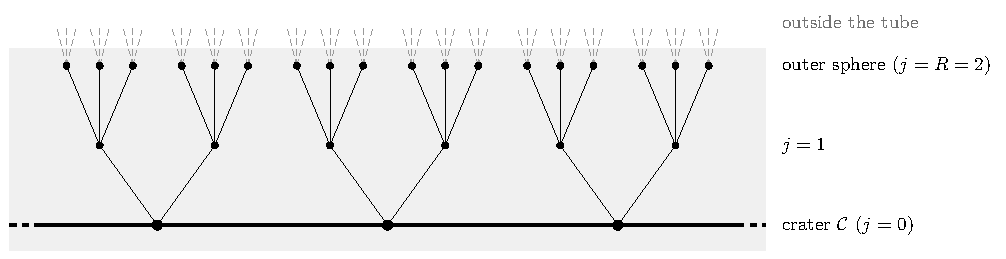
\includegraphics[width=0.85\linewidth]{tube}
\caption{The tube for a split prime, drawn with \(p=3\) and \(R=2\) for legibility. Every vertex has \(p+1\) neighbors. A crater vertex has two neighbors along the crater and \(p-1\) outward ones; a vertex at distance \(1\) has one inward and \(p\) outward neighbors, all of them siblings; on the outer sphere only the inward neighbor carries a sibling, and the dashed edges lead out of the tube, where no member lies.}
\label{fig:tube}
\end{figure}

\begin{lemma}[Tube lemma]\label{lem:tube}
Let \(X\) be a member.
\begin{enumerate}
\item[(a)] \(0\le j(X)\le R\), and \(P_X\cong\mathbb Z/p^{R+j}\times\mathbb Z/p^{R-j}\) with \(j=j(X)\).
\item[(b)] If \(j(X)<R\), then \(X[p]=p^{-1}\Lambda_X/\Lambda_X\cong\mathbb F_p^2\): the \(p+1\) lines of \(X[p]\) are the \(p+1\) neighbors of \(\Lambda_X\), and \(X\) has a sibling at each. Call a line \emph{inward} if its sibling is not farther from \(\mathcal C\), and \emph{outward} otherwise; write \(\mathrm{Out}(X)\) for the set of outward lines and \(\nu(X)\) for the number of inward ones. Off the crater there is exactly one inward line \(D_X\), and there are \(p\) outward ones. On a split crater the two inward lines are the \emph{crater lines} \(T_{\mathfrak p}=\mathfrak p_{\mathcal O}^{-1}I_X/I_X\) and \(T_{\bar{\mathfrak p}}\), along which the crater runs; on an inert crater there is none. So \(|\mathrm{Out}(X)|=p\), \(p-1\) or \(p+1\).
\item[(c)] If \(j(X)=R\), that is, if \(X\) lies on the \emph{outer sphere}, then \(P_X\) is cyclic of order \(p^{2R}\), so \(X[p]\) is a single line \(D_X\), and it is inward.
\item[(d)] For an outward line \(T\), the image of \(X[p]\) in \(G_{X_T}\) is the inward line \(D_{X_T}\).
\end{enumerate}
\end{lemma}

\begin{proof}
All members share \(\varepsilon_0\), the root greater than \(1\) of \(x^2-(\operatorname{tr}\gamma_0)x+1\), and \(\varepsilon_0\) maps each member's lattice onto itself. So the question is which vertices \(\varepsilon_0\) stabilizes. Write \(w:=\varepsilon_0^{-1}-1=p^Ru\) with \(u\in\mathfrak o\smallsetminus p\mathfrak o\).

We first show that \(\mathbb Z_p[\varepsilon_0]=\mathfrak o_R\). Since \(\varepsilon_0\) has norm \(1\), \((1+p^Ru)(1+p^R\bar u)=1\), so \(u+\bar u=-p^Ru\bar u\equiv0\pmod p\). Moreover \(u\) is a unit of \(\mathfrak o\): if \(p\) is inert, because \(\mathfrak o\) is local with maximal ideal \(p\mathfrak o\) and \(u\notin p\mathfrak o\); if \(p\) splits, because conjugation swaps the two coordinates of \(\mathfrak o\cong\mathbb Z_p\times\mathbb Z_p\) and \(u+\bar u\equiv0\) makes both coordinates of \(u\) nonzero modulo \(p\). If \(u\) were congruent to some \(a\in\mathbb Z_p\) modulo \(p\mathfrak o\), then so would be \(\bar u\), and \(2a\equiv0\). As \(p\) is odd, this would give \(u\in p\mathfrak o\), which is excluded. The same holds for \(u^{-1}\). So \(1,u\) is a basis of \(\mathfrak o\), and \(\mathbb Z_p[\varepsilon_0]=\mathbb Z_p+\mathbb Z_pp^Ru=\mathfrak o_R\). Hence
\[\varepsilon_0\Lambda=\Lambda\iff\varepsilon_0\in\mathrm{End}\,\Lambda=\mathfrak o_j\iff\mathfrak o_R\subseteq\mathfrak o_j\iff j\le R .\]
Every member therefore lies in the tube \(\{j\le R\}\) around the crater. The labels of \(X\) are \(w^{-1}I_X/I_X\), whose \(p\)-part is \(w^{-1}\Lambda_X/\Lambda_X\cong\mathfrak o_j/w\mathfrak o_j\). This group has order \(|\mathrm{Nm}\,w|_p^{-1}=p^{2R}\), as \(u\) is a unit, and exponent \(p^{R+j}\), as \(u^{-1}\notin\mathbb Z_p+p\mathfrak o\). This proves (a).

For \(j<R\) we have \(p^{R-1}u\in\mathfrak o_j\), so \(p^{-1}\Lambda\subseteq w^{-1}\Lambda\) and all of \(p^{-1}\Lambda/\Lambda\) consists of labels. This proves (b). At \(j=R\) the group is cyclic and its single line is fixed by \(\varepsilon_0\). So its sibling is \(\varepsilon_0\)-stable, hence not outside the tube, and it is the inward neighbor. This proves (c). For (d), if \(T\) is outward, the sibling lattice \(\Lambda':=\Lambda+\widetilde T\) lies in \(p^{-1}\Lambda\), and the image of \(X[p]\) is \(p^{-1}\Lambda/\Lambda'\). Adding it to \(\Lambda'\) gives \(p^{-1}\Lambda\), the vertex of \(X\), which is one step nearer to the crater than \(\Lambda'\).
\end{proof}

Norm one is essential here: in \(\mathbb Q(\sqrt5)\), the element \(12+121\varphi=1+11(1+11\varphi)\) is \(\equiv1\pmod{11}\) but generates only \(\mathfrak o_2\).

As an example, let \(\gamma=\bigl(\begin{smallmatrix}2&1\\1&1\end{smallmatrix}\bigr)\), so that \(K=\mathbb Q(\sqrt5)\), \(\tau^*=\varphi=(1+\sqrt5)/2\), \(\varepsilon=\varphi^2\), \(I_\gamma=O_K\), \(N_\gamma=1\) and \(f=1\). At \(p=11=(3+2\varphi)(5-2\varphi)\) one has \(k_0=5\), \(\gamma_0=\bigl(\begin{smallmatrix}89&55\\55&34\end{smallmatrix}\bigr)\), \(\varepsilon_0=\varphi^{10}=55\varphi+34\) and \(\varepsilon_0-1=11(5\varphi+3)\) with \(5\varphi+3\) a unit, so \(R=1\). The labels of \(\gamma_0\) are \(\tfrac1{11}O_K/O_K\cong\mathbb F_{11}^2\), on the crater. Its \(12\) lines give \(2\) siblings along the crater and \(10\) on the outer sphere, for instance \(\bigl(\begin{smallmatrix}89&605\\5&34\end{smallmatrix}\bigr)\) with lattice \(\mathbb Z\varphi+\tfrac1{11}\mathbb Z\). The labels of that sibling form a cyclic group of order \(121\), generated by \((5\varphi-8)/121\), and its single line \(\{\tfrac a{11}\varphi\}\) leads back to the crater vertex of \(\gamma_0\).

\subsubsection*{Two code bounds from the Fourier identity}
Identity (vi) says that the normalized Fourier transform \(\mathcal F\) on \(G_X\) reproduces \(E_X\) up to the root of unity \(\lambda q(y)\) and the reflection \(y\mapsto-y\); applying \(\mathcal F\) once more, with \(\mathcal F^2f(y)=f(-y)\) and \(q\) even, gives \(\mathcal F(qE_X)=\lambda^{-1}E_X\). Because \(\mathcal F\) divides by \(|G_X|^{1/2}\), these identities impose divisibility on weighted sums of the values. Write \(G_X=P_X\oplus Q_X\) with \(Q_X\) of order prime to \(p\). The pairing and \(q\) split along this decomposition. Indeed, for \(x\in P_X\) and \(y\in Q_X\), \(b(x,y)\) has order dividing \(|P_X|\) and \(|Q_X|\), so \(b(x,y)=1\). The identity \(q(x+y)=q(x)q(y)b(x,y)\), which follows from~\cite[(3)]{RW}, then gives \(q(x+y)=q(x)q(y)\). As \(b\) is nondegenerate on \(G_X\)~\cite[\S4.3]{RW}, so is its restriction to \(P_X\). Let \(\mathcal F_P\) and \(\mathcal F_Q\) be the transforms on \(P_X\) and \(Q_X\), normalized by \(|P_X|^{-1/2}\) and \(|Q_X|^{-1/2}\), let \(q_P\) and \(q_Q\) be the restrictions of \(q\), and put, with \(P:=P_X\),
\[\mathfrak L(P):=\{f:P\to\mathcal O_v\ :\ \mathcal F_Pf,\ \mathcal F_P(q_Pf)\ \text{integral}\},\]
with integrality in \(\mathcal O_v\). We call such integral lattices of functions \emph{codes}, and bounds on the reductions of their elements \emph{code bounds}.

\begin{lemma}[Column lemma]\label{lem:column}
Let \(X\) be a member and \(\beta\in K_{\mathrm{fam}}^\times\). If \(\beta E_X\) is integral, then for every \(c\in Q_X\) the \emph{column} \(f_c(x):=\beta E_X(x+c)\), \(x\in P_X\), lies in \(\mathfrak L(P_X)\).
\end{lemma}

\begin{proof}
By the two identities above, \(\beta E_X\), \(\mathcal F(\beta E_X)\) and \(\mathcal F(q\beta E_X)\) are all integral. Since the pairing and \(q\) split, \(\mathcal F=\mathcal F_P\otimes\mathcal F_Q\), and for a function \(F\) on \(G_X\) we have \((\mathcal F_P\otimes1)F=(1\otimes\mathcal F_Q^{-1})\mathcal FF\). The kernel of \(\mathcal F_Q^{-1}\) is \(|Q_X|^{-1/2}\) times roots of unity, a \(v\)-unit as \(p\nmid|Q_X|\). We apply this to \(F=\beta E_X\) and \(F=q\beta E_X\), whose transforms are integral. Since \(q\beta E_X(x+c)=q_{Q}(c)\,q_P(x)\beta E_X(x+c)\) with \(q_Q(c)\) a root of unity, every column \(f_c\) lies in \(\mathfrak L(P_X)\).
\end{proof}

Lemma~\ref{lem:column} is the only use of~\cite[(6)]{RW} in Sections~\ref{sec:local}, \ref{sec:root} and~\ref{sec:rec}. On the outer sphere \(P_X\) is cyclic of order \(p^{2R}\). For a generator \(g\) put \(\zeta:=q(g)\). Then \(q(xg)=q(g)^{x^2}=\zeta^{x^2}\) and \(b(xg,yg)=q((x+y)g)/(q(xg)q(yg))=\zeta^{2xy}\). As \(b\) is nondegenerate on \(P_X\) and \(p\) is odd, \(\zeta^2\) has order \(p^{2R}\); and \(\zeta^{p^{4R}}=q(p^{2R}g)=q(0)=1\), so \(\zeta\) has odd order and is a primitive \(p^{2R}\)-th root of unity.

\begin{proposition}[Cyclic code theorem]\label{prop:code}
Let \(P=\mathbb Z/p^{n}\) with \(n=2R\), let \(\zeta\) be a primitive \(p^n\)-th root of unity, \(q(x)=\zeta^{x^2}\), \((\mathcal Ff)(y)=p^{-n/2}\sum_x\zeta^{2xy}f(x)\) and \(m:=(p^n+2)/3\). For every valuation ring \(\mathcal O\) of a field of characteristic \(0\) with \(\zeta\in\mathcal O\) and residue characteristic \(p\ge5\), the reduction of \(\mathfrak L_{\mathcal O}(P)\) lies in the span of the binomial functions \(\binom{x}{i}\) with \(i\le m\).
\end{proposition}

We use only the consequence for the top base-\(p\) digit of \(i\), stated after the proof.

\begin{proof}
Write \(\mathcal Rf(x):=f(-x)\), \(\mathcal Tf(x):=f(x-1)\), \(\Delta:=\mathcal T-1\) and \(\mathcal U:=q^{-1}\mathcal F^{-1}\), where \(q\) also denotes multiplication by \(q\). For a field \(k\) of characteristic \(p\) and \(j\le p^n\) let \(\mathcal D_j\subseteq k^P\) be the span of the functions \(x\mapsto\binom xi\), \(0\le i<j\), read on the representatives \(0\le x<p^n\). Steps~1--3 take place over a field of characteristic \(0\), Steps~4--6 over one discrete valuation ring, and Step~7 passes to an arbitrary valuation ring.

\emph{Step 1: Gauss sums and \(\mathcal U^3=I\).} For \(m\ge0\) and \(p\nmid a\) put \(G_m(a):=\sum_{x\bmod p^m}\zeta_m^{ax^2}\), with \(\zeta_m:=\zeta^{p^{n-m}}\) a primitive \(p^m\)-th root of unity. For \(m\ge2\) write \(x=x_0+p^{m-1}x_1\) with \(0\le x_0<p^{m-1}\) and \(x_1\bmod p\). As \(2m-2\ge m\), we have \(ax^2\equiv ax_0^2+2ax_0x_1p^{m-1}\pmod{p^m}\), and the sum over \(x_1\) is \(p\) if \(p\mid x_0\) and \(0\) otherwise. Writing \(x_0=py\) gives \(G_m(a)=pG_{m-2}(a)\), and \(G_0(a)=1\). As \(n\) is even,
\[G(a):=\sum_{x\in P}\zeta^{ax^2}=p^R\qquad(p\nmid a).\]
The kernel of \(\mathcal F\) is \(p^{-R}\zeta^{2xy}\). Since \(\sum_y\zeta^{2y(x+z)}=p^n\) if \(x=-z\) and \(0\) otherwise, \(\mathcal F^2=\mathcal R\), so \(\mathcal F^{-1}=\mathcal R\mathcal F\) has kernel \(p^{-R}\zeta^{-2xy}\). The kernel of \(\mathcal F^{-1}q^{-1}\mathcal F^{-1}\) is therefore
\[p^{-2R}\sum_z\zeta^{-2yz-z^2-2zx}=p^{-2R}\zeta^{(x+y)^2}G(-1)=p^{-R}\zeta^{(x+y)^2},\]
which is the kernel of \(q\mathcal Fq\). Hence \(\mathcal F^{-1}q^{-1}\mathcal F^{-1}=q\mathcal Fq\), and \(\mathcal U^3=q^{-1}(\mathcal F^{-1}q^{-1}\mathcal F^{-1})q^{-1}\mathcal F^{-1}=I\). The reflection \(\mathcal R\) commutes with \(q\), which is even, and with \(\mathcal F\), whose kernel is invariant under \((x,y)\mapsto(-x,-y)\). Hence it commutes with \(\mathcal U\).

\emph{Step 2: The lattice.} For a valuation ring \(\mathcal O\) as in the statement write \(\mathfrak L_{\mathcal O}:=\mathfrak L_{\mathcal O}(P)\). As \(\mathcal U^{-1}=\mathcal U^2=\mathcal Fq\) and \(\mathcal U=q^{-1}\mathcal R\mathcal F\), and as \(q^{\pm1}\) and \(\mathcal R\) preserve \(\mathcal O^P\), a function \(f\) lies in \(\mathfrak L_{\mathcal O}\) if and only if \(f\), \(\mathcal Uf\) and \(\mathcal U^2f\) lie in \(\mathcal O^P\). Since \(\mathcal U^3=I\), this condition holds for \(\mathcal Uf\) whenever it holds for \(f\). So \(\mathfrak L_{\mathcal O}\) is stable under \(\mathcal U\), and also under \(\mathcal R\), which commutes with \(\mathcal U\) and preserves \(\mathcal O^P\).

\emph{Step 3: Multiplicities.} Over a field of characteristic \(0\) containing \(\zeta\) and a primitive cube root of unity, the kernels of Step~1 give the kernels
\begin{align*}
\mathcal U&:\ p^{-R}\zeta^{-y^2-2xy},&\mathcal U^2=\mathcal Fq&:\ p^{-R}\zeta^{2xy+x^2},\\
\mathcal U\mathcal R=q^{-1}\mathcal F&:\ p^{-R}\zeta^{-y^2+2xy},&\mathcal U^2\mathcal R=\mathcal F^{-1}q&:\ p^{-R}\zeta^{x^2-2xy}.
\end{align*}
Their traces are \(p^{-R}G(c)\) with \(c=-3,3,1,-1\), all equal to \(1\) by Step~1, since \(p\ne3\). The trace of \(\mathcal R\) is the number of \(x\) with \(x=-x\), which is \(1\). For a character \(\vartheta=(\xi,\sigma)\) of \(\mathbb Z/3\times\mathbb Z/2\), with \(\xi^3=1\) and \(\sigma=\pm1\), let \(V_\vartheta\) be the space of \(f\) with \(\mathcal Uf=\xi f\) and \(\mathcal Rf=\sigma f\). The representation \((i,j)\mapsto\mathcal U^i\mathcal R^j\) of \(\mathbb Z/3\times\mathbb Z/2\) shows that
\[n_\vartheta:=\dim V_\vartheta=\frac16\sum_{i,j}\overline{\vartheta(i,j)}\,\tr(\mathcal U^i\mathcal R^j)=\frac{p^n-1}6+\delta_{\vartheta,1},\]
because the five nonidentity traces equal \(1\), the identity has trace \(p^n\), and \(p^n\equiv1\pmod6\).

\emph{Step 4: Decomposition over a discrete valuation ring.} Let \(A_1\) be the localization of \(\mathbb Z[\zeta,\zeta_3]\) at a maximal ideal containing \(p\), with fraction field \(K_1\) and residue field \(k_1\). It is a discrete valuation ring in which \(6\) is a unit, as \(p\ge5\). The idempotents
\[e_\vartheta:=\frac16\sum_{i,j}\overline{\vartheta(i,j)}\,\mathcal U^i\mathcal R^j\]
have coefficients in \(A_1\), so they preserve \(\mathfrak L_{A_1}\) by Step~2. They sum to \(I\), and \(e_\vartheta\) projects \(K_1^P\) onto \(V_\vartheta\). Put \(\mathfrak L_\vartheta:=V_\vartheta\cap A_1^P\). If \(f\in\mathfrak L_\vartheta\), then \(\mathcal U^{\pm1}f=\xi^{\pm1}f\) is integral, so \(\mathfrak L_\vartheta\subseteq\mathfrak L_{A_1}\). Hence \(\mathfrak L_{A_1}=\bigoplus_\vartheta\mathfrak L_\vartheta\). Each \(\mathfrak L_\vartheta\) is a free \(A_1\)-module of rank at most \(n_\vartheta\), so its reduction \(U_\vartheta\subseteq k_1^P\) has dimension at most \(n_\vartheta\), and the reduction of \(\mathfrak L_{A_1}\) is \(\sum_\vartheta U_\vartheta\).

\emph{Step 5: A reduced Laplacian.} Let \(\mathcal M_bf(x):=\zeta^{2bx}f(x)\). From the kernel of \(\mathcal F\) one reads off \(\mathcal F\mathcal T=\mathcal M_1\mathcal F\) and \(\mathcal F\mathcal M_b=\mathcal T^{-b}\mathcal F\); hence \(\mathcal F^{-1}\mathcal T=\mathcal M_{-1}\mathcal F^{-1}\) and \(\mathcal T\mathcal F^{-1}=\mathcal F^{-1}\mathcal M_1\). Moreover \(q(x)/q(x-1)=\zeta^{2x-1}\) gives \(q\mathcal T=\zeta^{-1}\mathcal M_1\mathcal Tq\). Therefore
\[\mathcal U\mathcal T\mathcal U^{-1}=q^{-1}\mathcal F^{-1}\mathcal T\mathcal Fq=\mathcal M_{-1},\]
\[\mathcal U^{-1}\mathcal T\mathcal U=\mathcal Fq\mathcal Tq^{-1}\mathcal F^{-1}=\zeta^{-1}\mathcal F\mathcal M_1\mathcal F^{-1}\mathcal M_1=\zeta^{-1}\mathcal T^{-1}\mathcal M_1,\]
and, taking inverses, \(\mathcal U\mathcal T^{-1}\mathcal U^{-1}=\mathcal M_1\) and \(\mathcal U^{-1}\mathcal T^{-1}\mathcal U=\zeta\mathcal M_{-1}\mathcal T\). So
\[Z:=\sum_{i=0}^{2}\mathcal U^i(\mathcal T+\mathcal T^{-1})\mathcal U^{-i}=\mathcal T+\mathcal T^{-1}+\mathcal M_{-1}+\mathcal M_1+\zeta^{-1}\mathcal T^{-1}\mathcal M_1+\zeta\mathcal M_{-1}\mathcal T .\]
Conjugation by \(\mathcal U\) permutes the three summands in the definition, as \(\mathcal U^3=I\), so \(Z\) commutes with \(\mathcal U\). It commutes with \(\mathcal R\), as \(\mathcal R\mathcal T\mathcal R=\mathcal T^{-1}\). By the second expression \(Z\) has entries in \(\mathbb Z[\zeta]\). Hence \(Z\) preserves \(A_1^P\) and every \(V_\vartheta\), hence every \(\mathfrak L_\vartheta\), and its reduction \(\bar Z\) preserves every \(U_\vartheta\). As \(\zeta\equiv1\) modulo the maximal ideal, \(\mathcal M_b\) reduces to the identity and
\[\bar Z=2(\mathcal T+1+\mathcal T^{-1}).\]
Since \(2\) is invertible in \(k_1\), the operator \(Y:=\tfrac12\bar Z-3=\mathcal T-2+\mathcal T^{-1}=\mathcal T^{-1}\Delta^2\) preserves every \(U_\vartheta\).

\emph{Step 6: Degrees.} On \(k_1^P\) we have \(\Delta^{p^n}=\mathcal T^{p^n}-1=0\), so \(Y\) is nilpotent, and \(Y^{n_\vartheta}=0\) on \(U_\vartheta\), whose dimension is at most \(n_\vartheta\). As \(\mathcal T\) is invertible and commutes with \(\Delta\), \(\Delta^{2n_\vartheta}=\mathcal T^{n_\vartheta}Y^{n_\vartheta}\) kills \(U_\vartheta\).

To turn this into a degree bound, we claim that \(\ker\Delta^j=\mathcal D_j\) for \(j\le p^n\). By Lucas's theorem, for \(i<p^n\) the residue of \(\binom xi\) depends only on \(x\bmod p^n\), so the identity \(\binom{x+1}i-\binom xi=\binom x{i-1}\) holds on \(P\). The functions \(\binom xi\), \(0\le i<p^n\), form a basis of \(k^P\), since the matrix \(\bigl(\binom xi\bigr)_{0\le x,i<p^n}\) is unitriangular. So the forward difference \(\delta:=\mathcal T^{-1}-1\) sends \(\binom xi\) to \(\binom x{i-1}\) for \(i\ge1\) and \(\binom x0\) to \(0\), whence \(\ker\delta^j=\mathcal D_j\). Finally \(\Delta=-\mathcal T\delta\) gives \(\ker\Delta^j=\ker\delta^j\). Therefore \(U_\vartheta\subseteq\mathcal D_{2n_\vartheta}\). The largest value of \(2n_\vartheta\) is \((p^n+5)/3=m+1\), so the reduction of \(\mathfrak L_{A_1}\) lies in \(\mathcal D_{m+1}\), the span of the \(\binom xi\) with \(i\le m\).

\emph{Step 7: Arbitrary valuation rings.} It remains to pass from \(A_1\) to the valuation ring \(\mathcal O\) of the statement. First, \(A_0:=\mathcal O\cap\mathbb Q(\zeta)\) is a valuation ring of \(\mathbb Q(\zeta)\) whose maximal ideal contains \(p\). It contains \(\mathbb Z[\zeta]\), the ring of integers, so it is the localization of \(\mathbb Z[\zeta]\) at the prime \((1-\zeta)\), the only prime above \(p\). In particular \(A_0\) is a discrete valuation ring with fraction field \(K_0=A_0[1/p]=\mathbb Q(\zeta)\), and the maximal ideal of \(\mathcal O\) meets \(A_0\) in that of \(A_0\). Choose \(A_1\) in Step~4 above \(A_0\), that is, localize at a maximal ideal containing \(1-\zeta\). The residue fields then satisfy \(k_0\subseteq k_1\) and \(k_0\subseteq k_{\mathcal O}\), compatibly with reduction.

We next bound the reduction of \(\mathfrak L_{A_0}\). Since \(\mathfrak L_{A_0}\subseteq\mathfrak L_{A_1}\), Step~6 shows that this reduction lies in \(k_0^P\cap(k_1\otimes\mathcal D_{m+1})=k_0\otimes\mathcal D_{m+1}\). The equality holds because \(\mathcal D_{m+1}=\ker\Delta^{m+1}\) is cut out by equations with coefficients in \(\mathbb F_p\).

Finally we extend scalars from \(A_0\) to \(\mathcal O\). The module \(\mathfrak L_{A_0}\) is the kernel of
\[A_0^P\to(K_0/A_0)^{2P},\qquad f\mapsto\bigl(\mathcal Ff,\ \mathcal F(qf)\bigr)\bmod A_0 .\]
As \(\mathcal O\) is torsion-free over the discrete valuation ring \(A_0\), it is flat. Tensoring with \(\mathcal O\) therefore gives the exact sequence
\[0\to\mathcal O\otimes\mathfrak L_{A_0}\to\mathcal O^P\to(\mathcal O[1/p]/\mathcal O)^{2P},\]
whose second map is again \(f\mapsto(\mathcal Ff,\mathcal F(qf))\bmod\mathcal O\). Hence \(\mathfrak L_{\mathcal O}\) is the \(\mathcal O\)-span of an \(A_0\)-basis \((b_i)\) of the free module \(\mathfrak L_{A_0}\), and the reduction of \(\sum c_ib_i\) is \(\sum\bar c_i\,\overline{b_i}\in k_{\mathcal O}\otimes\mathcal D_{m+1}\). This argument uses neither the rank of the valuation nor completeness, and the residue field of \(\mathcal O\) may be transcendental over \(\mathbb F_p\).
\end{proof}

We use Proposition~\ref{prop:code} in the following form. Along a coset of the subgroup of order \(p\), the position moves only in its top base-\(p\) digit, and every \(i\le m\) has top base-\(p\) digit at most \(\lfloor m/p^{n-1}\rfloor\), which equals \(\lfloor p/3\rfloor\) (write \(p=3J+r\) with \(r\in\{1,2\}\)). So by Lucas's theorem the residue is a polynomial in the coordinate \(u\in\mathbb F_p\) of the coset of degree at most
\[J:=\lfloor p/3\rfloor;\qquad\text{note that }p-2J\ge3\text{ for }p\ge5 .\]

\begin{lemma}[Envelope]\label{lem:envelope}
Let \(p\) be any prime, \(2\) and \(3\) included, let \(P=(\mathbb Z/p^r)^2\), and let \(\mathcal O\) be a valuation ring containing a primitive \(p^r\)-th root of unity (so of characteristic \(0\)), with residue characteristic \(p\). If \(f:P\to\mathcal O\) has all character sums \(\sum_x\chi(x)f(x)\) in \(p^r\mathcal O\), then the residue of \(f\) on each coset of \(P[p]\) is a polynomial of total degree \(\le p-1\) in any affine coordinates on the coset.
\end{lemma}

The proof of Theorem~\ref{thm:D} uses Lemma~\ref{lem:envelope} at every prime, \(2\) and \(3\) included. For a nondegenerate pairing the hypothesis says that \(f\) and \(\mathcal Ff\) are integral; on the crater, where \(P_X\cong(\mathbb Z/p^R)^2\), the lemma applies to every column.

\begin{proof}
Let \(\zeta\in\mathcal O\) be a primitive \(p^r\)-th root of unity and \(\varpi:=\zeta-1\). In \(\mathbb Z[\zeta]\), for \(1\le j<p^r\) the element \(\zeta^j-1\) is a unit times \(\varpi^{p^{v_p(j)}}\), and \(p\) is a unit times \(\varpi^{\varphi(p^r)}\). For an element \(c\) of \(\mathbb Z[\zeta]\) of the form \(\text{unit}\cdot\varpi^e\) we write \(\mathrm{ord}(c):=e\).

The characters of \(P\) are \(x\mapsto\zeta^{-(sx_1+tx_2)}\), \((s,t)\in P\), so the hypothesis says that \(\mathcal Ff(s,t):=p^{-r}\sum_x\zeta^{-(sx_1+tx_2)}f(x)\) is integral for all \((s,t)\). Translating \(f\) multiplies every character sum by a root of unity, so it suffices to treat the coset \(P[p]\).

For \(0\le a<p^r\) put
\[D_a:=\prod_{i<a}(\zeta^a-\zeta^i),\qquad g_a(x):=\frac1{D_a}\prod_{i<a}(\zeta^x-\zeta^i)\qquad(x\in\mathbb Z/p^r).\]
On the representatives \(0\le x<p^r\), \(g_a(x)=0\) for \(x<a\) and \(g_a(a)=1\), and for \(x\ge a\)
\[g_a(x)=\prod_{j=1}^{a}\frac{\zeta^{x-a+j}-1}{\zeta^j-1}=\begin{bmatrix}x\\ a\end{bmatrix}_\zeta\in\mathbb Z[\zeta],\]
the Gaussian binomial coefficient at \(\zeta\). So the matrix \((g_a(x))_{x,a}\) is unitriangular with entries in \(\mathbb Z[\zeta]\), and the functions \(g_a\otimes g_b:(x_1,x_2)\mapsto g_a(x_1)g_b(x_2)\) form a basis of \(\mathcal O^P\). Thus \(f=\sum c_{ab}\,g_a\otimes g_b\) is integral if and only if every \(c_{ab}\) is integral.

To express the integrality of \(\mathcal Ff\) in the same coordinates, write \(\prod_{i<a}(Z-\zeta^i)=\sum_{k=0}^aT_{ka}Z^k\), so that \(T_{ka}\in\mathbb Z[\zeta]\), \(T_{aa}=1\) and \(T_{ka}=0\) for \(k>a\). Then \(g_a(x)=D_a^{-1}\sum_kT_{ka}\zeta^{kx}\), and for \(0\le s<p^r\) orthogonality gives \(\sum_x\zeta^{-sx}g_a(x)=p^rT_{sa}/D_a\). Hence
\[\mathcal Ff(s,t)=\sum_{a,b}T_{sa}T_{tb}\,\frac{p^r\,c_{ab}}{D_aD_b}.\]
The matrix \((T_{sa})\) is unitriangular over \(\mathbb Z[\zeta]\), so \(\mathcal Ff\) is integral if and only if every \(p^rc_{ab}/(D_aD_b)\) is integral. Now \(\zeta^a-\zeta^i=\zeta^i(\zeta^{a-i}-1)\), so \(\mathrm{ord}(D_a)=\mathrm{wt}(a):=\sum_{j=1}^ap^{v_p(j)}\), while \(\mathrm{ord}(p^r)=r\varphi(p^r)\). Therefore \(f\) and \(\mathcal Ff\) are integral if and only if
\[c_{ab}\in\varpi^{e_{ab}}\mathcal O,\qquad e_{ab}:=\max\bigl(0,\ \mathrm{wt}(a)+\mathrm{wt}(b)-r\varphi(p^r)\bigr).\]

We now restrict to \(P[p]=\{(p^{r-1}s,p^{r-1}t):0\le s,t<p\}\). Modulo \(\varpi\) we have \(\zeta\equiv1\), so \(g_a(x)\equiv\binom xa\); for \(x<a\) both sides vanish. By Lucas's theorem \(\binom{p^{r-1}s}{a}\equiv0\pmod p\) unless \(a=p^{r-1}A\) with \(0\le A<p\), in which case it is \(\equiv\binom sA\). For such \(a\), counting the \(j\le p^{r-1}A\) divisible by \(p^k\) for \(1\le k\le r-1\) gives
\[\mathrm{wt}(p^{r-1}A)=Ap^{r-1}+\sum_{k=1}^{r-1}(p^k-p^{k-1})\,Ap^{r-1-k}=Ap^{r-2}\bigl(r(p-1)+1\bigr).\]
If \(A+B\ge p\), then
\[\mathrm{wt}(p^{r-1}A)+\mathrm{wt}(p^{r-1}B)-r\varphi(p^r)\ge p^{r-1}\bigl(r(p-1)+1\bigr)-rp^{r-1}(p-1)=p^{r-1}>0,\]
so the corresponding coefficient has residue \(0\). Hence the residue of \(f\) on \(P[p]\) is
\[\bar f(p^{r-1}s,p^{r-1}t)=\sum_{A+B\le p-1}\bar c_{p^{r-1}A,\,p^{r-1}B}\binom sA\binom tB.\]
Here \(\binom sA\) is a polynomial of degree \(A\) in \(s\) over \(\mathbb F_p\), as \(A<p\). So the residue is a polynomial of total degree at most \(p-1\). Such a polynomial has partial degrees less than \(p\), so it is the unique reduced representative of its function on \(\mathbb F_p^2\), and an \(\mathbb F_p\)-linear change of coordinates does not raise its total degree. No step divides by \(2\) or \(3\).
\end{proof}

\subsubsection*{The defect identity}
A pole cannot be followed directly from a member to an outward sibling. By (ii) the sibling's value has the sum of the valuations along a line, and values of positive valuation on that line can cancel the pole. The proof therefore follows a different quantity. For a line \(T\) put \(L_T(y):=\prod_{h\in T}E_X(y+h)\), put \(\Pi_X(y):=\prod_{h\in X[p]}E_X(y+h)\), and recall that \(\nu(X)\) is the number of inward lines. The \emph{defect} is
\[\Theta_X(y):=E_X(y)^{-p^2}\,\Pi_X(y)^{1-\nu(X)}\prod_{T\ \text{inward}}L_T(y)^p,\]
that is, \(\bigl(L_{D_X}(y)/E_X(y)^p\bigr)^p\) off the crater, \((L_{T_{\mathfrak p}}L_{T_{\bar{\mathfrak p}}})^p/(E_X^{p^2}\Pi_X)\) on a split crater, and \(\Pi_X/E_X^{p^2}\) on an inert crater. Numerator and denominator contain the same number of values, so \(\Theta_X(y)=1\) when \(E_X\) is constant on \(y+X[p]\). Off the crater, \(\Theta_X(y)\) measures how far the values along the inward line through \(y\) are from being equal.

\begin{lemma}[Defect identity]\label{lem:defect}
If \(j(X)<R\), then
\[\Theta_X(y)^p=\prod_{T\ \text{outward}}\Theta_{X_T}(\pi_Ty),\]
an identity in \(K_{\mathrm{fam}}^\times\).
\end{lemma}

\begin{proof}
We use two exact identities. The first is the \emph{vertex identity}: the \(p+1\) lines through \(y\) cover \(y\) exactly \(p+1\) times and every other point of \(y+X[p]\) once, so \(\prod_TL_T(y)=E_X(y)^p\,\Pi_X(y)\). The second is the \emph{edge identity}. For an outward line \(T\), the \(p\) translates of \(T\) inside \(y+X[p]\) map onto the inward line of \(X_T\) through \(\pi_Ty\) (Lemma~\ref{lem:tube}(d)), and (ii), with the same \(\kappa_T\) on every translate, gives
\[\Pi_X(y)=\kappa_T^{\,p}L_{D_{X_T}}(\pi_Ty),\qquad L_T(y)=\kappa_TE_{X_T}(\pi_Ty).\]
By the vertex identity and the count of outward lines, \(\Theta_X(y)=\prod_{T\ \text{outward}}\Pi_X(y)/L_T(y)^p\). By the edge identity the \(p\)-th power of each factor is \(\Theta_{X_T}(\pi_Ty)\), the roots of unity cancelling.
\end{proof}

The exponent \(1-\nu(X)\) is what makes \(\Pi_X\) appear once for every outward line. Nothing is reduced and nothing is assumed about the values; the identity needs only that \(\kappa_T\) does not depend on the translate, which is part of (ii).

The defect is needed because the sharp bound \(J=\lfloor p/3\rfloor\) requires \(P_X\) to be cyclic, which happens only on the outer sphere. Elsewhere only Lemma~\ref{lem:envelope} is available, and its bound \(p-1\) along a line gives \(p-2(p-1)<0\), which yields nothing. This is why a pole must first be turned into a defect and carried outward.

\subsubsection*{Proof of the local theorem}
Put \(\theta_X(y):=v(\Theta_X(y))\), a real number since no value is \(0\) by (i).

\begin{lemma}[Transport]\label{lem:transport}
If \(j(X)<R\), then \(p\,\theta_X(y)=\sum_{T\ \text{outward}}\theta_{X_T}(\pi_Ty)\). Consequently there are a member \(Y\) on the outer sphere and a label \(y'\) of \(Y\) with \(\theta_Y(y')\ge\theta_X(y)\) if \(j(X)\ge1\), and \(\theta_Y(y')\ge\tfrac{p}{|\mathrm{Out}(X)|}\theta_X(y)\) if \(j(X)=0\).
\end{lemma}

\begin{proof}
The formula follows by taking valuations in Lemma~\ref{lem:defect}. Off the crater there are \(p\) outward lines, so \(\theta_X(y)\) is the mean of the outward values, and some outward sibling has \(\theta\) at least as large. On the crater the first step multiplies the bound by \(p/(p-1)\) (split) or \(p/(p+1)\) (inert). Every outward neighbor is again a member, so iterating reaches the outer sphere.
\end{proof}

\begin{lemma}[Outer-boundary inequality]\label{lem:outer}
If \(j(X)=R\) and \(a:=a(X)>0\), then \((p-2J)\,a\le a(X_D)\), where \(X_D\) is the sibling of \(X\) along \(D_X\).
\end{lemma}

\begin{proof}
Choose \(y_0\) with \(v(E_X(y_0))=-a\) and put \(\beta:=E_X(y_0)^{-1}\), so that \(\beta E_X\) is integral. Along \(y_0+D\) the residue of \(\beta E_X\) is a polynomial of degree \(\le J\) (Proposition~\ref{prop:code} and Lucas's theorem) taking the value \(1\) at \(y_0\). So it vanishes at most \(J\) times, and \(v(E_X)=-a\) at no fewer than \(p-J\) points of \(y_0+D\). At the remaining points \(v(E_X)\le a\) by the reflection bound. By (ii) the product along \(y_0+D\) is a root of unity times a value of the inward sibling \(X_D\), so \(-a(X_D)\le-(p-J)a+Ja\).
\end{proof}

\begin{proof}[Proof of \textup{(U0)}]
Let \(A:=\max_Xa(X)\), a maximum over finitely many values, and suppose that \(A>0\), attained at \((X_0,y_0)\). By the reflection bound, \(|v(E_X(y))|\le A\) everywhere. Below the outer sphere also \(|v(\Pi_X(y))|\le A\): by the edge identity and (ii) at \(X_T\), \(\Pi_X(y)\) is a root of unity times a single value of the member whose lattice is \(p^{-1}I_X\), a homothetic copy of \(I_X\).

The member \(X_0\) is not on the outer sphere, since there Lemma~\ref{lem:outer} would give a pole of size at least \((p-2J)A\ge3A\). Its defect at \(y_0\) is large. Off the crater, \(\theta_{X_0}(y_0)=p\,v(E_{X_D})-p^2v(E_{X_0}(y_0))\ge p(p-1)A\); on an inert crater, \(\theta_{X_0}(y_0)\ge(p^2-1)A\); on a split crater, \(\theta_{X_0}(y_0)\ge(p^2-2p-1)A\). By Lemma~\ref{lem:transport} there are \(Y\) on the outer sphere and \(y'\) with \(\theta_Y(y')\ge cA\), where \(c=p(p-1)\) when starting off the crater or on an inert crater, and \(c=p(p^2-2p-1)/(p-1)\) when starting on a split crater.

This produces a pole on the outer sphere. There \(\theta_Y(y')=p\,v(L_{D_Y}(y'))-p^2v(E_Y(y'))\le pA-p^2v(E_Y(y'))\), so \(a(Y)\ge\rho A\) with \(\rho=c/p^2-1/p\), that is, \(\rho=(p-2)/p\) or \(\rho=(p-3)/(p-1)\). One step inward, Lemma~\ref{lem:outer} at \(Y\) gives
\[a(Y_D)\ge(p-2J)\rho A\ge3\rho A>A,\]
since \(3(p-2)/p>1\) and \(3(p-3)/(p-1)>1\) for \(p\ge5\). This contradicts the choice of \(A\). So \(A=0\), and with the reflection bound \(v(E_X(y))=0\) for every value.
\end{proof}

For \(p=7\), starting off the crater, the numbers are \(\theta\ge42A\), then \(a(Y)\ge\tfrac57A\), then \(a(Y_D)\ge\tfrac{15}7A\). Apart from Lemma~\ref{lem:outer}, the argument uses only that \(v\) turns products into sums and that a maximum is at least a mean. The hypothesis \(p\ge5\) is used twice: \(6\) must be a unit in Proposition~\ref{prop:code}, and \(p-2J\ge3\) (with \(3\rho>1\)) closes the contradiction; at \(p=3\), \(p-2J=1\).

\begin{proof}[Proof of \textup{(U1)} and \textup{(U2)}]
By (U0) every defect is a unit. Suppose that some \(\Theta_Y\not\equiv1\), and take such a \(Y\) with \(j(Y)\) maximal.

On the outer sphere this is impossible. The residues of \(E_Y\) along the translates of \(D_Y\) through \(y\) and through \(-y\) are polynomials of degree \(\le J\), and reflection makes their product (one of them read backwards) a nonzero constant. Indeed \(E_Y(y+h)E_Y(-y-h)=q(y+h)^{-1}\), and for \(h\in P_Y\) the ratio \(q(y+h)/q(y)\) is a root of unity of \(p\)-power order, hence \(\equiv1\); where the origin occurs, use \(E_Y(0)^2=\varepsilon_0\equiv1\). We use the \emph{pairing lemma}: two polynomials over a field whose degrees add up to less than \(p\), and whose product takes the same nonzero value at all \(p\) points of \(\mathbb F_p\), are constant. As \(2J<p\), the residue of \(E_Y\) is constant along \(D_Y\), and \(\Theta_Y\equiv1\).

Below the outer sphere the outward siblings satisfy \(\Theta\equiv1\) by maximality, so Lemma~\ref{lem:defect} gives \(\Theta_Y(z)^p\equiv1\), hence \(\Theta_Y(z)\equiv1\), since \(x\mapsto x^p\) is injective on a field of characteristic \(p\). This proves (U1).

Off the crater, (U1) says that \(L_{D_X}(y)\equiv E_X(y)^p\). The left side is the same at every point of \(y+D_X\), and \(x\mapsto x^p\) is injective, so the residues of the values are constant along each translate of the inward line. On an inert crater the same argument gives constancy on each translate of \(X[p]\).

On a split crater write the points of \(y+X[p]\) as \(y+s+t\) with \(s\in T_{\mathfrak p}\) and \(t\in T_{\bar{\mathfrak p}}\). As \(L_T\) is \(T\)-invariant, (U1) gives \((\mathrm{red}\,E_X)^{p^2}(y+s+t)=\alpha(s)\beta(t)\) with \(\alpha\) and \(\beta\) nowhere zero. Lemma~\ref{lem:envelope} bounds the total degree of \(\mathrm{red}\,E_X\) by \(p-1\). Raising to the power \(p\) does not raise it: as a function on \(\mathbb F_p^2\), the \(p\)-th power of a polynomial is the polynomial with the \(p\)-th powers of its coefficients. So \(\alpha(s)\beta(t)\), as a reduced polynomial, has total degree \(\deg\alpha+\deg\beta\le p-1\), and likewise for the factors \(\alpha',\beta'\) at \(-y\). Reflection makes \(\alpha(s)\beta(t)\alpha'(-s)\beta'(-t)\) a nonzero constant, so \(\alpha(s)\alpha'(-s)\) and \(\beta(t)\beta'(-t)\) are each constant. By the pairing lemma a nonconstant pair would have degree sum at least \(p\), and two such pairs would exceed \(2(p-1)\). So \(\alpha\) or \(\beta\) is constant, which is (U2).
\end{proof}

Nothing local decides which of the two lines occurs. Every function on \(P_X\) that depends only on the coordinate along one crater line satisfies all three integrality conditions, so the dichotomy is the most the column lattice can give. The choice is made globally, in Section~\ref{sec:rec}.

\begin{proposition}[Algebraicity]\label{prop:alg}
Every value of~\cite{RW} is algebraic.
\end{proposition}

\begin{proof}
Fix a split prime \(p\ge5\) with \(p\nmid N_\gamma f\). Suppose that a value \(\xi\) were transcendental. Let \(L_0\) be a number field containing \(K\) and the roots of unity and square roots of the setting, and let \(F\) be the field generated over \(L_0\) by \(\xi\) and the values of the members; these are finitely many, by (vii), which does not use algebraicity. Extend \(\xi\) to a transcendence basis of \(F\) over \(L_0\). The weighted Gauss valuation over a prime of \(L_0\) above \(p\), normalized by \(v(p)=1\) and with weight \(v(\xi)<0\), is a discrete valuation of the rational function field, and it extends to a discrete valuation \(v\) of the finite extension \(F\). It satisfies the hypotheses of the setting, since no integrality of the values was assumed. Then (U0) would make \(\xi^{k_0}\) a unit, by (iii), a contradiction.
\end{proof}

This gives an independent proof of~\cite[Thm.~1]{RW}.

\subsection{Exact root extraction and the Frobenius congruence}\label{sec:root}

Theorem~\ref{thm:local} concerns the values of \(\gamma_0=\gamma^{k_0}\). The lines \(T_{\mathfrak p},T_{\bar{\mathfrak p}}\) consist of labels of \(\gamma_0\), not of \(\gamma\) (as \(p\nmid N_\gamma\)), and on the labels of \(\gamma\) the values of \(\gamma_0\) are \(k_0\)-th powers, by (iii). A congruence between \(k_0\)-th powers determines its base modulo \(\mathfrak P\mid p\) only up to a \(k_0\)-th root of unity, and this ambiguity does occur, since \(k_0\mid p-1\). So we take the root before reducing, among positive reals, where \(k_0\)-th roots are unique. The identities below are exact equalities of positive reals, and only the last step of Lemma~\ref{lem:root} reduces.

\begin{lemma}[Lattice distribution and positive orbit products]\label{lem:dist}
\begin{enumerate}
\item[(a)] Suppose that \(\varepsilon'\) is a totally positive unit with \(\varepsilon'_r>1\). Let \(I\subseteq I'\) be lattices with \(\varepsilon'I=I\) and \(I'/I\subseteq t_{\varepsilon'}^{-1}I/I\). Then for every \(z\in t_{\varepsilon'}^{-1}I\) with \(z\notin I'\),
\[\prod_{y\in I'/I}W(I,\varepsilon',z+y)=W(I',\varepsilon',z).\]
\item[(b)] Let \(I\subseteq I'\) be lattices of finite index and \(u\) a unit with \(uI=I\), \(uI'=I'\), \(|u_r|>1\) and \(u_u>0\). Put \(m(u):=1\) if \(u_r>0\) and \(m(u):=2\) otherwise, and let \(\mathcal W(I,u,x):=W(I,u^{m(u)},x)^{1/m(u)}\) be the positive root. Let \(z\in K\) with \((u-1)z\in I\) and \(z\notin I'\). For each \(\langle u\rangle\)-orbit \(O\) on \(I'/I\) choose \(h_O\in O\) and put \(d_O:=|O|\). Then
\[\mathcal W(I',u,z)=\prod_O\mathcal W(I,u^{d_O},z+h_O),\]
an identity of positive reals, independent of the representatives \(h_O\).
\end{enumerate}
\end{lemma}

\begin{proof}[Proof of (a)]
Since \(\varepsilon'\) fixes \(t_{\varepsilon'}^{-1}I/I\) pointwise, every lattice between \(I\) and \(I'\) is \(\varepsilon'\)-stable. A composition series of \(I'/I\), with the product grouped by cosets, therefore reduces (a) to one step \(L\subset L'\) of prime index \(p\). Let \((v_1,v_2)\) be a fixed frame of \(L\) and \(\gamma\) the matrix of \(\varepsilon'\) in it, so that \(L=v_2I_\gamma\), and let \(T\subset G_\gamma\) be the line \(L'/L\) read in \(I_\gamma\). Taking absolute squares in the line product formula (ii), with \(|\kappa_T|=1\) and \(|E|^2=w\) by (iv), gives \(\prod_{h\in T}w_\gamma(x+h)=|E_{\gamma_T}(\pi_Tx)|^2\). The content of the lemma is that the right side is \(W(L',\varepsilon',z)\), with the same \(z\) and exponent \(+1\); this needs the sibling's frame. In~\cite[Prop.~9]{RW}, the sibling is \(\gamma_T=N_T\gamma N_T^{-1}\) with
\[N_T=\begin{pmatrix}1&f/y\\0&h/y\end{pmatrix},\qquad h,y\ge1,\ hy=p,\ f\in\mathbb Z,\]
and \(\pi_T\) sends the label \((\ell,j)\) to \((h\ell,\,yj-f\ell)\). Then \(N_T(\tau^*,1)^{\mathsf T}=(h/y)(\tau',1)^{\mathsf T}\) with \(\tau':=(y\tau^*+f)/h\), so \(\tau'\) is the attracting fixed point of \(\gamma_T\), and \(\gamma_T\) is the matrix of \(\varepsilon'\) on \(L_0':=\mathbb Zv_1'+\mathbb Zv_2'\), where \(v_1':=\tau'/y\) and \(v_2':=1/y\). This frame is fixed: \(v_2'\) is a positive rational, and \(\tau'_r-\tau'_u=(y/h)(\tau^*_r-\tau^*_u)>0\); both facts come from \(\det N_T>0\) and the lower row \((0,h/y)\) of \(N_T\). The label map is the identity on elements: if \((\varepsilon'^{-1}-1)x=\ell\tau^*+j\), the image label gives \(h\ell\tau'+(yj-f\ell)=y(\ell\tau^*+j)\), which is \(x\) read in the frame with second vector \(1/y\). Finally \(\tau^*=hv_1'-fv_2'\) and \(1=yv_2'\), so \(I_\gamma\subset L_0'\) with index \(p\), and \(\ker\pi_T=T\); hence \(L_0'=I_\gamma+\widetilde T\). So \(\prod_{h\in T}W(I_\gamma,\varepsilon',x+h)=W(I_\gamma+\widetilde T,\varepsilon',x)\), and multiplying by \(v_2\gg0\) gives the step.
\end{proof}

The orientation of the sibling frame matters. If its second vector were not totally positive, or if \(\theta_r<\theta_u\), the frame rules of Section~\ref{sec:sign} would replace the right side by \(W(L',\varepsilon',\pm z)^{\pm1}\); the upper triangular \(N_T\) with \(\det N_T>0\) excludes this. Part (a) uses only (ii), (iv) and (vii).

\begin{proof}[Proof of (b)]
Let \(n\) be divisible by \(m(u)\) and by the order of \(u\) on \(I'/I\). Then \(u^n\) is totally positive with \(u^n_r>1\), fixes \(I'/I\) pointwise and satisfies \((u^n-1)z\in I\). So (a) at \(\varepsilon'=u^n\) gives \(W(I',u^n,z)=\prod_{h\in I'/I}W(I,u^n,z+h)\); all these points lie off \(I\), as \(z\notin I'\). By (iii) the left side is \(\mathcal W(I',u,z)^n\). Homothety by \(u\) ((viii), with \(uI=I\) and \(u_u>0\)) makes \(W(I,u^n,z+\cdot)\) constant on \(\langle u\rangle\)-orbits, because \(u(z+h)\equiv z+uh\pmod I\). On an orbit \(O\), \(u^{d_O}\) fixes \(z+h_O\) modulo \(I\), so \(z+h_O\) is a label of the totally positive unit \(u^{d_Om(u^{d_O})}\), and \(d_Om(u^{d_O})\) divides \(n\): if \(m(u^{d_O})=2\), then \(u_r<0\) and \(d_O\) is odd, while \(2=m(u)\) and \(d_O\) both divide \(n\). By (iii), \(W(I,u^n,z+h_O)=\mathcal W(I,u^{d_O},z+h_O)^{n/d_O}\), and the \(d_O\) equal factors of \(O\) contribute \(\mathcal W(I,u^{d_O},z+h_O)^n\). Take positive \(n\)-th roots.
\end{proof}

When \(u\) is a power of the unit \(\varepsilon\) whose matrix is used, as in Lemma~\ref{lem:root}, homothety by \(u\) is the \(\varepsilon\)-invariance in (vii), and Theorem~\ref{thm:DC} is not used. Section~\ref{sec:partB} applies (b) to a unit of norm \(-1\).

\subsubsection*{Setting for root extraction}
Let \(\gamma\) be the matrix of \(\varepsilon\) in a fixed frame \((v_1,v_2)\) of \(I\), let \(\mathcal O:=\mathrm{End}(I)\), of conductor \(f\), and let \(p=\mathfrak p\bar{\mathfrak p}\) be a split prime with \(p\ge5\) and \(p\nmid N_\gamma f\). Let \(\mathfrak q\in\{\mathfrak p,\bar{\mathfrak p}\}\) and \(\mathfrak q_{\mathcal O}:=\mathfrak q\cap\mathcal O\), an invertible prime of degree one. Since \(\varepsilon\) has norm \(1\), \(\varepsilon\bmod\bar{\mathfrak p}\) is the conjugate of \((\varepsilon\bmod\mathfrak p)^{-1}\), so the order of \(\varepsilon\) in \((\mathcal O/\mathfrak q_{\mathcal O})^\times\cong\mathbb F_p^\times\) is the \(k_0\) of Section~\ref{sec:local}; in particular \(k_0\mid p-1\). As \(\varepsilon^{k_0}\equiv1\pmod{\mathfrak q_{\mathcal O}}\), the line
\[T:=\mathfrak q_{\mathcal O}^{-1}I_\gamma/I_\gamma\subset G_{\gamma_0}\]
is the crater line \(T_{\mathfrak q}\) of Theorem~\ref{thm:local}. It is a one-dimensional \(\mathcal O/\mathfrak q_{\mathcal O}\)-vector space on which \(\varepsilon\) acts as a scalar of order \(k_0\), so \(\varepsilon\) acts freely on \(T\smallsetminus0\) with \(\ell:=(p-1)/k_0\) orbits; let \(h_1,\dots,h_\ell\) represent them. Moreover \(k_0>1\), since \(p\nmid N_\gamma=-\mathrm{Nm}(\varepsilon-1)\), while \(\varepsilon\) fixes \(G_\gamma\) pointwise; hence \(T\cap G_\gamma=0\).

\begin{lemma}[Root extraction]\label{lem:root}
For \(x\in G_\gamma\smallsetminus0\) and \(z:=v_2x\),
\[W(\mathfrak q_{\mathcal O}^{-1}I,z)=W(I,z)\cdot\prod_{i=1}^{\ell}w_{\gamma_0}(x+h_i),\]
an identity of positive reals, independent of the representatives \(h_i\); no root of unity and no Gaussian factor appears. If, at a prime \(\mathfrak P\mid p\) of a field containing the values involved, these values are \(\mathfrak P\)-units and the residue of \(E_{\gamma_0}\) is constant on \(x+T\), then
\[W(\mathfrak q_{\mathcal O}^{-1}I,z)\equiv W(I,z)^p\pmod{\mathfrak P}.\]
\end{lemma}

\begin{proof}
By a totally positive homothety we may take \(I=I_\gamma\) and \(v_2=1\). The identity is Lemma~\ref{lem:dist}(b) with \(u=\varepsilon\) and \(I'=\mathfrak q_{\mathcal O}^{-1}I_\gamma\), so that \(I'/I=T\). Since \(T\cap G_\gamma=0\), we have \(z\notin I'\). The \(\langle\varepsilon\rangle\)-orbits on \(T\) are \(\{0\}\), contributing \(W(I,\varepsilon,z)=w_\gamma(x)=:w_x\), and the \(\ell\) orbits of the \(h_i\), of length \(k_0\), contributing \(W(I,\varepsilon^{k_0},z+h_i)=w_{\gamma_0}(x+h_i)\), as \(\gamma_0\) is the matrix of \(\varepsilon^{k_0}\) in the same frame.

For the congruence, \(w_{\gamma_0}(x+h)=q_{\gamma_0}(x+h)E_{\gamma_0}(x+h)^2\) and \(q_{\gamma_0}(x+h)=q_{\gamma_0}(x)\,q_{\gamma_0}(h)\,b(x,h)\), where the last two factors are roots of unity of \(p\)-power order (as \(ph=0\)), hence \(\equiv1\). With the constancy of the residue on \(x+T\) and (iii), \(w_{\gamma_0}(x+h_i)\equiv w_{\gamma_0}(x)=w_x^{k_0}\). So the right side is \(\equiv w_x^{1+k_0\ell}=w_x^{p}\).
\end{proof}

The exponent count \(1+k_0\ell=p\) is exact: it counts the source point \(x\) and \(\ell\) orbits of length \(k_0\). Before any root is taken, (ii) on the single coset \(x+T\) reads \((E_\gamma(x)\Pi_x)^{k_0}=\kappa\,E_{\gamma_{\mathfrak q}}(x')^{k_0}\), where \(\Pi_x:=\prod_iE_{\gamma_0}(x+h_i)\), \(\kappa\) is a root of unity, and \(\gamma_{\mathfrak q}\) is the matrix of \(\varepsilon\) on \(\mathfrak q_{\mathcal O}^{-1}I\); by (iii), \(\gamma_{\mathfrak q}^{k_0}\) is the sibling of \(\gamma_0\) along \(T\). Lemma~\ref{lem:root} takes the positive \(k_0\)-th root of its absolute value, so the value of \(\kappa\) never enters.

\begin{definition}[Good primes]\label{def:good}
Fix a lattice \(I\) and a unit \(\varepsilon\) as in a datum, with matrix \(\gamma\) in a fixed frame, and a finite Galois extension \(L/K\) containing the values of all admissible matrices of trace \(\operatorname{tr}\varepsilon\); these form a finite set by (vii), and they are algebraic by Proposition~\ref{prop:alg}. A rational prime \(p\) is \emph{good} for \((\varepsilon,L)\) if \(p\ge5\), \(p\) splits in \(K\), \(p\nmid N_\gamma f_0\) (so that \(p\nmid f\), as \(f\mid f_0\)), and \(p\) is unramified in \(L\).
\end{definition}

This notion depends on \(I\) only through \(\varepsilon\), and all but finitely many split primes are good. The root extraction, the Frobenius congruence and every Chebotarev step below need only such a cofinite set.

\begin{lemma}[Frobenius congruence]\label{lem:frob}
Let \(p=\mathfrak p\bar{\mathfrak p}\) be good for \((\varepsilon,L)\) and let \(\mathfrak P\mid\mathfrak p\) be a prime of \(L\). Then for every \(z\in t_\varepsilon^{-1}I\smallsetminus I\) the values involved are \(\mathfrak P\)-units, and
\[W(I,z)^p\equiv W(\mathfrak p_{\mathcal O}^{-1}I,z)\quad\text{or}\quad W(I,z)^p\equiv W(\bar{\mathfrak p}_{\mathcal O}^{-1}I,z)\pmod{\mathfrak P}.\]
\end{lemma}

\begin{proof}
Extend \(v_{\mathfrak P}\), normalized by \(v(p)=1\), to a valuation \(v\) of a field \(K_{\mathrm{fam}}\supseteq L\) as in the setting of Theorem~\ref{thm:local}, whose hypotheses hold (\(p\ge5\) split, \(p\nmid N_\gamma f\)). By (U0) every value of every member is a \(v\)-unit; in particular \(E_\gamma(x)\), whose \(k_0\)-th power is \(E_{\gamma_0}(x)\), is one. By (U2) at \(x=z/v_2\) there is \(\mathfrak q\in\{\mathfrak p,\bar{\mathfrak p}\}\) such that the residue of \(E_{\gamma_0}\) is invariant under \(T_{\mathfrak q}\), hence constant on \(x+T_{\mathfrak q}\). Lemma~\ref{lem:root} gives \(W(\mathfrak q_{\mathcal O}^{-1}I,z)\equiv W(I,z)^p\) modulo the maximal ideal of \(v\). Both sides lie in \(L\), so the congruence holds modulo \(\mathfrak P\).
\end{proof}

As \(\mathrm{Frob}_{\mathfrak P}\) acts on \(O_L/\mathfrak P\) as the \(p\)-th power map, Lemma~\ref{lem:frob} says that \(\mathrm{Frob}_{\mathfrak P}W(I,z)\) is congruent to one of two candidates. The statement is symmetric under \(\mathfrak p\leftrightarrow\bar{\mathfrak p}\), and the candidate can belong to \(\bar{\mathfrak p}\) although \(\mathfrak P\) lies above \(\mathfrak p\).

\subsection{The reciprocity law}\label{sec:rec}

We first set up the action of ideles on data. The lattice \(s_f^{-1}I\) of Section~\ref{sec:results} has the same multiplier ring as \(I\). Indeed, the multiplier ring of a lattice \(L\) is \(K\cap\prod_\ell\mathrm{End}(L_\ell)\), where \(L_\ell:=L\otimes\mathbb Z_\ell\). The completion of \(s_f^{-1}I\) at \(\ell\) is \(s_\ell^{-1}I_\ell\), and multiplication by the unit \(s_\ell^{-1}\) of the commutative ring \(K\otimes\mathbb Q_\ell\) does not change the multiplier ring. Moreover \((\varepsilon-1)s_f^{-1}z=s_f^{-1}(\varepsilon-1)z\) lies in \(s_f^{-1}\widehat I\), and \(s_f^{-1}z\notin s_f^{-1}\widehat I\). So \(s^{-1}d\) is again a datum, and \((st)^{-1}d=t^{-1}(s^{-1}d)\).

Fix \(\varepsilon\) and put \(\mathfrak M:=\mathfrak M_\varepsilon=f_0(\varepsilon-1)O_K\). Let \(U_{\mathfrak M}\) be the group of ideles \(s\) with \(s_{\mathfrak q}\in1+\mathfrak MO_{\mathfrak q}\) for \(\mathfrak q\mid\mathfrak M\) and \(s_{\mathfrak q}\in O_{\mathfrak q}^\times\) otherwise, with arbitrary infinite components; let \(U_{\mathfrak M}^+\) be its subgroup with \(s_r,s_u>0\), and \(U_{\mathfrak M,f}\) its finite part. Then
\[C_{\mathfrak M}=\mathbb A_K^\times/K^\times U_{\mathfrak M}^+\cong\mathbb A_{K,f}^\times/K^\times_{\gg0}U_{\mathfrak M,f},\]
and \(\mathrm{Art}\) identifies this group with \(\mathrm{Gal}(H_{\mathfrak M\infty_r\infty_u}/K)\). Let \(c_r,c_u\) be the classes of \((1;-1,1)\) and \((1;1,-1)\); then \(\mathrm{Art}(c_v)\) is the complex conjugation \(\iota_v\) restricted to \(H_{\mathfrak M\infty_r\infty_u}\). Let \(\Omega_\varepsilon\) be the set of data with unit \(\varepsilon\), modulo \(z\mapsto z+I\) and \((I,z)\mapsto(\beta I,\beta z)\) for \(\beta\gg0\). It is finite: finitely many orders contain \(\mathbb Z[\varepsilon]\), each has finitely many narrow classes of invertible \(\mathcal O\)-ideals, and each lattice has finitely many labels. The value \(W\) is a function on \(\Omega_\varepsilon\).

\begin{lemma}[Ray classes acting on data]\label{lem:rayclass}
The following hold for data of every order.
\begin{enumerate}
\item[(a)] \(\mathfrak M\) is \(\tau\)-stable, and \(\mathfrak Mz\subseteq I\) for every datum \((I,\varepsilon,z)\).
\item[(b)] \(d\mapsto s_f^{-1}d\) induces an action of \(C_{\mathfrak M}\) on \(\Omega_\varepsilon\). If \(s\) is the finite idele of an integral ideal \(\mathfrak a\) prime to \(\mathfrak M\), then \(s^{-1}(I,\varepsilon,z)=(\mathfrak a_{\mathcal O}^{-1}I,\varepsilon,z)\), where \(\mathfrak a_{\mathcal O}:=\mathfrak a\cap\mathcal O_I\).
\item[(c)] For \(a\in\mathbb Z\) prime to \(\mathfrak M\) and \(\pi\gg0\) with \(\pi\equiv a\ (\mathrm{mod}\ \mathfrak M)\), \([(\pi)]\cdot(I,z)=(I,az)\). For \(\beta\equiv1\ (\mathrm{mod}\ \mathfrak M)\) with \(\beta_r<0<\beta_u\), \(c_r\cdot(I,z)=(\beta^{-1}I,z)\). Moreover \(c_rc_u\cdot(I,z)=(I,-z)\).
\item[(d)] The involution \(c\mapsto\bar c\) of \(C_{\mathfrak M}\) induced by \(\tau\) satisfies \(\bar c_r=c_u\) and \(\overline{[\mathfrak p]}=[\bar{\mathfrak p}]\).
\end{enumerate}
\end{lemma}

\begin{proof}
(a) We have \(\tau(\varepsilon-1)=-\varepsilon^{-1}(\varepsilon-1)\), and \(f_0O_K\subseteq\mathbb Z[\varepsilon]\subseteq\mathcal O_I\) gives \(\mathfrak Mz\subseteq I\).

(b) \(K^\times_{\gg0}\) acts trivially, since the action commutes with homotheties. An element \(u\in U_{\mathfrak M,f}\) has \(u_\ell^{\pm1}\in\mathcal O_{I,\ell}\) at every \(\ell\) (at \(\ell\mid f_0\) because \(1+\mathfrak M_\ell\subseteq\mathbb Z[\varepsilon]_\ell\)), so \(u^{-1}\widehat I=\widehat I\) and \((u^{-1}-1)z\in\mathfrak Mz\subseteq I\). For \(\mathfrak a\) prime to \(\mathfrak M\) the idele is \(1\) wherever \(z_\ell\ne0\) or \(\ell\) divides the conductor of \(I\), which gives \((\mathfrak a_{\mathcal O}^{-1}I,z)\) \cite[Prop.~7.20]{Cox}.

(c) \([(\pi)]\cdot(I,z)=(\pi^{-1}I,z)\sim(I,\pi z)=(I,az)\), as \((\pi-a)z\in\mathfrak Mz\subseteq I\). The principal idele \(\beta\) is the product of the idele of \((\beta)\), an element of \(U_{\mathfrak M}^+\), and \((1;\beta_r,\beta_u)\); hence \([(\beta)]=c_r\). For \(\beta\equiv1\) totally negative, \(\pi:=-\beta\) is the case \(a=-1\).

(d) By (a), \(\tau\) preserves \(U_{\mathfrak M}\) and \(K^\times\), so it induces an involution of \(C_{\mathfrak M}\). It exchanges the two real places, so it maps \((1;-1,1)\) to \((1;1,-1)\), and it maps the idele of \(\mathfrak p\) to that of \(\tau\mathfrak p=\bar{\mathfrak p}\).
\end{proof}

\begin{lemma}[The ordering bit]\label{lem:orderbit}
Let \(\mathbb A_K^\times\) act on \((\text{data})\times\{\pm1\}\) by \(s\star(d,\epsilon):=(s^{-1}d,\,\epsilon\operatorname{sgn}s_u)\), and put \(V(d,\epsilon):=W(d)^\epsilon\), so that the right side of~\eqref{eq:star} is \(V(s\star(d,1))\). Then \(V(s\star x)=V(x)\) for \(s\in U_{\mathfrak M}^+\), for \(s=(1;s_r,s_u)\) with \(s_u>0\), and for \(s=\alpha\in K^\times\) with \(\mathrm{Nm}\,\alpha>0\). Moreover \(V(\alpha\star x)=V(x)\) for all \(\alpha\in K^\times\) if and only if the homothety law (viii) holds. Hence, given (viii), \(V(s\star x)\) depends only on the class of \(s\) in \(C_{\mathfrak M}\).
\end{lemma}

\begin{proof}
\(U^+_{\mathfrak M}\) acts trivially by Lemma~\ref{lem:rayclass}(b), and archimedean ideles do not move \(d\). With \(\beta=\alpha^{-1}\), \(V(\alpha\star(d,\epsilon))=W(\beta I,\beta z)^{\epsilon\operatorname{sgn}\alpha_u}\), which equals \(W(d)^\epsilon\) exactly when (viii) holds for \(\beta\). For \(\mathrm{Nm}\,\beta>0\) this is frame independence, with reflection if \(\beta\ll0\).
\end{proof}

The Chebotarev argument below determines the Galois action on each value only up to a choice between two candidates. The following lemma removes the ambiguity.

\begin{lemma}[Selector]\label{lem:selector}
Let a finite abelian group \(\widetilde C\), with an involutive automorphism \(c\mapsto\bar c\) and elements \(c_r,c_u\) with \(\bar c_r=c_u\), act on a finite set \(\Omega\). Let \(F\subset\mathbb R\) be a field, \(W:\Omega\to F_{>0}\), and \(\varphi:\widetilde C\to\mathrm{Aut}(F)\) a homomorphism with
\begin{enumerate}
\item[(Sel1)] \(\varphi(c)W(\omega)\in\{W(c\omega),W(\bar c\omega)\}\) for all \(c,\omega\);
\item[(Sel2)] \(\varphi(c_r)=1\);
\item[(Sel3)] \(W(c_r\omega)=W(\omega)\) and \(W(c_u\omega)=W(\omega)^{-1}\) for all \(\omega\).
\end{enumerate}
Then \(\varphi(c)W(\omega)=W(c\omega)\) for all \(c,\omega\).
\end{lemma}

\begin{proof}
Put \(x:=\varphi(c)W(\omega)\). By (Sel2), \(x=\varphi(cc_r)W(\omega)\), and (Sel1) at \(cc_r\), with \(\overline{cc_r}=\bar cc_u\) and (Sel3), gives \(x\in\{W(c\omega),W(\bar c\omega)^{-1}\}\). By (Sel1) at \(c\), \(x\in\{W(c\omega),W(\bar c\omega)\}\). If \(x\ne W(c\omega)\), then \(x=W(\bar c\omega)=W(\bar c\omega)^{-1}\) is a positive real equal to its inverse, so \(x=1\) and \(W(\omega)=\varphi(c)^{-1}(1)=1\). The same dichotomy for \(c^{-1}\) at \(c\omega\) gives \(\varphi(c)^{-1}W(c\omega)\in\{W(\omega),1\}=\{1\}\), so \(W(c\omega)=1=x\), a contradiction.
\end{proof}

Both (Sel2) and (Sel3) are needed. The analogous values at the repelling fixed point satisfy every hypothesis except (Sel3). Let \(m\) be the least common multiple of \(24\) and the orders of the values of \(q\); when \(K\cap\mathbb Q(\mu_m)=\mathbb Q\), the inverted conjugates \(1/\sigma W\), for \(\sigma|_K=\tau\) with \(\sigma(\zeta)=\zeta^{-1}\) on \(\mu_m\), satisfy every hypothesis except (Sel2).

\begin{lthm}{RL}[Artin law on \(\Omega_\varepsilon\)]\label{thm:RL}
Let \(F_\varepsilon:=K(W(\omega):\omega\in\Omega_\varepsilon)\).
\begin{enumerate}
\item[(RL1)] \(F_\varepsilon\subseteq H_{\mathfrak M\infty_u}\); in particular \(F_\varepsilon/K\) is abelian and \(\iota_r\) is trivial on \(F_\varepsilon\).
\item[(RL2)] \(\mathrm{Art}(c)W(\omega)=W(c\omega)\) for every \(\tau\)-fixed class \(c\). In particular \(\mathrm{Art}([(\pi)])W(I,z)=W(I,az)\) for \(\pi\gg0\), \(\pi\equiv a\ (\mathrm{mod}\ \mathfrak M)\) with \(a\in\mathbb Z\), and \(\mathrm{Art}(c_u)W(\omega)=W(\omega)^{-1}\).
\item[(RL3)] \(\mathrm{Art}(c)W(\omega)=W(c\omega)\) for every \(c\in C_{\mathfrak M}\) and every \(\omega\).
\end{enumerate}
\end{lthm}

\begin{proof}
For \(\omega=(I,z)\) the matrix \(\gamma\) of \(\varepsilon\) has \(\mathrm{Nm}(\varepsilon-1)=-N_\gamma\), so \(\mathrm{Nm}\,\mathfrak M=f_0^2N_\gamma\) and every good prime is prime to \(\mathfrak M\). Let \(L/K\) be a finite Galois extension containing \(H_{\mathfrak M\infty_r\infty_u}\) and every value of trace \(\operatorname{tr}\varepsilon\). The same good primes then work for every \(\omega\in\Omega_\varepsilon\).

\emph{Step 1: Chebotarev on a product of differences.} Let \(g\in\mathrm{Gal}(L/K)\) and \(c(g)\in C_{\mathfrak M}\) with \(\mathrm{Art}(c(g))=g|_{H_{\mathfrak M\infty_r\infty_u}}\). By Chebotarev's theorem \cite{Ch} there are infinitely many good degree-one primes \(\mathfrak p\) with a prime \(\mathfrak P\mid\mathfrak p\) of \(L\) such that \(\mathrm{Frob}_{\mathfrak P}=g\); for these, \([\mathfrak p]=c(g)\) and \([\bar{\mathfrak p}]=\overline{c(g)}\). At each such \(\mathfrak P\) we have \(gW(\omega)\equiv W(\omega)^p\), and Lemma~\ref{lem:frob}, with Lemma~\ref{lem:rayclass}(b), gives \(W(\omega)^p\equiv W(c(g)\omega)\) or \(W(\omega)^p\equiv W(\overline{c(g)}\omega)\). So the fixed algebraic number \(\bigl(gW(\omega)-W(c(g)\omega)\bigr)\bigl(gW(\omega)-W(\overline{c(g)}\omega)\bigr)\) lies in infinitely many primes, and is therefore \(0\):
\begin{equation}\tag{Cand}\label{eq:Cand}
g\,W(\omega)\in\bigl\{W(c(g)\,\omega),\ W(\overline{c(g)}\,\omega)\bigr\}\qquad(\omega\in\Omega_\varepsilon).
\end{equation}
No separation of distinct values is needed.

\emph{Step 2: Containment.} If \(g\) is trivial on \(H_{\mathfrak M\infty_r\infty_u}\), then \(c(g)=1\) and \(g\) fixes every \(W(\omega)\). So \(F_\varepsilon\subseteq H_{\mathfrak M\infty_r\infty_u}\).

\emph{Step 3: Reality at \(r\).} Each \(W(\omega)\) is a positive real and \(\Kab\subset\mathbb C\) lies above \(r\), so \(\mathrm{Art}(c_r)\), which is complex conjugation, fixes \(F_\varepsilon\). Hence \(F_\varepsilon\subseteq H_{\mathfrak M\infty_u}\), which is (RL1).

\emph{Step 4: \(\tau\)-fixed classes.} If \(\bar c=c\), the two candidates in~\eqref{eq:Cand} coincide, so \(\mathrm{Art}(c)W(\omega)=W(c\omega)\). Rational classes are \(\tau\)-fixed and act by \((I,z)\mapsto(I,az)\). The class \(c_rc_u\) is \(\tau\)-fixed and acts by \(z\mapsto-z\); by reflection (v) it therefore acts by inversion. With Step~3, \(\mathrm{Art}(c_u)=\mathrm{Art}(c_rc_u)\mathrm{Art}(c_r)^{-1}\) inverts every \(W(\omega)\). This is (RL2).

\emph{Step 5: Selection.} Put \(\varphi:=\mathrm{Art}(\cdot)|_{F_\varepsilon}\). As \(\mathrm{Gal}(L/K)\to C_{\mathfrak M}\) is onto, \eqref{eq:Cand} is (Sel1) for \(\Omega=\Omega_\varepsilon\), \(\widetilde C=C_{\mathfrak M}\) and the involution of Lemma~\ref{lem:rayclass}(d); Step~3 is (Sel2). For (Sel3), choose \(\beta\equiv1\ (\mathrm{mod}\ \mathfrak M)\) with \(\beta_r<0<\beta_u\); it exists, since \(1+\mathfrak M\) is a translate of a full lattice in \(\mathbb R^2\). Then \(c_r\cdot(I,z)=(\beta^{-1}I,z)\), and the homothety law (viii) for \(\beta\), which is the single use of Theorem~\ref{thm:DC}, gives \(W(\beta^{-1}I,z)=W(I,\beta z)=W(I,z)\), as \((\beta-1)z\in\mathfrak Mz\subseteq I\). Since \(c_u=c_rc_u\cdot c_r\), also \(W(c_u\omega)=W(c_r\omega)^{-1}=W(\omega)^{-1}\). Lemma~\ref{lem:selector} now gives (RL3).
\end{proof}

No hypothesis \(c_r\ne1\) is needed: if \(c_r=1\) then \(c_u=1\), and (RL2) forces \(W\equiv1\). The \(\tau\)-fixed classes form in general a proper subgroup of \(C_{\mathfrak M}\), so Step~5 is needed for the full law.

\begin{proof}[Proof of Theorem~\ref{thm:A}]
Algebraicity is Proposition~\ref{prop:alg}. Let \(d\) be a datum with unit \(\varepsilon\), \(\omega\) its class in \(\Omega_\varepsilon\), and \(s\in\mathbb A_K^\times\). By (RL1), \(W(d)\in H_{\mathfrak M\infty_u}\subseteq\Kab\).

\emph{Step 1.} Choose \(\alpha\in K^\times\) with \(\operatorname{sgn}\alpha_r=\operatorname{sgn}s_r\) and \(\operatorname{sgn}\alpha_u=\operatorname{sgn}s_u\) (one of \(\pm1,\pm\sqrt{d_K}\), with \(\sqrt{d_K}>0\) at \(r\)), and put \(s':=\alpha^{-1}s\). Then \(s'_r,s'_u>0\) and \(\mathrm{Art}_K(s)=\mathrm{Art}_K(s')\).

\emph{Step 2.} Since \((1;s'_r,s'_u)\in U^+_{\mathfrak M}\), the class \(c\) of \(s'\) in \(C_{\mathfrak M}\) is the class of its finite part \(s'_f\), and \(c\,\omega\) is the class of \((s'_f)^{-1}d\).

\emph{Step 3.} By (RL3), \(\mathrm{Art}_K(s')W(d)=W(c\omega)=W((s'_f)^{-1}d)\).

\emph{Step 4.} By Lemma~\ref{lem:orderbit}, that is, by (viii) for \(\alpha\),
\[W(s^{-1}d)^{\operatorname{sgn}s_u}=V(\alpha\star(s'\star(d,1)))=V(s'\star(d,1))=W((s'_f)^{-1}d).\]
Steps~3 and~4 give~\eqref{eq:star}.
\end{proof}

\subsubsection*{Rational and Galois forms}
Since \(W(d)\in\Kab\), the Galois form of Theorem~\ref{thm:A} is~\eqref{eq:star} itself.

Consider first rational ideles \(s\in\mathbb A_{\mathbb Q}^\times\subset\mathbb A_K^\times\). Then \(s_r=s_u\), so Step~1 of the proof of Theorem~\ref{thm:A} takes \(\alpha=\pm1\), Step~4 needs only the positive-norm case of Lemma~\ref{lem:orderbit}, and \(c\) is \(\tau\)-fixed, so Step~3 needs only (RL2). Thus the restriction of~\eqref{eq:star} to rational ideles uses neither Theorem~\ref{thm:DC} nor Lemma~\ref{lem:selector}. The transfer \(\mathrm{Ver}\) corresponds to the inclusion \(\mathbb A_{\mathbb Q}^\times\subset\mathbb A_K^\times\). For \(a\in\widehat{\mathbb Z}^\times\) we have \(a^{-1}z=a'z\) with \(a'\equiv a^{-1}\) an integer, and \(\chi_{\mathrm{cyc}}(\mathrm{Art}_{\mathbb Q}(a))=a^{-1}\); the real idele \(-1\) gives \(W(I,z)^{-1}=W(I,-z)\). Hence
\[\mathrm{Ver}(g)\,W(I,\varepsilon,z)=W(I,\varepsilon,\chi_{\mathrm{cyc}}(g)\,z)\qquad(g\in\mathrm{Gal}(\mathbb Q^{\mathrm{ab}}/\mathbb Q)).\]

Now let \(\sigma\in\mathrm{Gal}(\overline{\mathbb Q}/\mathbb Q)\) be arbitrary. If \(\sigma|_K=\mathrm{id}\), then \(\sigma F_\varepsilon=F_\varepsilon\subset\mathbb R\) by (RL1), and~\eqref{eq:Cand} makes \(\sigma W(\omega)\) a positive real. If \(\sigma|_K=\tau\), then \(\sigma^{-1}\iota\sigma\), with \(\iota\) complex conjugation, is the complex conjugation of the embedding \(\sigma\), which lies above \(u\). On \(F_\varepsilon\) it is \(\mathrm{Art}(c_u)\), so \(\iota\sigma W=\sigma(W^{-1})\) by (RL2), that is, \(|\sigma W|=1\). Hence
\[\overline{\sigma W(d)}=\sigma W(d)^{\chi_K(\sigma)}.\]
Only Steps~1--4 of the proof of Theorem~\ref{thm:RL} enter here, so Theorem~\ref{thm:DC} and Lemma~\ref{lem:selector} are not used. Section~\ref{sec:sic} uses this form.

\begin{remark}[What reciprocity cannot give]\label{rem:recnogo}
Let \(\mathfrak m\) be proper with \(c_u\ne1\) in \(\mathcal G_{\mathfrak m}\), let \(H:=H_{\mathfrak m\infty_u}\), and let \(y\in H^\times\) be totally positive. Then
\[Y(c):=\mathrm{Art}(c)\bigl(y/\mathrm{Art}(c_u)y\bigr)\qquad(c\in C_{\mathfrak m})\]
satisfies every clause that~\eqref{eq:star} imposes on a family indexed by \(C_{\mathfrak m}\). Yet \(y=1\) gives \(Y\equiv1\); and \(y=\pi^2\) with \((\pi)=\mathfrak Q^{h(H)}\), \(\mathfrak Q\) above a prime split completely in \(H\), gives \(v_{\mathfrak Q}(Y(1))=2h(H)\ne0\). So a family compatible with~\eqref{eq:star} need not generate anything beyond \(K\), nor consist of units. Generation needs an input about the numbers themselves, namely~\eqref{eq:N}; the unit property needs local ideles that change the lattice, as in the proof of Theorem~\ref{thm:D}.
\end{remark}

\subsection{Units at every finite prime}\label{sec:units}

For maximal-order data Theorem~\ref{thm:D} covers every finite prime, including \(2\), \(3\), ramified primes and primes dividing \(\varepsilon-1\). The proof has two parts. The \emph{anchors} make a value a unit at \(\mathfrak q\) whenever \(\mathfrak q\) divides the annihilator of its label, using~\eqref{eq:star} for ideles at \(\mathfrak q\). \emph{Propagation} carries this to all other labels, using (vi) at the prime in question.

Throughout this subsection lattices are invertible \(O_K\)-ideals. Fix a totally positive \(\varepsilon\in O_K^\times\) with \(\varepsilon_r>1\), and let \(\mathcal M_\varepsilon\) be the set of admissible \(\gamma\) with \(\operatorname{tr}\gamma=\operatorname{tr}\varepsilon\) and \(\mathrm{End}\,I_\gamma=O_K\), that is, the matrices of \(\varepsilon\) in fixed frames of invertible ideals. Their values form a finite set of algebraic numbers, by (vii) and Proposition~\ref{prop:alg}. Let \(F\) be a number field containing these values, the values of the finitely many intermediate orders used below, \(\mu_{24}\), \(\mu_{N}\) (where \(N=N_\varepsilon\)) and the square roots \(\sqrt{|P|}\), \(\sqrt{|Q|}\) below. Fix a rational prime \(p\), a prime \(\mathfrak Q\mid p\) of \(F\) with valuation \(v\), and put \(\mathfrak q:=\mathfrak Q\cap O_K\). Write \(G_\gamma=P\oplus Q\) for the decomposition into \(p\)-primary and prime-to-\(p\) parts. A label \(x\in G_\gamma=t_\varepsilon^{-1}I_\gamma/I_\gamma\) has a component \(x_{\mathfrak q'}\in K_{\mathfrak q'}/I_{\mathfrak q'}\) at each prime \(\mathfrak q'\), nonzero if and only if \(\mathfrak q'\mid\mathrm{Ann}(x)\). In product identities only, we put \(W(I,0):=\varepsilon\); this is consistent with (ii) on the origin coset, which gives \(\prod_{0\ne h\in T}W(I,h)=1\).

\begin{proposition}[Idelic anchors]\label{prop:anchors}
Let \(\gamma\in\mathcal M_\varepsilon\) and \(x\in G_\gamma\smallsetminus0\) with \(\mathfrak q\mid\mathrm{Ann}(x)\). Then \(W(I_\gamma,\varepsilon,x)\) and \(E_\gamma(x)\) are \(\mathfrak Q\)-units.
\end{proposition}

\begin{proof}
Write \(I=I_\gamma\) and \(W(I,x)=W(I,\varepsilon,x)\).

\emph{Step 1: Local units.} A finite idele supported at \(\mathfrak q\) has its Artin image in the decomposition group of \(\mathfrak Q\), which preserves \(v\), and has exponent \(+1\) in~\eqref{eq:star}. For \(a\in O_{\mathfrak q}^\times\) the idele \(a\) preserves \(I\) and replaces \(x_{\mathfrak q}\) by \(a^{-1}x_{\mathfrak q}\). So \(v(W(I,x))\) is constant on \(O_{\mathfrak q}^\times\)-orbits. Since \(I_{\mathfrak q}\) is free over \(O_{\mathfrak q}\), these orbits are the sets of labels with given other components and given \(\mathfrak q\)-annihilator exponent.

\emph{Step 2: Uniformizer.} Let \(s\) be the idele of a uniformizer at \(\mathfrak q\), so that \(s^{-1}I=J:=\mathfrak q^{-1}I\). If \(x_{\mathfrak q}=0\), then \(s^{-1}x\) and \(x\) define the same class in \(K/J\): at \(\mathfrak q\) both lie in \(J_{\mathfrak q}\), and \(s=1\) elsewhere. Hence, for such a nonzero label,
\begin{equation}\tag{L}\label{eq:L}
v(W(J,x))=v\bigl(\mathrm{Art}(s)W(I,x)\bigr)=v(W(I,x)).
\end{equation}

\emph{Step 3: Distribution.} If \(\mathfrak q\mid\mathrm{Ann}(x)\), then \(T:=J/I\subset G_\gamma\) has order \(\mathrm N\mathfrak q\), and Lemma~\ref{lem:dist}(a) for \(I\subset J\), extended to the origin coset by the convention above, gives
\begin{equation}\tag{D}\label{eq:D}
\prod_{h\in T}W(I,x+h)=W(J,x).
\end{equation}
For \(\mathrm N\mathfrak q=p^2\) this is two line products, through an intermediate lattice whose order may be non-maximal.

\emph{Step 4: Induction on \(r:=v_{\mathfrak q}(\mathrm{Ann}\,x)\ge1\).} If \(r=1\), the coset \(x+T\) contains exactly one label \(x_0\) with \((x_0)_{\mathfrak q}=0\), and the other \(\mathrm N\mathfrak q-1\) labels form a single \(O_{\mathfrak q}^\times\)-orbit, of common valuation \(a=v(W(I,x))\). Taking valuations in~\eqref{eq:D} and using~\eqref{eq:L} for \(x_0\equiv x\pmod J\),
\[v(W(I,x_0))+(\mathrm N\mathfrak q-1)\,a=v(W(J,x_0))=v(W(I,x_0)),\]
so \(a=0\); if \(x_0=0\), both outer terms are \(v(\varepsilon)=0\). If \(r\ge2\), all \(\mathrm N\mathfrak q\) labels \(x+h\) have \(\mathfrak q\)-exponent \(r\) and the same other components, so they form one orbit, of common valuation \(a\). In \(J\) the label \(x\) has \(\mathfrak q\)-exponent \(r-1\ge1\), so the induction hypothesis and~\eqref{eq:D} give \(\mathrm N\mathfrak q\cdot a=v(W(J,x))=0\).

Finally \(E_\gamma(x)^2=W/q(x)\), and \(q(x)\) is a root of unity.
\end{proof}

The argument is the same for dyadic, ramified and inert \(\mathfrak q\). It needs local ideles that change the lattice, through~\eqref{eq:L}: the families \(Y\) of Remark~\ref{rem:recnogo} obey the reciprocity law at a single modulus and are not units.

\begin{proof}[Proof of Theorem~\ref{thm:D}]
Fix \(p\), \(\mathfrak Q\) and \(\mathfrak q\) as above. By reflection (v) and \(E(0)^2=\varepsilon\), it suffices to show that every value is \(\mathfrak Q\)-integral.

\emph{Step 1: Columns at every prime.} Lemma~\ref{lem:column} uses only (vi) with \(\lambda\in\mu_{24}\), the orthogonality \(b(P,Q)=1\), and \(p\nmid|Q|\); so it holds at every prime. If \(\beta\in F^\times\) makes \(\beta E_\gamma\) integral on \(G_\gamma\), then for each \(c\in Q\) the column \(f_c(y):=\beta E_\gamma(y+c)\), \(y\in P\), has \(f_c\) and \(\mathcal F_Pf_c\) integral. If \(P\ne0\) then \(v(\sqrt{|P|})>0\).

\emph{Step 2: \(\mathfrak q\) is the only prime above \(p\) (inert or ramified), and \(P\ne0\).} Suppose that some \(E_\gamma(x)\) has a pole, and choose \(x\) with \(v(E_\gamma(x))=-A\) minimal, \(A>0\). If \(x_P\ne0\), then \(\mathfrak q\mid\mathrm{Ann}(x)\) and \(E_\gamma(x)\) is a unit by Proposition~\ref{prop:anchors}; so \(x\in Q\). Take \(\beta:=E_\gamma(x)^{-1}\) and \(c:=x\). Then \(f_c(0)=1\), while for \(y\in P\smallsetminus0\) the label \(y+x\) has nonzero \(P\)-component, so \(E_\gamma(y+x)\) is an anchor unit and \(v(f_c(y))=A>0\). Hence
\[\sqrt{|P|}\,\mathcal F_Pf_c(w)=\sum_{y\in P}b(y,w)f_c(y)\equiv1\]
is a unit for every \(w\), and \(v(\mathcal F_Pf_c(w))=-v(\sqrt{|P|})<0\), contradicting Step~1.

\emph{Step 3: \(p=\mathfrak q\bar{\mathfrak q}\) splits, and \(P\ne0\).} Since \(\tau(\varepsilon-1)=-\varepsilon^{-1}(\varepsilon-1)\), the integer \(R:=v_{\mathfrak q}(\varepsilon-1)\) equals \(v_{\bar{\mathfrak q}}(\varepsilon-1)\). So \(P=P_{\mathfrak q}\oplus P_{\bar{\mathfrak q}}\cong(\mathbb Z/p^R)^2\), with the two \emph{crater lines} \(T_{\mathfrak q}:=P_{\mathfrak q}[p]\) and \(T_{\bar{\mathfrak q}}:=P_{\bar{\mathfrak q}}[p]\), and \(b|_P\) is nondegenerate. Let
\[A:=\max\bigl(0,\max\{-v(E_\gamma(x)):\gamma\in\mathcal M_\varepsilon,\ x\in G_\gamma\}\bigr),\]
a maximum over finitely many values, and suppose that \(A>0\) is attained at \((\gamma,x)\). By Proposition~\ref{prop:anchors}, \(x_{\mathfrak q}=0\). Put \(\beta:=E_\gamma(x)^{-1}\). By Step~1 and nondegeneracy, the column through \(x\) satisfies the hypothesis of Lemma~\ref{lem:envelope}, so the residue of \(\beta E_\gamma\) on \(x+P[p]\) is a polynomial of total degree at most \(p-1\). Consider the point \(x+s+t\) with \(s\in T_{\mathfrak q}\), \(t\in T_{\bar{\mathfrak q}}\). If \(s\ne0\), the label has nonzero \(\mathfrak q\)-component, the value is an anchor unit, and the residue is \(0\); at \(s=t=0\) the residue is \(1\). In coordinates \((X,Y)\) on \(T_{\mathfrak q}\times T_{\bar{\mathfrak q}}\), a reduced polynomial vanishing wherever \(X\ne0\) is \((1-X^{p-1})g(Y)\), and total degree at most \(p-1\) forces \(g\) to be constant, equal to \(1\). So the pole spreads along the whole crater line: \(v(E_\gamma(x+t))=-A\) for every \(t\in T:=T_{\bar{\mathfrak q}}\). (If \(x\in T\), this already contradicts \(v(E(0))=0\).) The line product (ii) gives \(\prod_{t\in T}E_\gamma(x+t)=\kappa_TE_{\gamma_T}(\pi_Tx)\) with \(\kappa_T\in\mu_{24}\). The sibling lattice is \(\bar{\mathfrak q}^{-1}I_\gamma\), again an invertible \(O_K\)-ideal, so \(\gamma_T\in\mathcal M_\varepsilon\). Then \(v(E_{\gamma_T}(\pi_Tx))=-pA<-A\): a pole \(p\) times larger, contradicting the choice of \(A\).

\emph{Step 4: \(P=0\).} Choose \(k\ge1\) with \(\varepsilon^k\equiv1\ (\mathrm{mod}\ pO_K)\). Then \(\varepsilon^k\) has nonzero \(p\)-primary part, Steps~2 and~3 make the values of \(\mathcal M_{\varepsilon^k}\) units, and (iii) gives \(E_{\gamma^k}=E_\gamma^k\) on \(G_\gamma\).
\end{proof}

Maximal orders enter twice: transitivity in the anchors needs \(I_{\mathfrak q}\) free over \(O_{\mathfrak q}\), and in Step~3 the sibling along a crater line must stay in \(\mathcal M_\varepsilon\). The argument does not give units for arbitrary non-maximal data. The argument is not circular: \eqref{eq:star} uses the local theory only at good split primes (Section~\ref{sec:rec}), and propagation uses only (ii), (iii), (v)--(vii), Lemma~\ref{lem:column} and Lemma~\ref{lem:envelope}. At the bad primes the argument rests on identity~(6) of~\cite{RW}, which through Lemma~\ref{lem:column} carries the unit property from the anchor labels to the others.

\subsection{Hilbert's twelfth problem}\label{sec:h12}

Theorem~\ref{thm:B} needs two things. First, the maximal-order values must be indexed by ray classes, so that Fourier analysis on a ray class group measures the field they generate. Second, that Fourier transform must be nonzero at every odd primitive character; this is property~\eqref{eq:N}, which no reciprocity statement can give (Remark~\ref{rem:recnogo}).

\subsubsection*{Indexing}
From here on lattices are invertible \(O_K\)-ideals. Fix a proper integral ideal \(\mathfrak m\), let \(\varepsilon_{\mathfrak m}>1\) generate the totally positive units \(\equiv1\ (\mathrm{mod}\ \mathfrak m)\), and write \(W(I,z):=W(I,\varepsilon_{\mathfrak m},z)\). Let \(\mathcal P_{\mathfrak m}\) be the set of pairs \((I,z)\), with \(I\) an invertible fractional ideal and \(z\in K\) such that \(\mathrm{Ann}_{O_K}(z\bmod I)=\mathfrak m\), modulo \((I,z)\sim(I,z+i)\) for \(i\in I\) and \((I,z)\sim(\beta I,\beta z)\) for \(\beta\gg0\). The annihilator condition reads \(v_{\mathfrak q}(I)-v_{\mathfrak q}(z)=v_{\mathfrak q}(\mathfrak m)\) for \(\mathfrak q\mid\mathfrak m\), and \(v_{\mathfrak q}(I)-v_{\mathfrak q}(z)\le0\) otherwise.

\begin{lemma}[Torsor]\label{lem:torsor}
\begin{enumerate}
\item[(a)] Every class \(z+I\) contains totally positive elements \(z_+\). The ideal \((z_+)\mathfrak mI^{-1}\) is prime to \(\mathfrak m\), and its class \(\widetilde{\mathfrak A}(I,z)\in C_{\mathfrak m}\) depends only on the class of \((I,z)\) in \(\mathcal P_{\mathfrak m}\).
\item[(b)] \(\widetilde{\mathfrak A}:\mathcal P_{\mathfrak m}\to C_{\mathfrak m}\) is a bijection.
\item[(c)] For integral \(\mathfrak a\) prime to \(\mathfrak m\), \(\widetilde{\mathfrak A}(\mathfrak a^{-1}I,z)=[\mathfrak a]\,\widetilde{\mathfrak A}(I,z)\).
\item[(d)] The image of \(\widetilde{\mathfrak A}(I,z)\) in \(\mathcal G_{\mathfrak m}\) is \(\mathfrak A_z:=[(z_u)\mathfrak mI^{-1}]\) for any representative \(z_u\) positive at \(u\).
\end{enumerate}
\end{lemma}

\begin{proof}
(a) The class \(z+I\) is a translate of a full lattice in \(\mathbb R^2\), so it meets the positive quadrant. Two totally positive representatives have ratio \(\equiv1\ (\mathrm{mod}\ \mathfrak m)\).

(b) For \(\mathfrak a\) integral and prime to \(\mathfrak m\), the pair \((\mathfrak a^{-1}\mathfrak m,1)\) satisfies the annihilator conditions and has class \([(1)\mathfrak m\mathfrak m^{-1}\mathfrak a]=[\mathfrak a]\). So \(\widetilde{\mathfrak A}\) is onto.

For injectivity, a pair \((I,z)\) is equivalent to \((J,1)\) with \(J:=z_+^{-1}I\), and \(\widetilde{\mathfrak A}(J,1)=[\mathfrak mJ^{-1}]\). If \([\mathfrak mJ^{-1}]=[\mathfrak mJ'^{-1}]\), then \(J'=\beta J\) with \(\beta\gg0\), \(\beta\equiv1\ (\mathrm{mod}\ \mathfrak m)\), and \((J',1)\sim(J,\beta^{-1})\). It remains to see that \(\beta^{-1}-1\in J\), prime by prime. For \(\mathfrak q\mid\mathfrak m\), \(v_{\mathfrak q}(\beta^{-1}-1)\ge v_{\mathfrak q}(\mathfrak m)=v_{\mathfrak q}(J)\) by the annihilator condition for \((J,1)\). For \(\mathfrak q\nmid\mathfrak m\), \(v_{\mathfrak q}(\beta^{-1}-1)\ge\min(-v_{\mathfrak q}(\beta),0)\), and both \(-v_{\mathfrak q}(\beta)\ge v_{\mathfrak q}(J)\) and \(0\ge v_{\mathfrak q}(J)\) hold, by the annihilator conditions for \((J',1)\) and for \((J,1)\).

(c) The class \(z+I\) lies in \(z+\mathfrak a^{-1}I\), so \(z_+\) serves for both pairs, and \((z_+)\mathfrak m(\mathfrak a^{-1}I)^{-1}=\mathfrak a\,(z_+)\mathfrak mI^{-1}\). The annihilator conditions persist, as \(\mathfrak a\) is integral and prime to \(\mathfrak m\).

(d) If \(z_u\) is positive at \(u\), then \(z_u/z_+\equiv1\ (\mathrm{mod}\ \mathfrak m)\) is positive at \(u\), so the two ideals differ by the class \(1\) or \(c_r\), which is trivial in \(\mathcal G_{\mathfrak m}\).
\end{proof}

So the maximal-order values with unit \(\varepsilon_{\mathfrak m}\) and annihilator \(\mathfrak m\) form a function \(W(\mathfrak c):=W(\widetilde{\mathfrak A}^{-1}(\mathfrak c))\) on \(C_{\mathfrak m}\).

\begin{corollary}[Sign law and Artin law]\label{cor:signartin}
\begin{enumerate}
\item[(a)] Let \(\beta\in O_K\) with \(\beta\equiv1\ (\mathrm{mod}\ \mathfrak m)\). Then \(W([(\beta)]\mathfrak c)=W(\mathfrak c)^{\operatorname{sgn}\beta_u}\). In particular \(W(c_r\mathfrak c)=W(\mathfrak c)\) and \(W(c_u\mathfrak c)=W(\mathfrak c)^{-1}\), so \(W\) descends to
\[W_{\mathfrak m}:\mathcal G_{\mathfrak m}\to\mathbb R_{>0},\qquad W_{\mathfrak m}(c_uB)=W_{\mathfrak m}(B)^{-1}.\]
\item[(b)] \(F_{\mathfrak m}:=K(W_{\mathfrak m}(B):B\in\mathcal G_{\mathfrak m})\subseteq H_{\mathfrak m\infty_u}\), and \(\mathrm{Art}(b)W_{\mathfrak m}(B)=W_{\mathfrak m}(bB)\) for \(b,B\in\mathcal G_{\mathfrak m}\).
\item[(c)] Every maximal-order value with annihilator \(\mathfrak m\) is \(W(I,\varepsilon,x)=W_{\mathfrak m}(\mathfrak A_x)^k\), where \(\varepsilon=\varepsilon_{\mathfrak m}^k\).
\end{enumerate}
\end{corollary}

\begin{proof}
(a) For \(\mathfrak c=\widetilde{\mathfrak A}(I,z)\) we have \(\beta z\equiv z\pmod I\), so \([(\beta)]\mathfrak c=\widetilde{\mathfrak A}(\beta^{-1}I,z)\), and (viii) gives \(W(\beta^{-1}I,z)=W(I,\beta z)^{\operatorname{sgn}\beta_u}=W(I,z)^{\operatorname{sgn}\beta_u}\). The four sign patterns of \(\beta\) give \(1,c_r,c_u,c_rc_u\); for \(c_rc_u\) only reflection enters, for \(c_r\) and \(c_u\) Theorem~\ref{thm:DC}. Part (b) follows from (RL3) and Lemma~\ref{lem:torsor}(c). (c) A unit fixes \(x\) if and only if it is \(\equiv1\ (\mathrm{mod}\ \mathrm{Ann}\,x)\); then use (iii).
\end{proof}

Put \(\mathbf W_{\mathfrak m}:=W(\mathfrak m,1)=W_{\mathfrak m}(1)\); the second equality holds because \(\widetilde{\mathfrak A}(\mathfrak m,1)\) is the trivial class.

\subsubsection*{Fourier analysis on \(\mathcal G_{\mathfrak m}\)}
Put \(\ell_{\mathfrak m}:=\log W_{\mathfrak m}\) and \(\hat\ell_{\mathfrak m}(\chi):=\sum_{B}\bar\chi(B)\ell_{\mathfrak m}(B)\) for \(\chi\in\widehat{\mathcal G}_{\mathfrak m}\).

\begin{lemma}[Field equals support]\label{lem:fieldsupport}
Under the Artin map, the character group of \(\mathrm{Gal}(F_{\mathfrak m}/K)\), viewed inside \(\widehat{\mathcal G}_{\mathfrak m}\), is the subgroup generated by the support of \(\hat\ell_{\mathfrak m}\).
\end{lemma}

\begin{proof}
By the Artin law (Corollary~\ref{cor:signartin}(b)), \(\mathrm{Art}(b)\) fixes \(F_{\mathfrak m}\) if and only if \(\ell_{\mathfrak m}(bB)=\ell_{\mathfrak m}(B)\) for all \(B\), that is, if and only if \((\chi(b)-1)\hat\ell_{\mathfrak m}(\chi)=0\) for all \(\chi\).
\end{proof}

So~\eqref{eq:N} asks that every odd primitive \(\chi\) lie in the support of \(\hat\ell_{\mathfrak f}\). This condition is insensitive to replacing \(\ell\) by \(-\ell\), \(k\ell\), \(\ell(B^{-1})\) or a translate, so it does not depend on sign or orientation conventions. It does depend on the place: the analogous function of the conjugate data, \(C\mapsto Z'_{\tau\mathfrak f}(0,\mathrm{pr}\,\tau C)\), is \(c_u\)-invariant.

\subsubsection*{Shintani's formula}
Fix a proper \(\mathfrak f\) and \(C\in C_{\mathfrak f}\). Following Yamamoto \cite[\S2.1]{Ya08}, after Zagier's reduction theory \cite{Zag75}, choose an integral \(\mathfrak a\in C\), a lattice \(\mathfrak b=\mathbb Z\omega+\mathbb Z\) with \(0<\omega'<1<\omega\), where \(\omega':=\tau\omega\), and \(z\gg0\) with \(\mathfrak a\mathfrak b=(z)\mathfrak f\). Then \((\mathfrak b,z)\in\mathcal P_{\mathfrak f}\) and \(\widetilde{\mathfrak A}(\mathfrak b,z)=C\). Let \(\omega_0=\omega\), \(\omega_n=b_n-1/\omega_{n+1}\) with \(b_n=\lceil\omega_n\rceil\ge2\), be the purely periodic reduced continued fraction, of period \(\ell\). Let \((x_n,y_n)\in(0,1]\times[0,1)\) be the point \(z\) carried along it, defined by \(x_0\omega+y_0\equiv z\bmod\mathfrak b\), \(x_{n+1}\equiv b_nx_n+y_n\bmod\mathbb Z\) and \(y_{n+1}=1-x_n\), and put \(\xi_n:=x_n\omega_n+y_n\). Let \(\varepsilon_+>1\) generate the totally positive units of \(O_K\) and write \(\varepsilon_{\mathfrak f}=\varepsilon_+^{\,r}\); the sequence \((x_n,y_n)\) has period \(N:=r\ell\) \cite[\S2.1]{Ya08}, \cite[\S2.3]{RW}, and indices are read modulo \(N\). Shintani's formula \cite[Prop.~3]{Sh}, in Yamamoto's form \cite[Thm.~5.1.1]{Ya08} (see also \cite[Prop.~4]{RW}), reads
\[X_1(C)\,X_2(C)=\exp h(C),\qquad h(C):=-\zeta'(0,C)+\zeta'(0,c_rc_uC),\]
\[X_1(C)=\prod_{n=1}^N\mathcal S(\omega_n,\xi_n),\qquad X_2(C)=\prod_{n=1}^N\mathcal S(\omega_n',x_n\omega_n'+y_n).\]
Here \(\zeta(s,C)\) is the partial zeta function of \(C\in C_{\mathfrak f}\), and \(\mathcal S(\omega,w)\) is Shintani's double sine function, a quotient of double gamma functions with periods \((1,\omega)\). For \(\omega>0\) and \(0<w<1+\omega\) it is the modulus of the basic factor of Radchenko and Wheeler's functions (\cite[Prop.~5]{Sh}; the proof of \cite[Prop.~5]{RW}).

\begin{lemma}[First Shintani factor]\label{lem:shintani1}
The product \(\Gamma=M_0\cdots M_{N-1}\), \(M_n=\bigl(\begin{smallmatrix}b_n&-1\\1&0\end{smallmatrix}\bigr)\), is the matrix of \(\varepsilon_{\mathfrak f}\) in the fixed frame \((\omega,1)\) of \(\mathfrak b\), with attracting fixed point \(\omega\); the point \(z\) has a label \(\mathbf u\) in \(G_\Gamma\); and \(X_1(C)=|E_\Gamma(\mathbf u)|\). Hence
\[X_1(C)^2=W(\mathfrak b,z)=W_{\mathfrak f}(C).\]
The factor \(X_2(C)\) is the corresponding modulus at the repelling fixed point \(\omega'\).
\end{lemma}

\begin{proof}
\emph{Step 1: The matrix.} By Zagier's reduction theory~\cite{Zag75} (see the proof of~\cite[Lemma~2.1.3]{Ya08}), \(\omega_1\cdots\omega_\ell=\varepsilon_+\), so \(\omega_1\cdots\omega_N=\varepsilon_+^{\,r}=\varepsilon_{\mathfrak f}\). Next, \(M_n(\omega_{n+1},1)^{\mathsf T}=\omega_{n+1}(\omega_n,1)^{\mathsf T}\), as \(b_n\omega_{n+1}-1=\omega_{n+1}\omega_n\). So \(\Gamma(\omega,1)^{\mathsf T}=\omega_1\cdots\omega_N\,(\omega,1)^{\mathsf T}=\varepsilon_{\mathfrak f}(\omega,1)^{\mathsf T}\), as \(\omega_N=\omega_0=\omega\). Applying \(\tau\) gives \(\Gamma(\omega',1)^{\mathsf T}=\varepsilon_{\mathfrak f}^{-1}(\omega',1)^{\mathsf T}\). Writing \(\Gamma=\bigl(\begin{smallmatrix}a&b\\c&d\end{smallmatrix}\bigr)\), we get \(c\omega+d=\varepsilon_{\mathfrak f}\) and \(c\omega'+d=\varepsilon_{\mathfrak f}^{-1}\), so \(c(\omega-\omega')=\varepsilon_{\mathfrak f}-\varepsilon_{\mathfrak f}^{-1}>0\) and \(\operatorname{tr}\Gamma=\varepsilon_{\mathfrak f}+\varepsilon_{\mathfrak f}^{-1}\ge3\). Hence \(\Gamma\) is admissible with attracting fixed point \(\omega\), and it is the matrix of \(\varepsilon_{\mathfrak f}\) in \((\omega,1)\), which is a fixed frame since \(\omega>\omega'\).

\emph{Step 2: The label.} Put \(\mathbf s:=(x_0,y_0)\) and \(z_0:=x_0\omega+y_0\equiv z\pmod{\mathfrak b}\). As \(\mathrm{Ann}(z\bmod\mathfrak b)=\mathfrak f\) and \(\varepsilon_{\mathfrak f}\equiv1\pmod{\mathfrak f}\), we have \((\varepsilon_{\mathfrak f}^{-1}-1)z_0\in\mathfrak b\), and
\[(\varepsilon_{\mathfrak f}^{-1}-1)z_0=\mathbf s(\Gamma^{-1}-I)(\omega,1)^{\mathsf T}.\]
So \(z_0\) is the torsion point of label \(\mathbf u:=\mathbf s(\Gamma^{-1}-I)\in\mathbb Z^2\), and \(u_1=m:=(d-1)x_0-cy_0\).

\emph{Step 3: The product.} To factor \(E_\Gamma(\mathbf u)\) along the continued fraction, we follow the proof of~\cite[Prop.~5]{RW}. For \(T\) near \(\omega\) put \(T_N:=T\), \(Z_N:=x_0T+y_0\), \(T_{j-1}:=b_{j-1}-1/T_j\) and \(Z_{j-1}:=Z_j/T_j\). The product formula~\cite[(20)]{RW} states that for all integers \(m_1,\dots,m_{N-1}\)
\[\Phi_{\Gamma,m_N,m_0}(Z_N;T)=\prod_{j=1}^N\Phi_S\bigl(Z_j+m_jT_j-m_{j-1};\,T_j\bigr).\]
It is proved for \(T\) in the upper half plane and continues to a connected neighborhood of \(\omega\), since \(c\omega+d>0\) and every \(T_j(\omega)=\omega_j\) is positive.

We now choose the integers \(m_j\). At \(T=\omega\) write \(Z_j=u_j\omega_j+v_j\). Then \((u_N,v_N)=(x_0,y_0)\), \(u_{j-1}=-v_j\) and \(v_{j-1}=u_j+b_{j-1}v_j\), because \(1/\omega_j=b_{j-1}-\omega_{j-1}\). By induction on \(N-j\), using \(y_j=1-x_{j-1}\) and \(x_j\equiv b_{j-1}x_{j-1}+y_{j-1}\pmod{\mathbb Z}\), we get \(u_j\equiv x_j\) and \(v_j\equiv y_j\pmod{\mathbb Z}\). Choose \(m_N:=0\) and \(m_j:=x_j-u_j\in\mathbb Z\) for \(0\le j<N\). Then for \(1\le j\le N\)
\[Z_j+m_j\omega_j-m_{j-1}=x_j\omega_j+v_j-(x_{j-1}+v_j)=x_j\omega_j+y_j-1=\xi_j-1 .\]
Moreover \(Z_0=z_0/\varepsilon_{\mathfrak f}\) has coordinates \((u_0,v_0)=\mathbf s\Gamma^{-1}\), so \(m_0=x_0-u_0=-m\).

As \(x_j\in(0,1]\) and \(y_j\in[0,1)\), the argument \(\xi_j-1\) lies in \((-1,\omega_j)\), which avoids the poles \(\mathbb Z_{\ge0}+\omega_j\mathbb Z_{\ge1}\) and the zeros \(\mathbb Z_{\le-1}+\omega_j\mathbb Z_{\le0}\) of \(\Phi_S(\cdot;\omega_j)\) \cite[\S2]{RW}. Finally the pairs \((0,-m)\) and \((m,0)\) are both compatible with \(\mathbf u\), so the index quasi-periodicity of Section~\ref{sec:values} replaces \(\Phi_{\Gamma,0,-m}\) by \(\Phi_{\Gamma,m,0}\) at \(z_0\). We obtain the exact identity
\begin{equation}\label{eq:exactprod}
E_\Gamma(\mathbf u)/\mu_\Gamma=\Phi_{\Gamma,m,0}(z_0;\omega)=\prod_{j=1}^N\Phi_S(\xi_j-1;\,\omega_j).
\end{equation}

\emph{Step 4: Absolute values.} Taking absolute values, \(|E_\Gamma(\mathbf u)|=\prod_j\mathcal S(\omega_j,\xi_j)=X_1(C)\). As \((\omega,1)\) is a fixed frame with second vector \(1\), \(X_1(C)^2=w_\Gamma(\mathbf u)=W(\mathfrak b,z)\), and this is \(W_{\mathfrak f}(C)\) because \(\widetilde{\mathfrak A}(\mathfrak b,z)=C\). The same computation at \(T=\omega'\), where \(T_j(\omega')=\omega_j'\in(0,1)\) and \(c\omega'+d>0\), gives \(|\Phi_{\Gamma,m,0}(x_0\omega'+y_0;\omega')|=\prod_j\mathcal S(\omega_j',x_j\omega_j'+y_j)=X_2(C)\). The proof uses only that \(N\) is a period of \((\omega_n)\) and of \((x_n,y_n)\), so it applies verbatim to \(\Gamma^k\), with \(kN\) factors.
\end{proof}

The identification of the first factor is due to Radchenko and Wheeler \cite[Prop.~5]{RW}: their cocycle relation and product formulas \cite[(17), (19), (20)]{RW} factor \(E_\Gamma\) along the continued fraction into basic factors whose arguments stay off the pole and zero sets, at either fixed point. Our contribution here is the indexing that places this value at the class \(C\), and the reading of \(X_2(C)\) as a value (Section~\ref{sec:dict}).

\begin{proposition}[Nonvanishing via Shintani--Yamamoto]\label{prop:N}
For every proper \(\mathfrak f\) and every primitive character \(\chi\) of \(\mathcal G_{\mathfrak f}\) with \(\chi(c_u)=-1\),
\[\hat\ell_{\mathfrak f}(\chi)=-\frac{n_{\mathfrak f}}{\pi}\,\mathsf w(\bar\chi)\sqrt{d_K\mathrm N\mathfrak f}\;L(1,\chi)\neq0,\]
where \(\mathsf w(\bar\chi)\) is the root number of \(\bar\chi\). In particular \eqref{eq:N} holds.
\end{proposition}

\begin{proof}
Yamamoto's \cite[Cor.~5.2.5(1)]{Ya08}, which follows from his Theorems~5.1.1 and~5.2.3 (the latter his relation for the class \(c_u\)) and the functional equation, gives
\[L(1,\chi)=-\frac{\pi\mathsf w(\chi)}{\sqrt{d_K\mathrm N\mathfrak f}}\sum_{C\in C_{\mathfrak f}}\bar\chi(C)\log X_1(C).\]
By Lemma~\ref{lem:shintani1}, \(\log X_1=\tfrac12\log W_{\mathfrak f}\), which is constant on \(c_r\)-cosets by the sign law (Corollary~\ref{cor:signartin}(a)); as \(|\ker(C_{\mathfrak f}\to\mathcal G_{\mathfrak f})|=2/n_{\mathfrak f}\), we get \(\sum_{C\in C_{\mathfrak f}}=(2/n_{\mathfrak f})\sum_{B\in\mathcal G_{\mathfrak f}}\). Since \(|\mathsf w(\chi)|=1\) and \(\mathsf w(\bar\chi)=\overline{\mathsf w(\chi)}\), we have \(\mathsf w(\chi)^{-1}=\mathsf w(\bar\chi)\). Hecke's theorem gives \(L(1,\chi)\ne0\).
\end{proof}

This uses Shintani's formula at every class, including the boundary case \(x_n=1\), whose computation Yamamoto omits in \cite{Ya08}; it is covered by \cite[Thms.~3.5, 4.10]{Ya10}. Appendix~\ref{app:kopp} derives~\eqref{eq:N}, and the dictionary~\eqref{eq:V}, alternatively from Kopp's limit formula \cite[Thm.~1.1]{Ko}; that route shares only Shintani's work and Hecke theory with this one.

\begin{proof}[Proof of Theorem~\ref{thm:B}, given~\eqref{eq:N}]
By Theorem~\ref{thm:A}, \(K(\mathcal V_K)\subseteq\Kab_r\). Conversely, let \(\psi\) be a finite-order character of \(\mathrm{Gal}(\Kab_r/K)\); it is even at \(r\). Suppose first that \(\psi\) is odd at \(u\). Then its finite conductor \(\mathfrak f\) is proper, since characters of \(\mathrm{Cl}_{\infty_u}=\mathrm{Cl}\) are even at \(u\), and \(\psi\) is primitive on \(\mathcal G_{\mathfrak f}\). By~\eqref{eq:N} and Lemma~\ref{lem:fieldsupport}, \(\psi\) is a character of \(\mathrm{Gal}(F_{\mathfrak f}/K)\), and \(F_{\mathfrak f}=K(\mathbf W_{\mathfrak f})\) by the Artin law. If \(\psi\) is even at \(u\), write \(\psi=(\psi\chi_0)\chi_0^{-1}\) with \(\chi_0\) the character of \(K(\sqrt{\sqrt{d_K}})/K\), which is odd at \(u\). So the \(\mathbf W_{\mathfrak m}\) generate \(\Kab_r\), the fixed field of complex conjugation, and \(\Kab=\Kab_r(i)\).
\end{proof}

The deduction is the classical one (Section~\ref{sec:results}). Roblot~\cite{Ro} carries it out assuming Stark's conjecture, for the maximal totally real abelian extension. We do not claim \(K(\mathbf W_{\mathfrak m})=H_{\mathfrak m\infty_u}\) for every \(\mathfrak m\); this fails when \(c_u=1\) in a nontrivial \(\mathcal G_{\mathfrak m}\).

\subsection{Zauner SICs}\label{sec:sic}

For \(M\ge5\) let \(\alpha=\bigl(\begin{smallmatrix}M-1&-1\\1&0\end{smallmatrix}\bigr)\) and \(\gamma=\alpha^3\), an admissible matrix with \(N_\gamma=M^2(M-3)\), and let \(K=\mathbb Q(\sqrt{(M-3)(M+1)})\), a real quadratic field. Let \(\varepsilon_\alpha>1\) be the eigenvalue of \(\alpha\), \(\nu:=\varepsilon_\alpha^{1/2}\) and \(r_M:=\sqrt{M+1}=\nu+\nu^{-1}\). On \(\mathbb C^M\) let \(D_{ij}=p_1^iq_1^j\) be the Weyl--Heisenberg displacement operators, \((p_1f)(y)=f(y+1)\), \((q_1f)(y)=\zeta_M^{-y}f(y)\), indexed by the \(M\)-torsion labels \(h_{ij}=(i\varepsilon_\alpha+j)/M\in G_\gamma\), and put
\[P:=M^{-1}\sum_{i,j}E_\gamma(h_{ij})\,\theta(i,j)\,D_{ij},\qquad \theta(i,j)=(-1)^{i+j}e_{2M}(i^2+j^2).\]

A \emph{Weyl--Heisenberg SIC} in dimension \(M\) is a unit vector \(\psi\in\mathbb C^M\), the \emph{fiducial vector}, with \(|\langle\psi,D_{ij}\psi\rangle|^2=1/(M+1)\) for all \((i,j)\ne(0,0)\); its \(M^2\) translates \(D_{ij}\psi\) then span equiangular lines. A \emph{Clifford unitary} is a unitary that normalizes the group generated by the \(D_{ij}\); it permutes them, up to scalars, through a matrix of \(\mathrm{SL}_2(\mathbb Z/M)\), its \emph{symplectic part}. \emph{Zauner's matrix} is \(F_Z:=\bigl(\begin{smallmatrix}0&-1\\1&-1\end{smallmatrix}\bigr)\in\mathrm{SL}_2(\mathbb Z)\), of order three; modulo \(M\) it agrees with the matrix \(F_z\) of~\cite[Def.~3.12]{AFK}. Every element of order three in \(\mathrm{SL}_2(\mathbb Z)\) is conjugate to \(F_Z\) or \(F_Z^{-1}\), so the conclusion below does not depend on whether labels are read as rows or columns.

Two facts about \(P\) and \(K\) are needed. The first is Radchenko and Wheeler's \emph{quadratic relation} \cite[Thm.~7, (39)]{RW}: \((P-\nu)(P+\nu^{-1})=0\) for every \(M\ge4\). They prove it from \cite[(36), (38), (5)]{RW}, where (36) is \cite[(7)]{RW} combined with \cite[(5)]{RW}. The second is \emph{field disjointness}: \(K\cap\mathbb Q(\zeta_{2M})=\mathbb Q\) for \(M\ge5\), by the conductor--discriminant formula.

\begin{lemma}[Unit modulus gives a SIC]\label{lem:unitsic}
Let \(\sigma\in\mathrm{Aut}(\overline{\mathbb Q})\) satisfy \(|\sigma E_\gamma(h)|=1\) for all \(h\ne0\) in \(G_\gamma[M]\).
\begin{enumerate}
\item[(a)] The matrix \(\Pi:=\sigma((\nu I-P)/r_M)\) is a Hermitian idempotent of trace one, \(\Pi=|\psi\rangle\langle\psi|\), with \(|\langle\psi,D_{ij}\psi\rangle|^2=1/(M+1)\) for \((i,j)\ne(0,0)\).
\item[(b)] If \(\sigma\) also fixes \(\mathbb Q(\zeta_{2M})\), then \(\psi\) is an eigenvector of an order-three Clifford unitary whose symplectic part is \(\mathrm{SL}_2(\mathbb Z)\)-conjugate to \(F_Z^{\pm1}\).
\end{enumerate}
\end{lemma}

\begin{proof}
(a) By the quadratic relation, \(\Pi_0:=(\nu I-P)/r_M\) satisfies \(r_M^2\Pi_0^2=(\nu^2+1)I-(\nu+\nu^{-1})P=r_M^2\Pi_0\), and \(\mathrm{tr}\,\Pi_0=(M\nu-\nu^3)/r_M=1\), as \(\mathrm{tr}\,P=E_\gamma(0)=\nu^3\). Both properties survive \(\sigma\). Expanding, \(\Pi=M^{-1}I+\sum_{(i,j)\ne0}c_{ij}D_{i,aj}\), where \(\sigma(\zeta_M)=\zeta_M^a\) and \(|c_{ij}|=|\sigma E_\gamma(h_{ij})|/(Mr_M)=1/(Mr_M)\), since \(|\sigma(r_M)|=r_M\) and \(\sigma\theta\in\mu_{2M}\). Orthogonality \(\mathrm{tr}(D_b^*D_c)=M\delta_{bc}\) gives
\[\mathrm{tr}(\Pi\Pi^*)=M\Bigl(\frac1{M^2}+\frac{M^2-1}{(M+1)M^2}\Bigr)=1 .\]
For any idempotent \(\Pi\) of trace one, \(\|\Pi-\Pi^*\|_{\mathrm{HS}}^2=2\,\mathrm{tr}(\Pi\Pi^*)-2\,\mathrm{Re}\,\mathrm{tr}(\Pi^2)=2\,\mathrm{tr}(\Pi\Pi^*)-2\), so \(\mathrm{tr}(\Pi\Pi^*)\ge1\), with equality if and only if \(\Pi=\Pi^*\). Here equality holds, so \(\Pi\) is a rank-one orthogonal projection, and \(|\langle\psi,D_b\psi\rangle|=|\mathrm{tr}(\Pi D_b)|=M/(Mr_M)=(M+1)^{-1/2}\).

(b) The unit \(\varepsilon_\alpha\) acts on the labels with order three and fixes \(E_\gamma\) by (vii).
\end{proof}

\begin{proof}[Proof of Theorem~\ref{thm:C}]
By field disjointness we may choose \(\sigma\) with \(\sigma|_K=\tau\) and \(\sigma\) trivial on \(\mathbb Q(\zeta_{2M})\). The Galois form of Theorem~\ref{thm:A} (Section~\ref{sec:rec}), which uses only (RL1) and (RL2), gives \(|\sigma W|=1\) for \(W=q(h)E_\gamma(h)^2\); since \(q(h)\) is a root of unity, \(|\sigma E_\gamma(h)|=1\). Now apply Lemma~\ref{lem:unitsic}.
\end{proof}

Only the idele \(-1\) at both real places matters here, and \(\mathbb Z[\varepsilon_\alpha]\) need not be the maximal order.

\subsection{Square roots of the values}\label{sec:sqrt}

\begin{proof}[Proof of Theorem~\ref{thm:G}]
Let \(d=(I,\varepsilon,z)\) have matrix \(\gamma\) and label \(x\), choose a root of unity \(\rho\) with \(\rho^2=q(x)\), and put \(Y:=\rho E_\gamma(x)\); by (iv), \(Y\) is real with \(Y^2=W:=W(d)\). Let \(e\) be the exponent of \(G_\gamma\) and \(d_1:=\mathrm{lcm}(24,4e)\), so that \(\rho^{d_1}=1\). Let \(n_B\in\mathbb Z\) with \(d_1\mid n_B\) and \(n_BO_K\subseteq f_0(\varepsilon^{-1}-1)O_K\), so that multiplication by any \(\pi\equiv1\ (\mathrm{mod}\ n_BO_K)\) fixes every label. Let \(H_{\mathrm{big}}\) be a ray class field \(H_{n_B'O_K\infty_u}\), \(n_B\mid n_B'\), containing \(W\) (by (RL1)), \(K(\sqrt\varepsilon)\) and \(K(\zeta_{d_1})^+\). Let \(L\) be the normal closure of \(K(\sqrt W)\) over \(K\), and \(L':=LH_{\mathrm{big}}\); this field is real, since all \(K\)-conjugates of \(W\) are positive at \(r\). We show that \(Y\in H_{\mathrm{big}}\).

\emph{Step 1: Choice of primes.} Let \(\sigma\in\mathrm{Gal}(L'/H_{\mathrm{big}})\). It agrees with the inversion \(\zeta_{d_1}\mapsto\zeta_{d_1}^{-1}\) on \(L'\cap K(\zeta_{d_1})\subseteq K(\zeta_{d_1})^+\subseteq H_{\mathrm{big}}\), so Chebotarev's theorem on the compositum gives infinitely many good degree-one primes \(\mathfrak p\) of \(K\), split completely in \(H_{\mathrm{big}}\), with \(p\equiv-1\ (\mathrm{mod}\ d_1)\) and Frobenius \(\sigma\) on \(L'\). Splitting in \(H_{\mathrm{big}}\) gives \(\mathfrak p=(\pi)\) with \(\pi\equiv1\ (\mathrm{mod}\ n_BO_K)\) and \(\pi_u>0\), so \(\Nm\pi\equiv1\ (\mathrm{mod}\ d_1)\). Since \(p\equiv-1\), this forces \(\Nm\pi=-p\), and therefore \(\pi_r<0\). Splitting in \(K(\sqrt\varepsilon)\) makes \(\varepsilon\) a square modulo \(\mathfrak p\), so \(k_0\) divides \((p-1)/2\), which is odd since \(p\equiv3\pmod 4\). As \(p\equiv2\pmod 3\), \(\gcd(k_0,24)=1\).

\emph{Step 2: The constants are \(1\).} On the origin coset, (ii) and reflection give \(\kappa_T\in\mu_{p^2}\cap\mu_{24}=1\) at the level \(\gamma_0=\gamma^{k_0}\). For an admissible \(A\) we have \(\mu_{A^k}=\mu_A^k\). Indeed, applying the transformation law \(\eta(Aw)=\mu_A\sqrt{j(A,w)}\,\eta(w)\) \(k\) times and comparing with the law for \(A^k\) gives \(\mu_{A^k}\sqrt{j(A^k,w)}=\mu_A^k\prod_{i<k}\sqrt{j(A,A^iw)}\) on the upper half-plane, with principal square roots of numbers of positive imaginary part. The ratio of the two square-root factors is continuous with square \(1\), as \(j(A^k,w)=\prod_{i<k}j(A,A^iw)\), hence constant; as \(w\) tends to the attracting fixed point every \(j\) tends to a positive real, so the ratio is \(1\). For \(\mathfrak q\in\{\mathfrak p,\bar{\mathfrak p}\}\) and the line \(T:=\mathfrak q_{\mathcal O}^{-1}I/I\) (for any order \(\mathcal O\)), let \(\gamma_{\mathfrak q}\) be the matrix of \(\varepsilon\) on the sibling lattice, so that \(\gamma_{\mathfrak q}^{k_0}\) is the sibling of \(\gamma_0\) along \(T\) (Lemma~\ref{lem:root}). Then \((\mu_\gamma^p/\mu_{\gamma_{\mathfrak q}})^{k_0}=1\), and \(\gcd(k_0,24)=1\) gives \(\mu_{\gamma_{\mathfrak q}}=\mu_\gamma^p\). Since \(24\mid p+1\), \(\mu_\gamma\mu_{\gamma_{\mathfrak q}}=1\).

\emph{Step 3: The target values exactly.} The sibling lattice is \(\pi^{-1}I\) or \(\bar\pi^{-1}I\), up to positive homothety, and \(\pi^{-1}z\equiv z\ (\mathrm{mod}\ \pi^{-1}I)\) because \((\pi-1)z\in I\); likewise for \(\bar\pi\). Apply Theorem~\ref{thm:sign} to the homotheties \(\pi^{-1}\), with signs \((-,+)\) at \((r,u)\), and \(\bar\pi^{-1}\), with signs \((+,-)\); these are elements of negative norm, so Theorem~\ref{thm:DC} is the generator that enters. This gives \(E_{\gamma_{\mathfrak p}}(x')=\mu_\gamma\mu_{\gamma_{\mathfrak p}}\overline{E_\gamma(x)}\) and \(E_{\gamma_{\bar{\mathfrak p}}}(x'')=\mu_\gamma\mu_{\gamma_{\bar{\mathfrak p}}}E_\gamma(x)^{-1}\). By Step~2 the constants are \(1\):
\[E_{\gamma_{\mathfrak p}}(x')=\overline{E_\gamma(x)},\qquad E_{\gamma_{\bar{\mathfrak p}}}(x'')=E_\gamma(x)^{-1}.\]

\emph{Step 4: Lemma~\ref{lem:root} at the level of \(E\).} With \(\Lambda\) as in the discussion following Lemma~\ref{lem:root}, (ii), (iii) and (vii) on \(x+T\) give \((E_\gamma(x)\Lambda)^{k_0}=\kappa\,E_{\gamma_{\mathfrak q}}(x')^{k_0}\), with \(\kappa\) a root of unity. Put \(\zeta':=E_{\gamma_{\mathfrak q}}(x')/(E_\gamma(x)\Lambda)\). By real type and (ix), conjugation gives \(\zeta'^2\in\mu_{p^\infty}\); as \(\zeta'^{k_0}=\kappa^{-1}\) has order prime to \(p\), \(\zeta'^2=1\). Here \(\kappa=1\) and \(k_0\) is odd, so \(\zeta'=1\): the identity \(E_{\gamma_{\mathfrak q}}(x')=E_\gamma(x)\Lambda\) holds exactly, before absolute values are taken.

\emph{Step 5: Congruence.} At a prime \(\mathfrak P\mid\mathfrak p\) of a field containing the values, (U0) of Theorem~\ref{thm:local} makes all values units, and by (U2) the residue of \(E_{\gamma_0}\) is constant on \(x+T\) for \(T=T_{\mathfrak p}\) or \(T=T_{\bar{\mathfrak p}}\). On that line \(\Lambda\equiv E_{\gamma_0}(x)^\ell=E_\gamma(x)^{k_0\ell}\), so \(E_{\gamma_{\mathfrak q}}(x')\equiv E_\gamma(x)^{1+k_0\ell}=E_\gamma(x)^p\). With Step~3, \(E_\gamma(x)^p\equiv\overline{E_\gamma(x)}=\rho^2E_\gamma(x)\) or \(E_\gamma(x)^p\equiv E_\gamma(x)^{-1}\). Since \(\rho^p=\rho^{-1}\), multiplying by \(\rho^p\) gives
\[Y^p\equiv Y\quad\text{or}\quad Y^p\equiv Y^{-1}\ (\mathrm{mod}\ \mathfrak P).\]

\emph{Step 6: Descent.} Frobenius at the prime of \(L'\) below \(\mathfrak P\) is \(\sigma\), so \((\sigma Y-Y)(\sigma Y-Y^{-1})\) lies in infinitely many primes and is \(0\). If \(\sigma Y=Y^{-1}\), then \(W=\sigma W=W^{-1}\), so \(W=1\) and \(Y=\pm1=Y^{-1}\). In every case \(\sigma Y=Y\), so \(Y\in H_{\mathrm{big}}\subseteq\Kab\).
\end{proof}

The square roots need not lie in \(H_{\mathfrak m\infty_u}\): in \(\mathbb Q(\sqrt3)\) with \(\mathfrak m=(5)\) or \(\mathfrak m=\mathfrak p_{71}\), an exact computation shows that no \(W_{\mathfrak m}(A)\) is a square there. The proof needs the identities at the level of \(E\), including the phase in Theorem~\ref{thm:DC}; the choice \(p\equiv-1\ (\mathrm{mod}\ d_1)\) makes that phase exactly \(1\).

\section{Part B: Stark units at a real place}\label{sec:partB}

When \(n_{\mathfrak m}=2\), the Stark unit is the positive square root \(U\) of a value, and it needs its own reciprocity law (Theorem~\ref{thm:sqrtrec}). Condition (St3) asks for \(\sqrt U\in K^{\mathrm{ab}}\). Theorem~\ref{thm:G} gives this when \(n_{\mathfrak m}=1\), and Theorem~\ref{thm:st3}, through the identity (W), gives it in the open configuration (Section~\ref{sec:open}).

\subsection{The dictionary and the phase}\label{sec:dict}

We keep the notation of Shintani's formula in Section~\ref{sec:h12}. The second Shintani factor is also a value: it is the place value at \(u\) of the same datum, which the place swap of Theorem~\ref{thm:sign} turns into a value of the conjugate datum.

\begin{lemma}[Second Shintani factor]\label{lem:shintani2}
\(X_2(C)^2=W(\hat\tau C)\), where \(\hat\tau:C_{\mathfrak f}\to C_{\tau\mathfrak f}\) is induced by \(\tau\). The map \(\hat\tau\) exchanges \(c_r\) and \(c_u\), and \(\varepsilon_{\tau\mathfrak f}=\varepsilon_{\mathfrak f}\).
\end{lemma}

\begin{proof}
Each factor of the cycle product has modulus \(\mathcal S(\omega_n',\cdot)\) at \(\omega'\), so \(X_2(C)=|\Phi_u(F)|\) for the frame \(F=(\omega,1)\). As \(v_2=1\), the place swap gives
\[X_2(C)^2=|\mathfrak E_u(\mathfrak b,z)|^2=|\mathfrak E_r(\tau\mathfrak b,\tau z)|^2=W(\tau\mathfrak b,\tau z),\]
and \(\widetilde{\mathfrak A}(\tau\mathfrak b,\tau z)=[\tau\mathfrak a]=\hat\tau C\). Passing from \(\tau F\) to a fixed frame of \(\tau\mathfrak b\) uses only the fixed-point exchange (Lemma~\ref{lem:FX}), not Theorem~\ref{thm:DC}. Finally, \(\tau\) swaps the sign patterns \((-,+)\) and \((+,-)\).
\end{proof}

Shintani's formula therefore reads \(|\mathfrak E_r(\mathfrak b,z)|^2\,|\mathfrak E_u(\mathfrak b,z)|^2=\exp2h(C)\), a product of the two place values of one datum. The sign law (Corollary~\ref{cor:signartin}) separates them.

\begin{theorem}[The dictionary]\label{thm:dict}
For every proper \(\mathfrak f\) and every \(\mathfrak c\in C_{\mathfrak f}\),
\[\log W(\mathfrak c)=h(\mathfrak c)+h(c_r\mathfrak c)=-n_{\mathfrak f}\,Z'_{\mathfrak f}(0,\mathrm{pr}\,\mathfrak c).\]
This is~\eqref{eq:V}.
\end{theorem}

The proof uses Shintani's formula in Yamamoto's form (including its boundary case), the fixed-point exchange and the sign law.

\begin{proof}
By Shintani's formula, \(X_1^2=W\) (Lemma~\ref{lem:shintani1}) and Lemma~\ref{lem:shintani2}, we have \(\log W(C)+\log W(\hat\tau C)=2h(C)\). At \(Cc_r\) the sign law gives \(W(Cc_r)=W(C)\) for \(\mathfrak f\) and, as \(\hat\tau c_r=c_u\), \(W(\hat\tau C\,c_u)=W(\hat\tau C)^{-1}\) for \(\tau\mathfrak f\). Hence \(\log W(C)-\log W(\hat\tau C)=2h(Cc_r)\). Adding the two relations gives \(\log W(C)=h(C)+h(Cc_r)\). If \(c_r\ne1\) (that is, \(n_{\mathfrak f}=1\)), then \(\zeta_{\mathfrak f}(s,\mathrm{pr}\,C)=\zeta(s,C)+\zeta(s,Cc_r)\), and the right side is \(-Z'_{\mathfrak f}(0,\mathrm{pr}\,C)\). If \(c_r=1\) (that is, \(n_{\mathfrak f}=2\)), it is \(2(-\zeta'(0,C)+\zeta'(0,c_uC))=-2Z'_{\mathfrak f}(0,\mathrm{pr}\,C)\).
\end{proof}

The same exact product determines the \emph{phase} of a value of~\cite{RW}, and not only its modulus. Put
\[B_{22}(X\mid\tau,1):=\frac{X^2-(1+\tau)X}{\tau}+\frac{\tau^2+3\tau+1}{6\tau},\]
the second Bernoulli polynomial of the cone with periods \(\tau,1\), and \(\mathfrak S(C):=\sum_{n=1}^NB_{22}(\xi_n\mid\omega_n,1)\).

\begin{theorem}[Modulus and phase]\label{thm:phase}
In the setting of Shintani's formula (Section~\ref{sec:h12}), \(\mathfrak S(C)=2\zeta(0,C)\in\mathbb Q\). For \(k\ge1\) let \(\Gamma\) be the matrix of \(\varepsilon_{\mathfrak f}^k\) in the frame \((\omega,1)\) and \(\mathbf u\) the label of \(z\). Then
\[E_\Gamma(\mathbf u)/\mu_\Gamma=\sqrt{W(\mathfrak b,\varepsilon_{\mathfrak f}^k,z)}\cdot\exp\bigl(-\pi ik\,\zeta(0,C)\bigr),\qquad\text{equivalently}\quad q(\mathbf u)\mu_\Gamma^2=e\bigl(k\,\zeta(0,C)\bigr).\]
\end{theorem}

Thus, for maximal-order data, the modulus of a value of~\cite{RW} is given by the derivative of a partial zeta function at \(s=0\), and its phase by the value there. The proof uses Shintani's formula, Shintani's evaluation of two-dimensional cone zeta functions at \(s=0\)~\cite{Sh76} (with~\cite[Prop.~3]{RW}) and Hecke theory. Kopp~\cite[Props.~7.21--7.23]{Ko} treats the phase of his cocycle values; a detailed comparison is not attempted here.

\begin{proof}
\emph{Step 1: The phase of one factor.} Let \(\tau>0\), \(X\in(0,1+\tau)\) and \(\mathsf b=\sqrt\tau\). By the formula of Section~\ref{sec:values}, \(\Phi_S(X-1;\tau)=\varphi_{\mathsf b}(iy)\) with \(y:=(X-(1+\tau)/2)/\mathsf b\in\mathbb R\), and
\[\log\varphi_{\mathsf b}(iy)=\int_{\mathbb R+i0}f(w)\,dw,\qquad f(w):=\frac{e^{2yw}}{4w\sinh(\mathsf bw)\sinh(w/\mathsf b)}.\]
The integral converges because \(2|y|<\mathsf b+\mathsf b^{-1}\), which is the condition \(0<X<1+\tau\). To find the phase of \(\varphi_{\mathsf b}(iy)\), we compute the imaginary part of this integral. The integrand is real on \(\mathbb R\smallsetminus0\). From \(\sinh(\mathsf bw)\sinh(w/\mathsf b)=w^2\bigl(1+(\tau+\tau^{-1})w^2/6+O(w^4)\bigr)\), its Laurent expansion at \(0\) is \(a_{-3}w^{-3}+a_{-2}w^{-2}+a_{-1}w^{-1}+O(1)\) with real coefficients and
\[a_{-1}=\tfrac14\bigl(2y^2-(\tau+\tau^{-1})/6\bigr).\]

Take the contour along \(\mathbb R\) outside \((-\delta,\delta)\) and along the upper half circle of radius \(\delta\). The two rays contribute real numbers. On the half circle, oriented from \(-\delta\) to \(\delta\), \(\int w^{-1}dw=-\pi i\), while \(\int w^{-2}dw=-2/\delta\) and \(\int w^{-3}dw=0\) are real, and the regular part contributes \(O(\delta)\). Letting \(\delta\to0\), \(\mathrm{Im}\log\varphi_{\mathsf b}(iy)=-\pi a_{-1}\). Expanding \(y^2=(X^2-(1+\tau)X)/\tau+(1+\tau)^2/(4\tau)\) gives
\[2y^2-\frac{\tau+\tau^{-1}}6=2\,\frac{X^2-(1+\tau)X}\tau+\frac{3(1+\tau)^2-(1+\tau^2)}{6\tau}=2B_{22}(X\mid\tau,1),\]
so \(a_{-1}=\tfrac12B_{22}(X\mid\tau,1)\) and
\[\Phi_S(X-1;\tau)\in\mathbb R_{>0}\cdot e\bigl(-B_{22}(X\mid\tau,1)/4\bigr).\]

\emph{Step 2: The exact product.} Let \(\Gamma_1\) be the matrix of \(\varepsilon_{\mathfrak f}\) in \((\omega,1)\), so that \(\Gamma=\Gamma_1^k\). The proof of Lemma~\ref{lem:shintani1}, applied to \(\Gamma_1^k\) with the period \(kN\), gives the identity~\eqref{eq:exactprod} before absolute values are taken, with \(kN\) factors \(\Phi_S(\xi_n-1;\omega_n)\), \(\xi_n\in(0,1+\omega_n)\), the indices read modulo \(N\). By Step~1 and Lemma~\ref{lem:shintani1},
\[E_\Gamma(\mathbf u)/\mu_\Gamma=X_1(C)^k\,e\bigl(-k\,\mathfrak S(C)/4\bigr),\qquad X_1(C)^k=\sqrt{W(\mathfrak b,\varepsilon_{\mathfrak f}^k,z)} .\]

\emph{Step 3: Rationality.} By real type (iv), \(\overline{E_\Gamma(\mathbf u)}=q(\mathbf u)E_\Gamma(\mathbf u)\), so \(q(\mathbf u)E_\Gamma(\mathbf u)^2=|E_\Gamma(\mathbf u)|^2\) and
\[(E_\Gamma(\mathbf u)/\mu_\Gamma)^2=|E_\Gamma(\mathbf u)|^2/\bigl(q(\mathbf u)\mu_\Gamma^2\bigr).\]
Comparing with Step~2 gives \(q(\mathbf u)\mu_\Gamma^2=e(k\,\mathfrak S(C)/2)\). The left side is a root of unity, as \(q\) takes values in roots of unity and \(\mu_\Gamma\in\mu_{24}\). Hence \(k\,\mathfrak S(C)/2\in\mathbb Q\). Since \(\mathfrak S(C)\) is real, \(\mathfrak S(C)\in\mathbb Q\). As every \(\omega_n\) and \(\xi_n\) lies in \(K\), \(\mathfrak S(C)\) is an element of \(K\). Being rational, it equals its conjugate \(\mathfrak S'(C):=\sum_{n=1}^NB_{22}(x_n\omega_n'+y_n\mid\omega_n',1)\).

\emph{Step 4: Shintani's evaluation at \(s=0\).} Shintani's cone decomposition, in the form~\cite[Prop.~3]{RW} (Yamamoto's~\cite[Prop.~2.1.4]{Ya08}), writes
\[\zeta(s,C)=\bigl(d_K^{1/2}\,\mathrm N\mathfrak f\bigr)^{-s}\sum_{n=1}^NZ_{Q_n}(s,x_n,y_n),\qquad Q_n(x,y):=\frac{(x\omega_n+y)(x\omega_n'+y)}{\omega_n-\omega_n'},\]
with \(Z_Q(s,x,y):=\sum_{a,b\ge0}Q(x+a,y+b)^{-s}\). Shintani's evaluation of these cone zeta functions at \(s=0\)~\cite{Sh76} is
\[Z_Q(0,x,y)=\tfrac14\bigl[B_{22}(x\omega+y\mid\omega,1)+B_{22}(x\omega'+y\mid\omega',1)\bigr]\]
for \(Q(x,y)=(x\omega+y)(x\omega'+y)/(\omega-\omega')\). Summing over \(n\) gives \(\zeta(0,C)=(\mathfrak S(C)+\mathfrak S'(C))/4=\mathfrak S(C)/2\) by Step~3. Substituting \(\mathfrak S(C)=2\zeta(0,C)\) into Steps~2 and~3 gives \(E_\Gamma(\mathbf u)/\mu_\Gamma=\sqrt{W(\mathfrak b,\varepsilon_{\mathfrak f}^k,z)}\,\exp(-\pi ik\,\zeta(0,C))\) and \(q(\mathbf u)\mu_\Gamma^2=e(k\,\zeta(0,C))\).
\end{proof}

\subsection{Reduction to ray class fields and square-root reciprocity}\label{sec:raycl}

We first normalize. Let \(\mathfrak m\) have support \(S_f\), with \(|S|\ge3\). For \(A\in\mathcal G_{\mathfrak m}\), \(\zeta_S(s,A)+\zeta_S(s,c_uA)\) is a partial zeta function of \(\mathrm{Cl}_{\mathfrak m}\). The characters of \(\mathrm{Cl}_{\mathfrak m}\) are even at both real places, so their \(L_S(s,\chi)\) vanish to order \(\ge2\) at \(s=0\). Hence
\[\zeta_S'(0,A)=\tfrac12Z'_{\mathfrak m}(0,A),\]
and (St2) for \(H_{\mathfrak m\infty_u}\) says that \(U_A:=\exp(-Z'_{\mathfrak m}(0,A))\) satisfies \(\mathrm{Art}(A)U_{[1]}=U_A\). For every admissible \(\mathfrak m\), norms from \(H_{\mathfrak m\infty_u}\) to \(H\) carry (St1)--(St3) for \(U_{[1]}\) to \((H,S)\), by additivity of partial zeta functions; on both sides the number \(|\mu(\cdot)|\) of roots of unity in the field is \(2\). If \(n_{\mathfrak m}=1\), then \(U_A=W_{\mathfrak m}(A)\) by~\eqref{eq:V}. If \(n_{\mathfrak m}=2\), then \(W_{\mathfrak m}(A)=U_A^2\), and the Artin law for \(U_A\) is a separate statement.

A datum \(d=(I,\varepsilon,z)\) is \emph{\(\eta\)-type} if some \(\eta\in\mathcal O_I^\times\) has \(\Nm\eta=-1\), \(\eta_r<-1\), \(\eta_u>0\), \(\eta^2=\varepsilon\) and \(\eta z\equiv z\pmod I\). For such data put \(U(d):=+\sqrt{W(d)}\). Ideles preserve \(\eta\)-type data. Suppose \(n_{\mathfrak m}=2\) and \(\mathfrak m\) is odd. Then the units \(\equiv1\ (\mathrm{mod}\ \mathfrak m)\) form an infinite cyclic group, since \(-1\not\equiv1\). It contains a unit of signs \((-,+)\), since \(n_{\mathfrak m}=2\) means \(c_r=1\) in \(C_{\mathfrak m}\). Signs are multiplicative, so that unit is an odd power of a generator, and the generator \(\eta\) with \(|\eta_r|>1\) has signs \((-,+)\). Moreover \(\varepsilon_{\mathfrak m}=\eta^2\), as the totally positive units \(\equiv1\) are the even powers of \(\eta\). Every datum \((I,\varepsilon_{\mathfrak m},z)\) on an invertible \(O_K\)-ideal with annihilator \(\mathfrak m\) is \(\eta\)-type, as \(\eta\equiv1\ (\mathrm{mod}\ \mathrm{Ann}\,z)\), and \(U=U_A\) for its class \(A\), since \(W=W_{\mathfrak m}(A)=U_A^2\) by~\eqref{eq:V}.

\begin{corollary}[Sign of \(E/\mu\)]\label{cor:signEmu}
If \(c_r=1\) or \(c_u=1\) in \(C_{\mathfrak f}\), then \(\zeta(0,C)=0\) for every \(C\in C_{\mathfrak f}\), since each \(L(s,\chi)\) acquires a \(\Gamma_{\mathbb R}\)-factor at an unramified real place. Hence, for data \(d\) on invertible \(O_K\)-ideals, \(E_\gamma(\mathbf u)/\mu_\gamma=+U(d)>0\) if \(d\) is \(\eta\)-type, and \(E_\gamma(\mathbf u)/\mu_\gamma=+1\) if some unit \(\equiv1\) modulo the annihilator of \(z\) has signs \((+,-)\).
\end{corollary}

\begin{proof}
If \(c_r=1\), every character \(\chi\) of \(C_{\mathfrak f}\) is even at \(r\); if \(c_u=1\), every \(\chi\) is even at \(u\). Then \(L(s,\chi)\), with the Euler factors at the primes dividing \(\mathfrak f\) removed, vanishes at \(s=0\): for nontrivial \(\chi\) by the \(\Gamma_{\mathbb R}\)-factor of its functional equation at that real place, and for trivial \(\chi\) because \(\zeta_K(0)=0\). Hence \(\zeta(0,C)=|C_{\mathfrak f}|^{-1}\sum_\chi\bar\chi(C)L(0,\chi)=0\).

Now let \(d=(I,\varepsilon,z)\) be a datum on an invertible \(O_K\)-ideal, \(\mathfrak f:=\mathrm{Ann}(z)\) and \(\varepsilon=\varepsilon_{\mathfrak f}^k\). By Lemma~\ref{lem:torsor} the class \(C\) of \(d\) is represented by a pair \((\mathfrak b,z)\) as in Shintani's formula. By the normalization (a) after Theorem~\ref{thm:sign}, \(E_\gamma(\mathbf u)/\mu_\gamma\) is the same for both, since it is the place value \(\mathfrak E_r\), which is invariant under translation and totally positive homothety. So Theorem~\ref{thm:phase} gives \(E_\gamma(\mathbf u)/\mu_\gamma=\sqrt{W(d)}\) whenever \(\zeta(0,C)=0\). If \(d\) is \(\eta\)-type, then \(\eta\equiv1\ (\mathrm{mod}\ \mathfrak f)\) has signs \((-,+)\), so \(c_r=1\) and \(E_\gamma(\mathbf u)/\mu_\gamma=\sqrt{W(d)}=U(d)\). If a unit \(\beta\equiv1\ (\mathrm{mod}\ \mathfrak f)\) has signs \((+,-)\), then \(c_u=[(\beta)]=1\), and Corollary~\ref{cor:signartin}(a) gives \(W(I,\varepsilon_{\mathfrak f},z)=W(I,\varepsilon_{\mathfrak f},z)^{-1}\), so \(W(d)=1\) and \(E_\gamma(\mathbf u)/\mu_\gamma=1\).
\end{proof}

\begin{theorem}[Square-root reciprocity]\label{thm:sqrtrec}
Assume identity~(6) of~\cite{RW}. For every \(\eta\)-type datum \(d\), of every order, and every idele \(s\),
\[\mathrm{Art}_K(s)U(d)=U(s^{-1}d)^{\operatorname{sgn}s_u}.\]
Hence \(U(d)\in K^{\mathrm{ab}}\), its conjugates above \(r\) are positive, and those above \(u\) lie on the unit circle. In particular, if \(n_{\mathfrak m}=2\), then \(U_A\in H_{\mathfrak m\infty_u}\), \(\mathrm{Art}(B)U_A=U_{AB}\) for \(B\in\mathcal G_{\mathfrak m}\), and every conjugate of \(U_A\) above \(r\) is a positive \(U_C\). This last assertion also uses~\eqref{eq:V}.
\end{theorem}

\begin{proof}
Fix \(\varepsilon\), and let \(\Omega^\eta_\varepsilon\subseteq\Omega_\varepsilon\) be the set of classes of \(\eta\)-type data with unit \(\varepsilon\), where \(\eta^2=\varepsilon\) is fixed. It is stable under \(C_{\mathfrak M}\), since \(s_f^{-1}I\) has the same multiplier ring as \(I\), and \(\eta s_f^{-1}z-s_f^{-1}z=s_f^{-1}(\eta-1)z\in s_f^{-1}I\). Let \(\mathcal S_U:=\{U(\omega):\omega\in\Omega^\eta_\varepsilon\}\), a finite set of positive reals, algebraic since \(U^2=W\). By Step~5 of the proof of Theorem~\ref{thm:RL}, \(W(c_r\omega)=W(\omega)\) and \(W(c_u\omega)=W(\omega)^{-1}\). So \(U(c\,\omega)\) is defined for \(c\in C_{\mathfrak M}/\langle c_r\rangle\), and \(U(c_u\omega)=U(\omega)^{-1}\). We identify this group with \(\mathrm{Gal}(H_{\mathfrak M\infty_u}/K)\) by \(\mathrm{Art}\). For \(g\) in a Galois group over \(K\) let \(c(g)\in C_{\mathfrak M}/\langle c_r\rangle\) correspond to the restriction of \(g\) to \(H_{\mathfrak M\infty_u}\).

\emph{The field \(L_0\).} Let \(L_0\) be the normal closure over \(K\) of \(K(\mathcal S_U)H_{\mathfrak M\infty_u}\), and fix an embedding of \(\overline{\mathbb Q}\) into \(\mathbb C\) above \(r\). For \(\sigma\in\mathrm{Gal}(\overline{\mathbb Q}/K)\) and \(\omega\in\Omega^\eta_\varepsilon\), (RL1) and (RL3) of Theorem~\ref{thm:RL} give \((\sigma U(\omega))^2=\sigma W(\omega)=W(c(\sigma)\omega)>0\), so \(\sigma U(\omega)\) is real. The field \(H_{\mathfrak M\infty_u}\) is real, since complex conjugation acts on it as \(\mathrm{Art}(c_r)=1\). As \(L_0\) is generated over \(K\) by the \(\sigma U(\omega)\) and by \(H_{\mathfrak M\infty_u}\), it is real, and being Galois over \(K\) it is real at every place above \(r\). The values \(E\), whose field need not have this property, enter only through local fields in Step~1.

\emph{Step 1: Frobenius at primes with \(k_0\) even.} Let \(\omega\in\Omega^\eta_\varepsilon\) be the class of \((I,z)\), let \(\gamma\) be the matrix of \(\varepsilon\) in a fixed frame \((v_1,v_2)\) of \(I\), \(\mathcal O:=\mathrm{End}(I)\), and \(x:=z/v_2\in G_\gamma\). Let \(L\supseteq L_0\) be a finite Galois extension of \(K\) containing the values of all admissible matrices of trace \(\operatorname{tr}\varepsilon\). Let \(p=\mathfrak p\bar{\mathfrak p}\) be good for \((\varepsilon,L)\) (Definition~\ref{def:good}) and such that the order \(k_0\) of \(\varepsilon\) modulo \(\mathfrak p\) is even.

We first compute the orbits of \(\eta\) on the crater lines. For \(\mathfrak q\in\{\mathfrak p,\bar{\mathfrak p}\}\) we use the setting for root extraction of Section~\ref{sec:root}. There \(T:=\mathfrak q_{\mathcal O}^{-1}I/I\) is a line, \(T\cap G_\gamma=0\), and \(\eta\in\mathcal O\) acts on \(T\) by a scalar \(\bar\eta\in(\mathcal O/\mathfrak q_{\mathcal O})^\times=\mathbb F_p^\times\), so that \(\varepsilon\) acts by \(\bar\eta^2\), of order \(k_0\) for both choices of \(\mathfrak q\). If \(n\) is the order of \(\bar\eta\), then \(k_0=n/\gcd(n,2)\), so \(k_0\) even forces \(n=2k_0\). Hence \(\ell=(p-1)/k_0\) is even, and the \(\langle\eta\rangle\)-orbits on \(T\) are \(\{0\}\) and \(\ell/2\) orbits of length \(2k_0\), each the union of the \(\varepsilon\)-orbits of some \(h_j\) and of \(\eta h_j\). Let \(\tilde h_j\in\mathfrak q_{\mathcal O}^{-1}I\) lift \(h_j\).

Next we apply Lemma~\ref{lem:dist}(b) with \(u=\eta\), the lattices \(I\subseteq I':=\mathfrak q_{\mathcal O}^{-1}I\), and \(z\). Its hypotheses hold: \(\eta I=I\), \(\eta I'=I'\), \(|\eta_r|>1\), \(\eta_u>0\), \((\eta-1)z\in I\), and \(z\notin I'\) because \(T\cap G_\gamma=0\) and \(z\notin I\). As \(m(\eta)=2\), we have \(\mathcal W(I',\eta,z)=U(I',\varepsilon,z)\) and \(\mathcal W(I,\eta,z)=U(I,\varepsilon,z)\). As \(\eta^{2k_0}=\varepsilon^{k_0}\) is totally positive, \(\mathcal W(I,\eta^{2k_0},\cdot)=W(I,\varepsilon^{k_0},\cdot)\). So
\[U(\mathfrak q_{\mathcal O}^{-1}I,\varepsilon,z)=U(I,\varepsilon,z)\prod_{j=1}^{\ell/2}W(I,\varepsilon^{k_0},z+\tilde h_j),\]
an identity of positive reals. Its homothety step is (viii) at \(\beta=\eta\), a case of Theorem~\ref{thm:DC}.

Now let \(\mathfrak P\mid\mathfrak p\) be a prime of \(L_0\) and extend \(v_{\mathfrak P}\), normalized by \(v(p)=1\), to a valuation \(v\) of a field \(K_{\mathrm{fam}}\supseteq L\) as in the setting of Theorem~\ref{thm:local}. By (U0) all values involved are \(v\)-units. By (U2) there is \(\mathfrak q\in\{\mathfrak p,\bar{\mathfrak p}\}\) such that the residue of \(E_{\gamma_0}\) is constant on \(x+T_{\mathfrak q}\). For this \(\mathfrak q\), the second paragraph of the proof of Lemma~\ref{lem:root} gives \(W(I,\varepsilon^{k_0},z+\tilde h_j)=w_{\gamma_0}(x+h_j)\equiv w_x^{k_0}=U(\omega)^{2k_0}\), so the identity above gives
\[U([\mathfrak q]\omega)\equiv U(\omega)^{1+k_0\ell}=U(\omega)^p,\]
where \([\mathfrak q]\omega\) is the class of \((\mathfrak q_{\mathcal O}^{-1}I,z)\) (Lemma~\ref{lem:rayclass}(b)). Both sides lie in \(L_0\), so the congruence holds modulo \(\mathfrak P\).

Let \(g\in\mathrm{Gal}(L_0/K)\), and suppose that infinitely many such primes \(\mathfrak p\), of degree one, have a prime \(\mathfrak P\mid\mathfrak p\) of \(L_0\) with \(\mathrm{Frob}_{\mathfrak P}=g\). At each of them \(gU(\omega)\equiv U(\omega)^p\equiv U([\mathfrak q]\omega)\pmod{\mathfrak P}\), and \([\mathfrak q]\omega\in\Omega^\eta_\varepsilon\). So the algebraic number \(\prod_{y\in\mathcal S_U}(gU(\omega)-y)\) lies in infinitely many primes, and is \(0\). Hence \(gU(\omega)\in\mathcal S_U\) is positive. Its square is \(gW(\omega)=W(c(g)\omega)\) by~\eqref{eq:star}, so
\[gU(\omega)=U(c(g)\,\omega)\qquad(\omega\in\Omega^\eta_\varepsilon).\]

\emph{Step 2: These Frobenius elements generate.} None of \(-1\), \(\eta\), \(-\eta\) is a square in \(K\), since \(-1\) and \(\eta\) are negative at \(r\) and \(-\eta\) is negative at \(u\). The product of any two of them is the third up to a square. So \(K(i)\), \(K(\sqrt\eta)\) and \(K(\sqrt{-\eta})\) are distinct quadratic extensions of \(K\), and \(L_\eta:=K(i,\sqrt\eta)\) has degree \(4\) over \(K\). The place \(r\) is complex in \(K(i)\) and in \(K(\sqrt\eta)\), and \(L_0\) is real above \(r\), so \(L_0\cap L_\eta\) is \(K\) or \(K(\sqrt{-\eta})\).

Let \(\tau_B\in\mathrm{Gal}(L_\eta/K)\) fix \(i\) and move \(\sqrt\eta\). If a degree-one prime \(\mathfrak p\), unramified in \(L_\eta\), has Frobenius \(\tau_B\) on \(L_\eta\), then \(p\equiv1\pmod4\) and \(\bar\eta\) is a non-square in \(\mathbb F_p^\times\). Then the \(2\)-part of the order of \(\bar\eta\) equals that of \(p-1\), which is at least \(4\), so \(k_0\), the order of \(\bar\eta^2\), is even.

Let \(\Phi\) be the set of \(g\in\mathrm{Gal}(L_0/K)\) that extend to an element of \(\mathrm{Gal}(L_0L_\eta/K)\) restricting to \(\tau_B\) on \(L_\eta\). Every \(g\in\Phi\) satisfies the hypothesis of Step~1. Indeed, by Chebotarev's theorem~\cite{Ch} for \(L_0L_\eta/K\), each extension \(\tilde g\) of \(g\) with \(\tilde g|_{L_\eta}=\tau_B\) is the Frobenius of a prime of \(L_0L_\eta\) above infinitely many good degree-one primes \(\mathfrak p\), and these have \(k_0\) even. If \(L_0\cap L_\eta=K\), then \(\Phi=\mathrm{Gal}(L_0/K)\). If \(L_0\cap L_\eta=K(\sqrt{-\eta})\), then \(\Phi\) is the set of \(g\) moving \(\sqrt{-\eta}=i\sqrt\eta\), the nontrivial coset of an index-two subgroup, which generates \(\mathrm{Gal}(L_0/K)\).

\emph{Step 3: Assembly.} The set of \(g\in\mathrm{Gal}(L_0/K)\) with \(gU(\omega)=U(c(g)\omega)\) for all \(\omega\in\Omega^\eta_\varepsilon\) is closed under products, as \(\Omega^\eta_\varepsilon\) is \(C_{\mathfrak M}\)-stable and \(c\) is a homomorphism. So it is a subgroup. It contains \(\Phi\) by Steps~1 and~2, and is therefore all of \(\mathrm{Gal}(L_0/K)\). If \(g\) is trivial on \(H_{\mathfrak M\infty_u}\), then \(c(g)=1\) and \(g\) fixes \(\mathcal S_U\). Hence \(\mathcal S_U\subset H_{\mathfrak M\infty_u}\subseteq K^{\mathrm{ab}}\), and \(\mathrm{Art}(c)U(\omega)=U(c\omega)\) for all \(c\in C_{\mathfrak M}\).

The idelic form follows as in Steps~1--4 of the proof of Theorem~\ref{thm:A}. For an idele \(s\), choose \(\alpha\in K^\times\) with the signs of \(s\) at \(r\) and \(u\), and put \(s':=\alpha^{-1}s\). Then \(\mathrm{Art}_K(s)=\mathrm{Art}_K(s')\), the class of \(s'\) in \(C_{\mathfrak M}\) is that of \(s'_f\), and \(\mathrm{Art}_K(s')U(d)=U(s_f'^{-1}d)\). Taking positive square roots in (viii) gives \(U(\beta I,\varepsilon,\beta z)=U(I,\varepsilon,z)^{\operatorname{sgn}\beta_u}\) for \(\eta\)-type data, and \(\beta\)-homothety preserves \(\eta\)-type. With \(\beta=\alpha^{-1}\) this gives \(U(s^{-1}d)^{\operatorname{sgn}s_u}=U(s_f'^{-1}d)\).

The conjugates of \(U(d)\) above \(r\) are the \(\sigma U(d)\) with \(\sigma|_K=\mathrm{id}\). They lie in \(\mathcal S_U\) and are positive. If \(\sigma|_K=\tau\), then \(\sigma^{-1}\iota\sigma\), with \(\iota\) complex conjugation, is the complex conjugation of the embedding \(\sigma\), which lies above \(u\). On \(H_{\mathfrak M\infty_u}\) it is \(\mathrm{Art}(c_u)\), which inverts \(U\). So \(\iota\sigma U=\sigma(U^{-1})\), that is, \(|\sigma U|=1\).

Finally let \(n_{\mathfrak m}=2\), so that \(\varepsilon=\varepsilon_{\mathfrak m}=\eta^2\) and every datum with annihilator \(\mathfrak m\) on an invertible \(O_K\)-ideal is \(\eta\)-type. By~\eqref{eq:V}, \(U_A=U(\widetilde{\mathfrak A}^{-1}(A'))\) for any \(A'\in C_{\mathfrak m}\) above \(A\). As in Corollary~\ref{cor:signartin}(b), the action of \(C_{\mathfrak M}\) on these data factors through \(C_{\mathfrak m}\), since ideles in \(U_{\mathfrak m}^+\) fix them, and by Lemma~\ref{lem:torsor}(c) it is multiplication in \(C_{\mathfrak m}\). With \(c_r\) acting trivially, the law \(\mathrm{Art}(c)U(\omega)=U(c\omega)\) gives \(U_A\in H_{\mathfrak m\infty_u}\) and \(\mathrm{Art}(B)U_A=U_{AB}\) for \(B\in\mathcal G_{\mathfrak m}\). In particular every conjugate of \(U_A\) above \(r\) is \(U_C\) for some \(C\), and is positive.
\end{proof}

\subsection{Assembly}\label{sec:assembly}

By Theorem~\ref{thm:D}, every \(W_{\mathfrak m}(B)\), and hence every \(U_A=W_{\mathfrak m}(A)^{1/n_{\mathfrak m}}\), is a unit at every finite prime. By the Galois form of Theorem~\ref{thm:A} (together with Theorem~\ref{thm:sqrtrec} when \(n_{\mathfrak m}=2\)), \(|\sigma U_A|=1\) for every embedding \(\sigma\) above \(u\). By Theorem~\ref{thm:G}, \(\sqrt{U_A}=W_{\mathfrak m}(A)^{1/2}\in K^{\mathrm{ab}}\) when \(n_{\mathfrak m}=1\).

Suppose \(S_f\) contains a prime \(\mathfrak q\mid2\). Raising its exponent makes the order of the fundamental unit modulo \(\mathfrak q^k\) divisible by arbitrarily high powers of \(2\), since a power of the fundamental unit lies in the pro-\(2\) group \(1+\mathfrak qO_{K,\mathfrak q}\) and is not a root of unity. Then the units \(\equiv1\) are \(\pm\) even powers of the fundamental unit (if \(\pm\varepsilon_0^j\equiv1\), then \(\varepsilon_0^{2j}\equiv1\), and the order condition forces \(j\) to be even), so they have norm \(+1\), \(c_r\ne1\) and \(n=1\). If \(S_f\) contains no prime above \(2\), then \(n_{\mathfrak m}\) does not depend on the exponents: raising the exponent of an odd prime \(\mathfrak q\) passes to a subgroup of odd index of the cyclic group of units \(\equiv1\), because the kernel of \((O_K/\mathfrak q^{k'})^\times\to(O_K/\mathfrak q^k)^\times\) has odd order; an odd power of a unit of signs \((-,+)\) has the same signs. This leaves the \emph{open configuration}: every admissible modulus has \(n=2\), and \(S_f\) contains no prime above \(2\). There \(U_A\) is the square root of a value, so \(\sqrt{U_A}\) is a fourth root of a value, and Theorem~\ref{thm:G} gives nothing.

\begin{proof}[Proof of Theorem~\ref{thm:E}]
Reduce to \(H_{\mathfrak m'\infty_u}\) by norms. Membership and the Artin law come from Section~\ref{sec:h12} (\(n=1\)) or Theorem~\ref{thm:sqrtrec} (\(n=2\)). (St2) follows from~\eqref{eq:V} and the normalization of Section~\ref{sec:raycl}; (St1) from Theorem~\ref{thm:D} and the unit-circle statement at the start of Section~\ref{sec:assembly}. (St3) follows from Theorem~\ref{thm:G} when some admissible \(\mathfrak m'\) has \(n=1\), and from Theorem~\ref{thm:st3} in the open configuration.
\end{proof}

\subsection{The square-root clause in the open configuration}\label{sec:open}

Assume the open configuration, with \(\eta\), \(t=|\tr\eta|\ge3\), \(f_\eta=[O_K:\mathbb Z[\eta]]\) and \(H=H_{\mathfrak m\infty_u}\) as in Section~\ref{sec:results}. Since \(A\) and \(B\) will denote subgroups of labels, in Sections~\ref{sec:open} and~\ref{sec:rootlaw} we write the Stark unit \(U_A\) of a class of \(\mathcal G_{\mathfrak m}\) as \(U_{\mathfrak c}\), \(\mathfrak c\in\mathcal G_{\mathfrak m}\); the notation \(U_x\), for a label \(x\), is defined below. Put \(e_0:=-\eta\). It is a unit of \(K\) with \(e_0^2=te_0+1\), positive at \(r\). We write \(T:=-\eta_r>1\); this real number should not be confused with the line \(T\) of Lemma~\ref{lem:root}. Since \(K^{\mathrm{ab}}/K\) is abelian and \(\mathrm{Art}(\mathfrak b)U_{\mathfrak c}=U_{\mathfrak c\mathfrak b}\), (St3) for \(H\) is equivalent to \(\sqrt{U_{[1]}}\in K^{\mathrm{ab}}\).

Reciprocity alone does not suffice. The Frobenius congruences determine the square roots of the factors \(W(I,\varepsilon^{k_0},\cdot)\) only up to sign, so they fix \(U\) but not its square class. What is needed is a multiplicative identity among \(U\)-values whose other factors are visibly squares. The identity (W) is one, and three arithmetic steps turn it into the result.

\begin{theorem}[The square-root clause]\label{thm:st3}
Assume identity~(6) of~\cite{RW} and (I1). In the open configuration, for every \(t\), every splitting of \(2\), every class number of \(H\) and every \(f_\eta\), we have \(\sqrt{U_{\mathfrak c}}\in K^{\mathrm{ab}}\) for every \(\mathfrak c\in\mathcal G_{\mathfrak m}\), and (St3) holds.
\end{theorem}

The proof also uses~\eqref{eq:V}. It has four steps: the identity (W) on the lattice \(\mathbb Z[\eta]\), an additive square-class law, a change of order from \(\mathbb Z[\eta]\) to \(O_K\), and Artin transport.

\subsubsection*{Step 1: The model identity (W) on \(\mathbb Z[\eta]\)}

Let \(J:=\mathbb Z[\eta]=\mathbb Z\theta+\mathbb Z\) with \(\theta:=e_0\), a fixed frame. In it \(\eta\) has matrix \(g=\bigl(\begin{smallmatrix}-t&-1\\-1&0\end{smallmatrix}\bigr)\), and \(\varepsilon=\eta^2\) has matrix \(\gamma=g^2=\bigl(\begin{smallmatrix}t^2+1&t\\t&1\end{smallmatrix}\bigr)\), so \(G=G_\gamma\cong(\mathbb Z/t)^2\). Its subgroups \(A:=G[\eta-1]\) (the labels of \(\eta\)-type data) and \(B:=G[\eta+1]\) have order \(t\). In the coordinates of Radchenko and Wheeler, \(A=\{u_1+u_2\equiv0\}\) and \(B=\{u_1\equiv u_2\}\). Put \(D:=2A\), \(U_x:=U(J,\varepsilon,x)\) for \(x\in A\smallsetminus0\), and \(U_0:=e_0\). The \emph{Weyl kernel} is the partial Fourier transform of \(E\) along \(B\), read on \(A\):
\[M(c,d):=\mu_\gamma^{-1}\sum_{\beta\in B}b(d,\beta)\,E(c+\beta)\qquad(c,d\in A).\]

\begin{lemma}[{The frame of \(\mathbb Z[\eta]\)}]\label{lem:frameZ}
Let \(t\ge3\) and \(\varsigma:=-\eta^{-1}\), which acts as \(-1\) on \(A\) and as \(+1\) on \(B\).
\begin{enumerate}
\item[(a)] \(\mu_\gamma=1\), by Rademacher's formula~\cite{RG}: \((t^2+2)/(12t)-s(1,t)-1/4=0\), with the Dedekind sum \(s(1,t)=(t-1)(t-2)/(12t)\).
\item[(b)] \(q\equiv1\) on \(A\) and on \(B\), \(b\equiv1\) on \(A\times A\) and on \(B\times B\), \(b((m,-m),(n,n))=e_t(-2mn)\), and \(B^\perp=B\).
\item[(c)] \(E(\varsigma x)E(x)=1\) whenever \(x,\varsigma x\ne0\). Hence \(E(-c+\beta)E(c+\beta)=1\) for \(c\in A\smallsetminus B\) and \(\beta\in B\).
\item[(d)] \(\overline{E(x)}=E(\eta x)=q(x)E(x)\) for \(x\ne0\). Hence \(E\) is real on \(A\cup B\), and \(E(c-\beta)=b(c,\beta)E(c+\beta)\) for \(c\in A\), \(\beta\in B\).
\item[(e)] \(E(x)=U_x>0\) for \(x\in A\smallsetminus0\).
\item[(f)] \(M\) is real.
\end{enumerate}
\end{lemma}

\begin{proof}
Here \(N=t^2\), \(\varepsilon=T^2\) at \(r\), since \(T^2=tT+1\), and \(\gamma-I=t\bigl(\begin{smallmatrix}t&1\\1&0\end{smallmatrix}\bigr)\), so \(\Lambda_\gamma=t\mathbb Z^2\) and labels are read modulo \(t\).

(a) For \(c>0\), Rademacher's formula~\cite{RG} gives \(\mu_\gamma=\exp\bigl(\pi i\bigl(\tfrac{a+d}{12c}-s(d,c)-\tfrac14\bigr)\bigr)\). Here \(a+d=t^2+2\), \(c=t\), \(d=1\), and \(s(1,t)=(t-1)(t-2)/(12t)\), so the exponent is \(\pi i\bigl((t^2+2-(t-1)(t-2))/(12t)-\tfrac14\bigr)=\pi i(3t/(12t)-\tfrac14)=0\).

(b) For \(\mathbf u=(m,-m)\) one finds \(\mathbf u\gamma=(m(t^2-t+1),m(t-1))\) and \(\omega(\mathbf u\gamma,\mathbf u)=-m^2t^2\). For \(\mathbf u=(n,n)\), \(\omega(\mathbf u\gamma,\mathbf u)=n^2t^2\). So \(e_{2N}(\omega(\mathbf u\gamma,\mathbf u))\) is \((-1)^m\), resp.\ \((-1)^n\), which cancels the sign \((-1)^{u_1+u_2+u_1u_2}\). Hence \(q=1\) on \(A\) and on \(B\). Further \((m,-m)(\gamma-I)=(mt^2-mt,mt)\) and \((n,n)(\gamma-I)=(nt^2+nt,nt)\), so
\begin{gather*}
b\bigl((m,-m),(m',-m')\bigr)=e_N(-mm't^2)=1,\qquad b\bigl((n,n),(n',n')\bigr)=e_N(nn't^2)=1,\\
b\bigl((m,-m),(n,n)\bigr)=e_N(mnt^2-2mnt)=e_t(-2mn).
\end{gather*}
Thus \(B\subseteq B^\perp\), and equality holds because \(b\) is nondegenerate and \(|B|=t\).

For (c)--(e) we express \(E\) through \(\Phi:=\Phi_S(\cdot;T)\). Let \(f_{1/2}:=\delta g=\bigl(\begin{smallmatrix}-t&-1\\1&0\end{smallmatrix}\bigr)\) be the half step, so that \(\gamma=(\delta f_{1/2}\delta)f_{1/2}\), \(f_{1/2}T=-T\) and \(j(f_{1/2},T)=T\). For a representative \(\mathbf u\in\mathbb Z^2\) of a label \(x\ne0\), the torsion point is
\[z_{\mathbf u}:=\frac{u_1T+u_2}{\varepsilon^{-1}-1}=-\frac Tt(u_1T+u_2)=-u_1T-\frac{u_1+u_2T}t,\]
and~\cite[Lemma~2]{RW} allows any representative. The cocycle relation with \((g,h)=(\delta f_{1/2}\delta,f_{1/2})\) and any \(n\in\mathbb Z\) gives
\[\Phi_{\gamma,u_1,0}(z;T)=\Phi_{\delta f_{1/2}\delta,n,0}(z/T;-T)\,\Phi_{f_{1/2},u_1,n}(z;T).\]
The reflection formula turns the first factor into \(\Phi_{f_{1/2},1-n,1}(z/T;T)^{-1}\), and~\cite[(19)]{RW} at \(c=1\) gives \(\Phi_{f_{1/2},m,l}(z;T)=\Phi(z+mT-l)\). Hence
\begin{equation}\label{eq:ratioPQ}
\frac{E(x)}{\mu_\gamma}=\frac{\Phi(P_x)}{\Phi(Q_x)},\qquad P_x:=z_{\mathbf u}+u_1T-n,\qquad Q_x:=\frac{z_{\mathbf u}}T+(1-n)T-1 ,
\end{equation}
for every representative \(\mathbf u\) and every \(n\in\mathbb Z\). As \(z_{\mathbf u}/T^2=z_{\mathbf u}+u_1T+u_2\), this can also be written \(Q_x=P_x/T+T-1-u_1-nt\).

(c) We have \(\eta^2+t\eta-1=0\), so \(\varsigma=-\eta^{-1}=\theta-t\), \(\varsigma\theta=1\) and \(\varsigma\cdot1=\theta-t\), and \(\varsigma_r=T-t=1/T\). Hence if \(\mathbf u\) represents \(x\), then \((u_2,u_1-tu_2)\) represents \(\varsigma x\), with torsion point \(z_{\mathbf u}/T\). Take \(n=1-u_2\) for \(x\), so that \(P_x=z_{\mathbf u}+u_1T+u_2-1\) and \(Q_x=z_{\mathbf u}/T+u_2T-1\), and \(n=1\) for \(\varsigma x\). Then \(P_{\varsigma x}=z_{\mathbf u}/T+u_2T-1=Q_x\) and \(Q_{\varsigma x}=z_{\mathbf u}/T^2-1=P_x\). By~\eqref{eq:ratioPQ}, \(E(\varsigma x)/\mu_\gamma=\mu_\gamma/E(x)\), and \(\mu_\gamma=1\) by (a). For \(x=c+\beta\) with \(c\in A\smallsetminus B\), \(\beta\in B\), we have \(\varsigma x=-c+\beta\), and both are nonzero.

(d) By the index rules, \(\Phi(w)=(1-e(w))\Phi(w+T)\) and \(\Phi(w-1)=(1-e(w/T))\Phi(w)\). Faddeev's unitarity reads \(\overline{\Phi(v)}=1/\Phi(-v+T-1)\) for real \(v\). Take a representative \(\mathbf u\) of \(x\ne0\) with \(n\) for \(x\), and \(-\mathbf u\) with \(1-n\) for \(-x\). Then
\[\frac{\overline{E(x)}\,E(-x)}{|\mu_\gamma|^2}=\frac{\Phi(-Q_x+T-1)}{\Phi(-P_x+T-1)}\cdot\frac{\Phi(P_{-x})}{\Phi(Q_{-x})}=\frac{\Phi(w_1+T)}{\Phi(w_1+T-1)}\cdot\frac{\Phi(w_2)}{\Phi(w_2+T)}=\frac{1-e(w_2)}{1-e(w_1/T+1)},\]
where \(w_1:=-z_{\mathbf u}/T+(n-1)T\) and \(w_2:=-z_{\mathbf u}-u_1T+n-1\), since \(-Q_x+T-1=w_1+T\), \(-P_x+T-1=w_2+T\), \(P_{-x}=w_2\) and \(Q_{-x}=w_1+T-1\). Now \(e(w_1/T)=e(-z_{\mathbf u}/T^2)=e(-z_{\mathbf u}-u_1T)=e(w_2)\), so \(\overline{E(x)}E(-x)=1\). Applying (c) to \(\eta x=\varsigma^{-1}(-x)\) gives \(E(-x)E(\eta x)=1\), and~\cite[(5)]{RW} gives \(1/E(-x)=q(x)E(x)\). So \(\overline{E(x)}=E(\eta x)=q(x)E(x)\). By (b), \(E\) is real on \(A\cup B\), and \(E(c-\beta)=E(\eta(c+\beta))=q(c+\beta)E(c+\beta)=b(c,\beta)E(c+\beta)\).

(e) Every element of \(A\smallsetminus0\) is \(x_\ell=(\ell,-\ell)\) with \(1\le\ell\le t-1\). For \(\mathbf u=(\ell,-\ell)\), \(z_{\mathbf u}=-Tz_\ell\) with \(z_\ell:=\ell T/(T+1)\), and \(n=0\) in~\eqref{eq:ratioPQ} gives \(P_{x_\ell}=z_\ell\) and \(Q_{x_\ell}=-z_\ell+T-1\). By Faddeev's unitarity,
\[E(x_\ell)/\mu_\gamma=\Phi(z_\ell)\,\overline{\Phi(z_\ell)}=|\Phi(z_\ell)|^2>0.\]
Here \(z_\ell\notin\mathbb ZT+\mathbb Z\), which contains the zeros and poles of \(\Phi\). The same computation holds for every integer \(\ell\not\equiv0\pmod t\). As \(E(x_\ell)^2=q(x_\ell)^{-1}W(J,\varepsilon,x_\ell)=U_{x_\ell}^2\) by (b) and (iv), and \(\mu_\gamma=1\), we get \(E(x_\ell)=U_{x_\ell}\).

(f) By (d), \(\overline{M(c,d)}=\sum_\beta b(d,\beta)^{-1}b(c,\beta)E(c+\beta)=M(c,c-d)\), and the substitution \(\beta\mapsto-\beta\) together with (d) returns \(M(c,d)\).
\end{proof}

Since \(A\cap B=A[2]\) is killed by \(b\) against \(A\) and against \(B\), \(M(c,d)\) depends on \(c\) and \(d\) only modulo \(A[2]\), and \(a+A[2]\mapsto2a\) identifies \(A/A[2]\) with \(D\). With \(\kappa:=(e_0-1)/\sqrt{e_0}\) put \(N(a,b):=M(c,d)/\kappa\) for \(a,b\in D\), where \(2c=a\) and \(2d=a+b\).

\begin{lthm}{W}[{Model identity on \(\mathbb Z[\eta]\)}]\label{thm:W}
Assume (I1). On \(J\), for every \(t\ge3\), with \(\kappa^2=(e_0-1)^2/e_0\in K\),
\begin{equation}\tag{W}
M(c,d)^2=\kappa^2\cdot\frac{U_{2c}\,U_{2(d-c)}}{U_{2d}}\qquad\text{whenever }2c,\ 2d,\ 2(d-c)\neq0;
\end{equation}
equivalently, \(N(a,b)^2=U_aU_b/U_{a+b}\) for \(a,b\in D\) with \(a,b,a+b\ne0\).
\end{lthm}

The identity (W) is not asserted on the excluded lines, and no argument uses them. The rest of Step 1 proves Theorem~\ref{thm:W}.

For a matrix of \(\mathrm{SL}_2(\mathbb Z)\) we write \(\Phi_{m,n}\) for its functions of Section~\ref{sec:values}, with \(q_\tau:=e(\tau)\), \(\tilde q_\tau\) and \(j\) as there. Put \(\Phi:=\Phi_S(\cdot;T)\), \(q_T:=e(T)\) and, in this subsection only, \(s:=T-1\) and \(z_\ell:=\ell T/(T+1)\). The point \(z_\ell\) carries the label \(x_\ell:=(\ell,-\ell)\in A\), modulo the lattice; the representative used in~\cite{RW} is \(-Tz_\ell=z_\ell-\ell T\). As \(T^2=tT+1\), we have \(z_\ell/s=\ell/t\) and \(z_{\ell+t}=z_\ell+s\).

Radchenko and Wheeler prove their five-term relation~\cite[(7)]{RW} by integrating against a kernel \(1/D_{m,n}\), \(D_{m,n}=\tilde q_\tau^ne(z/j)-q_\tau^me(z)\), whose poles sit at the torsion points, and then shifting the contour by a lattice period. The difference of the shifted integrands is the integrand of the Fourier identity~\cite[(15)]{RW}, and the difference of the integrals is a finite sum of residues. For \(\gamma\) at its fixed point, \(\tilde q=q\); the zeros of \(D_{m,n}\) then depend only on \(m-n\) and survive the identity \(\Phi_{m,n}-\Phi_{m+1,n+1}=D_{m,n}\Phi_{m+1,n}\). The \(\eta\)-type labels, however, belong to the \emph{half step}
\[f_{1/2}:=\delta g=\begin{pmatrix}-t&-1\\1&0\end{pmatrix},\]
with \(\gamma=(\delta f_{1/2}\delta)f_{1/2}\), \(f_{1/2}T=-T\) and automorphy factor \(j(f_{1/2},T)=T=E(0)\). At \(\tau=T\) its function is \(\Phi_{f_{1/2},m,n}(z;T)=\Phi(z+mT-n)\), by~\cite[(19)]{RW} at \(c=1\). There \(\tilde q_T=q_T^{-1}\), so the zeros of \(D_{m,n}\) depend on \(m+n\), move under the index shift, and lie on \(B\) rather than on \(A\). A different kernel is needed.

\begin{lemma}[The \(A\)-kernel]\label{lem:Akernel}
For any matrix of \(\mathrm{SL}_2(\mathbb Z)\) put \(\mathcal K_{m,n}:=1-q_\tau^m\tilde q_\tau^ne(z)e(z/j)\). Then
\[\Phi_{m,n}+q_\tau^me(z)\,\Phi_{m+1,n+1}=\mathcal K_{m,n}\,\Phi_{m+1,n},\]
and for \(f_{1/2}\) at \(T\), \(\mathcal K_{m+1,n+1}=\mathcal K_{m,n}\). On \(J\), \(\mathcal K:=\mathcal K_{0,0}=1-e(z)e(z/T)\) satisfies \(\mathcal K(z+s)=\mathcal K(z)\). Its zeros are the \(z_\ell\); they are all simple, they are the points with labels in \(A\), and \(\mathrm{Res}_{z_\ell}(1/\mathcal K)=-T/(2\pi i(T+1))\).
\end{lemma}

\begin{proof}
For the first identity, add \(\Phi_{m,n}=(1-q^me(z))\Phi_{m+1,n}\) and \(q^me(z)\Phi_{m+1,n+1}=q^me(z)(1-\tilde q^ne(z/j))\Phi_{m+1,n}\). For \(f_{1/2}\) at \(T\), \(q_T\tilde q_T=1\) gives \(\mathcal K_{m+1,n+1}=\mathcal K_{m,n}\). On \(J\), \(\mathcal K(z)=1-e(z(T+1)/T)\). Since \(s(T+1)/T=(T^2-1)/T=t\), we get \(\mathcal K(z+s)=\mathcal K(z)\). The zeros are the \(z\) with \(z(T+1)/T\in\mathbb Z\), that is, the \(z_\ell\). There \(\mathcal K'=-2\pi i(T+1)/T\), which gives simplicity and the residue. Finally \(z_\ell\) is the torsion point of label \(x_\ell\) (proof of Lemma~\ref{lem:frameZ}(e)), and these labels exhaust \(A\).
\end{proof}

Thus \(1/\mathcal K\) has, for the half step, the diagonal invariance that the kernel of~\cite{RW} has for \(\gamma\), and its poles lie on \(A\).

The analytic input is (I1). It is the identity~\cite[(15)]{RW}: for \(v\in(0,T+1)\) and \(y\in(-1,T-v)\),
\[\int_{i\mathbb R-0}\frac{\Phi_{S,1,0}(z;T)}{\Phi(z+y)}\,e\Bigl(\frac{zv}{T}\Bigr)dz=e(1/8)\sqrt T\,e\Bigl(-\frac{T+1/T}{24}\Bigr)\frac{\Phi(v+y)}{\Phi(y)\,\Phi(v-1)},\]
together with its continuation, which Radchenko and Wheeler state (by adding residues). In continued form the identity holds for complex \((v,y)\) with \(\mathrm{Re}\,v>0\), \(\mathrm{Re}(v+y)<T\) and \(y\notin\mathbb Z_{<0}+T\mathbb Z_{\le0}\), over any contour, vertical outside a compact set, that separates \(R:=\mathbb Z_{\ge0}+T\mathbb Z_{\ge0}\) (the poles of \(\Phi_{S,1,0}\)) from \(L(y):=-y+\mathbb Z_{<0}+T\mathbb Z_{\le0}\) (the zeros of \(\Phi(\cdot+y)\)). The separating-contour form follows from the identity theorem. Contour independence is Cauchy's theorem. The integrand decays exponentially at \(\pm i\infty\), locally uniformly in \((v,y)\); at \(-i\infty\) this follows from~\cite[(13)]{RW}. The domain is connected, because the excluded set is a locally finite union of complex hyperplanes in a convex open set. The continuation is essential: the parameters below have \(y<-1\).

\begin{proposition}[Half-step five-term relation]\label{prop:halfstep}
Let \(1\le j\le t-1\) and \(y_j:=z_j-T\). For \(k\in\{-1,0,\dots,t-2\}\) put \(w'_k:=(k-y_j)/s\), \(v_k:=w'_kT\) and \(h_k(z):=e(w'_kz)\Phi(z)/\Phi(z+y_j+1)\). Then
\begin{multline*}
\frac{T}{T+1}\Bigl[h_k(0)+h_k(z_{2t-j})+\sum_{\substack{1\le\ell\le t-1\\ \ell\not\equiv-j}}h_k(z_\ell)\Bigr]\\
=(1-e(-y_j))\,e(1/8)\sqrt T\,e\Bigl(-\frac{T+1/T}{24}\Bigr)\frac{\Phi(v_k+y_j)}{\Phi(y_j)\,\Phi(v_k-1)}.
\end{multline*}
\end{proposition}

\begin{proof}
\emph{Step 1: Combining \(g_k\) with its shift.} Put \(g_k:=h_k/\mathcal K\), \(\Xi=e(z)\), \(\Xi'=e(z/T)\) and \(Y=e(y_j)\). We have \(\mathcal K(z+s)=\mathcal K(z)\), \(e(w'_ks)=Y^{-1}\) and \(e(y_j)e(y_j/T)=q_T^{-1}\), and the index rules give
\[\Phi(z)=(1-\Xi)\Phi_{S,1,0}(z),\quad\Phi(z+s)=(1-\Xi')\Phi_{S,1,0}(z),\quad\Phi(z+y_j+1)=(1-\Xi Y)\Phi_{S,1,-1}(z+y_j),\]
and \(\Phi(z+s+y_j+1)=\Phi_{S,1,0}(z+y_j)=(1-\Xi'/Y)\Phi_{S,1,-1}(z+y_j)\). These write \(g_k(z)-g_k(z+s)\) as \(e(w'_kz)\Phi_{S,1,0}(z)/(\mathcal K\,\Phi_{S,1,-1}(z+y_j))\) times
\[\frac{(1-\Xi)(1-\Xi'/Y)-Y^{-1}(1-\Xi')(1-\Xi Y)}{(1-\Xi Y)(1-\Xi'/Y)},\]
and the numerator is \((1-Y^{-1})(1-\Xi\Xi')=(1-e(-y_j))\mathcal K(z)\). The kernel cancels:
\[g_k(z)-g_k(z+s)=(1-e(-y_j))\,e(w'_kz)\,\Phi_{S,1,0}(z)/\Phi(z+y_j),\]
which is the integrand of (I1) at \((v_k,y_j)\).

\emph{Step 2: The contour.} All singularities are real. The sets \(R\) and \(L(y_j)\) are disjoint since \(y_j\notin\mathbb ZT+\mathbb Z\), so there is a separating contour \(\mathcal C\) that avoids every \(z_\ell\), and the non-kernel singularities of \(g_k\) and of \(g_k(\cdot+s)\) have winding number \(0\) about the strip between \(\mathcal C\) and \(\mathcal C+s\).

\emph{Step 3: Convergence.} The function \(|g_k|\) decays at \(\pm i\infty\) if and only if \(w'_k>0\) and \(w'_k+y_j/T<1\), that is, \(y_j<k<s+y_j/T\). As \(\max_jy_j=-(2T+1)/(T+1)<-1\) and \(\min_j(s+y_j/T)=T-2+1/(T+1)>t-2\), this holds for all listed \(k\) and \(j\).

\emph{Step 4: Residues.} The difference \(\int_{\mathcal C}g_k-\int_{\mathcal C+s}g_k\), both contours oriented upward, is \(-2\pi i\) times the sum of the kernel residues in the strip, one for each class \(\ell\) modulo \(t\). Along \(z_\ell+s\mathbb Z\) the residue of \(g_k\) is constant, by Step~1, except where the orbit meets \(R\cup L(y_j)\). This happens only for \(\ell\equiv0\), at \(0\in R\), and for \(\ell\equiv-j\), at \(-y_j-1\in L(y_j)\), whose representative in the strip is \(T-2-y_j=z_{2t-j}\). These two terms are forced by the contour, as in the bookkeeping of~\cite{RW}.

\emph{Step 5: Evaluation.} The integral over \(\mathcal C\) of the integrand in Step~1 is given by (I1), continued.
\end{proof}

Three translation facts turn both sides of Proposition~\ref{prop:halfstep} into values. Put \(\psi(m):=\Phi(z_m)\).
\begin{enumerate}
\item[(1)] Theta shift: \(\Phi(z_m-s)=-e(z_m)q_T^{-1}\psi(m)\) for \(m\not\equiv0\).
\item[(2)] Right side: as \(k\) runs modulo \(t\), the label of \(v_k\) runs once through a coset \(c+B\) with \(c\in A\), \(2c=-x_j\), provided \(j\in2(\mathbb Z/t)\); this is automatic for \(t\) odd, while for \(t\) even \(A+B\) has index \(2\). Moreover \(E(c+\beta_k)\Phi(v_k+y_j)/\Phi(v_k-1)=\mu_\gamma\). With \(c':=-c\notin B\), Lemma~\ref{lem:frameZ}(c) turns \(1/E(c+\beta_k)\) into \(E(c'+\beta_k)\).
\item[(3)] Moduli: \(|\psi(\ell)|^2=E(x_\ell)=U_{x_\ell}\) for \(\ell\not\equiv0\); \(|\Phi(z_{\ell+j}-s)|=\sqrt{U_{x_{\ell+j}}}\), by fact~1; and \(|\mathfrak C(y_j)|=\sqrt T/\sqrt{U_{x_j}}\) for
\[\mathfrak C(y):=(1-e(-y))e(1/8)\sqrt Te(-(T+1/T)/24)\mu_\gamma/\Phi(y),\]
since \(\Phi(y_j)=(1-e(y_j))\psi(j)\) by the index rule.
\end{enumerate}

\begin{proof}[Proof of facts 1--3]
We use the index rules in the form \(\Phi(w)=(1-e(w))\Phi(w+T)\) and \(\Phi(w-1)=(1-e(w/T))\Phi(w)\), and the identities \(z_m+z_m/T=m\) and \(1/T=T-t\).

Fact~1. The two rules give \(\Phi(w-s)=(1-q_T^{-1}e(w))\Phi(w+1)\) and \(\Phi(w)=(1-e((w+1)/T))\Phi(w+1)\). At \(w=z_m\) we have \(e((z_m+1)/T)=e(-z_m)e(T-t)=q_Te(-z_m)\). With \(X:=q_T^{-1}e(z_m)\), which is not \(1\) as \(z_m-T\notin\mathbb Z\), this gives \(\Phi(z_m-s)/\psi(m)=(1-X)/(1-X^{-1})=-X\).

Fact~2. From \((T-1)(T+1)=tT\) and \(y_j=jT/(T+1)-T\) one computes
\[v_k=\frac{(k-y_j)T}{T-1}=\frac{(k+1-j+t)T+(k+1)}t .\]
Let \(\mathbf u^{(k)}:=(t-1-k,\,j-1-k-t)\). By the formula for \(z_{\mathbf u}\) in the proof of Lemma~\ref{lem:frameZ}, \(z_{\mathbf u^{(k)}}+u^{(k)}_1T=-(u^{(k)}_1+u^{(k)}_2T)/t=v_k-1\). So \(v_k\) is, modulo \(\mathbb ZT+\mathbb Z\), the torsion point of label \(\mathbf u^{(k)}\equiv(-1-k,\,j-1-k)\). Consecutive labels differ by \((-1,-1)\in B\), so they run once through a coset of \(B\); writing \((-1-k,j-1-k)=(a,-a)+(b,b)\) forces \(2a=-j\), so the coset meets \(A\) if and only if \(j\in2(\mathbb Z/t)\), and then \(c=(-j/2,j/2)\) has \(2c=(-j,j)=-x_j\). Now take \(\mathbf u^{(k)}\) and \(n=0\) in~\eqref{eq:ratioPQ}. Then \(P=v_k-1\) and \(Q=P/T+T-1-u^{(k)}_1=(v_k-1)/T+T-t+k=w'_k+k\), using \(1/T=T-t\). On the other hand \(v_k+y_j=w'_k+w'_k(T-1)+y_j=w'_k+k\). Hence \(E(c+\beta_k)/\mu_\gamma=\Phi(v_k-1)/\Phi(v_k+y_j)\).

Fact~3. For \(\ell\not\equiv0\), the proof of Lemma~\ref{lem:frameZ}(e) gives \(|\psi(\ell)|^2=E(x_\ell)/\mu_\gamma=U_{x_\ell}\). By fact~1, \(|\Phi(z_{\ell+j}-s)|=|\psi(\ell+j)|\) when \(\ell+j\not\equiv0\). Finally \(\Phi(y_j)=\Phi(z_j-T)=(1-e(y_j))\psi(j)\) by the first index rule, \(|1-e(-y)|=|1-e(y)|\) for real \(y\), and \(e(1/8)\), \(e(-(T+1/T)/24)\) and \(\mu_\gamma\) have modulus \(1\); so \(|\mathfrak C(y_j)|=\sqrt T/|\psi(j)|\).
\end{proof}

\begin{proof}[Proof of Theorem~\ref{thm:W}]
Since \(e(w'_kz_\ell)=e(k\ell/t)e(-y_j\ell/t)\), the left side of Proposition~\ref{prop:halfstep} is a Fourier transform over \(\ell\) modulo \(t\). Let \(\tilde\ell\equiv\ell\) denote the representative used, which is \(2t-j\) for the class \(-j\). By fact~2 the relation reads
\[\frac{T}{T+1}\sum_{\ell\bmod t}e(k\ell/t)\,e(-y_j\tilde\ell/t)\,\mathcal A(\ell)=\mathfrak C(y_j)\,E(c'+\beta_k),\qquad\mathcal A(\ell):=\frac{\Phi(z_{\tilde\ell})}{\Phi(z_{\tilde\ell}+y_j+1)}.\]
We invert over \(k\). Let \(d=(m,-m)\in A\). As \(\beta_{k+1}-\beta_k=(-1,-1)\) and \(b((m,-m),(n,n))=e_t(-2mn)\), we have \(b(d,\beta_k)=b(d,\beta_0)e_t(2mk)\), and \(\sum_ke_t((2m+\ell)k)\) over the \(t\) values of \(k\) is \(t\) if \(\ell\equiv-2m\) and \(0\) otherwise. Since \(\mu_\gamma=1\), \(M(c',d)=\sum_kb(d,\beta_k)E(c'+\beta_k)\). Multiplying the relation by \(b(d,\beta_k)\) and summing over \(k\) gives
\[M(c',d)=\zeta\cdot t\,\frac{T}{T+1}\,e(-y_j\tilde\ell/t)\,\mathcal A(\ell)/\mathfrak C(y_j),\qquad\zeta:=b(d,\beta_0)\in\mu_t,\quad x_\ell=-2d .\]
The forced classes \(\ell\equiv0\) and \(\ell\equiv-j\) are the cases \(2d=0\) and \(2(d-c')=0\).

For the other \(\ell\) we compute moduli. Here \(z_\ell+y_j+1=z_{\ell+j}-s\), so \(\mathcal A(\ell)=\psi(\ell)/\Phi(z_{\ell+j}-s)\). By fact~3 and \(t^2T^2/(T+1)^2=T\kappa^2\),
\[|M(c',d)|^2=\kappa^2\,\frac{U_{x_j}U_{x_\ell}}{U_{x_{\ell+j}}}=\kappa^2\,\frac{U_{2c'}\,U_{2(d-c')}}{U_{2d}}\qquad(U_{-x}=U_x^{-1}).\]
The function \(M\) is real (Lemma~\ref{lem:frameZ}(f)) and the right side is positive, so \(M^2=|M|^2\). Finally, as \(j\) and \(\ell\) run through \(2(\mathbb Z/t)\smallsetminus0\) and \(2(\mathbb Z/t)\smallsetminus\{0,-j\}\) respectively, \((c',d)\) runs through the whole domain of (W) modulo \(A[2]\times A[2]\), and both sides depend only on \(2c'\) and \(2d\).
\end{proof}

\subsubsection*{Step 2: The additive square-class law}

Put \(F:=K^{\mathrm{ab}}\) and \(\mathcal V:=F^\times/F^{\times2}\), written additively.

\begin{lemma}[Square classes]\label{lem:sqclass}
Assume identity~(6) of~\cite{RW} and that (W) holds on \(J\).
\begin{enumerate}
\item[(a)] Every \(U_x\), every value \(E(x)\) on \(J\), every \(M(c,d)\) and \(N(a,b)\), \(\sqrt{e_0}\) and \(\kappa\) lie in \(F\).
\item[(b)] The map \(\chi:D\to\mathcal V\), \(\chi(x):=[U_x]\), is a homomorphism.
\item[(c)] \(\chi\) vanishes on the odd part \(D_{\mathrm{odd}}\), on \(2D\) and, when \(4\mid t\), at the element of order \(2\) of \(D\).
\end{enumerate}
\end{lemma}

\begin{proof}
(a) For \(x\in G\smallsetminus0\), \((J,\varepsilon,x)\) is a datum, so \(\sqrt{W(J,\varepsilon,x)}\in F\) by Theorem~\ref{thm:G} (for every order). This gives \(U_x\), and \(E(x)=\pm\sqrt{W}/\nu\) with \(\nu^2=q(x)\) a root of unity. Moreover \(K(\sqrt{e_0})/K\) is abelian, \(\mu_\gamma\) and \(b\) are roots of unity, and \(e_0\ne1\).

(b) If \(a,b,a+b\ne0\), then (W) says that \(U_aU_b/U_{a+b}\) is the square \(N(a,b)^2\) in \(F\). If \(a=0\), then \(\chi(0)=[e_0]=0\) by (a). If \(b=-a\), reflection gives \(U_aU_{-a}=1\).

(c) The group \(\mathcal V\) has exponent \(2\), so \(\chi(2w)=2\chi(w)=0\), and every element of \(D_{\mathrm{odd}}\) is twice an element of \(D_{\mathrm{odd}}\). If \(h=-h\) has order \(2\), reflection gives \(W(J,\varepsilon,h)^2=1\), so \(U_h=1\).
\end{proof}

\subsubsection*{Step 3: The orbit-product order change}

The identity (W) is proved on \(J\), while the Stark units live on \(O_K\). Lemma~\ref{lem:dist}(b), applied to \(J\subseteq O_K\) with the unit \(\eta\) itself, relates the two. The action of \(\eta\) on \(O_K/J\) makes every term except the \(\eta\)-fixed ones a visible square.

\begin{lemma}[{\(\mathbb Z[\eta]\) inside \(O_K\)}]\label{lem:ZinOK}
\begin{enumerate}
\item[(a)] \(J=\mathbb Z+f_\eta O_K\), and \(\eta\equiv n\ (\mathrm{mod}\ f_\eta O_K)\) with \(n\in\mathbb Z\) and \(n^2\equiv-1\ (\mathrm{mod}\ f_\eta)\). Thus \(\eta\) acts on \(O_K/J\cong\mathbb Z/f_\eta\) as multiplication by \(n\).
\item[(b)] \(4\nmid f_\eta\), \(\gcd(f_\eta,t)\mid2\), and if \(f_\eta\) is even then \(4\mid t\).
\item[(c)] Every \(\langle\eta\rangle\)-orbit on \(O_K/J\) has \(1\) or \(4\) elements. The fixed set \(C_\eta\) is \(\{0\}\) if \(f_\eta\) is odd, and \(\{0,y_2\}\), with \(y_2\) of order \(2\), if \(f_\eta\) is even. When \(4\mid t\), \(C_\eta\subseteq D\).
\item[(d)] \(A_J:=(\eta-1)^{-1}J/J\) is cyclic of order \(t\), and the map \(A_J\to A_{O}:=(\eta-1)^{-1}O_K/O_K\) is an isomorphism on odd parts.
\end{enumerate}
\end{lemma}

\begin{proof}
(a) \(-1=\eta\eta'\equiv n^2\) modulo \(f_\eta O_K\cap\mathbb Z=f_\eta\mathbb Z\).

(b) The congruence \(n^2\equiv-1\) excludes \(4\mid f_\eta\). Next, \(-t=\tr\eta\equiv2n\) with \(n\) a unit modulo \(f_\eta\). If \(f_\eta\) is even, then \((\eta+1)/2\in O_K\) has norm \(-t/4\).

(c) We have \(n^4\equiv1\), and an orbit of length \(\le2\) requires \((n^2-1)y=-2y\equiv0\). For \(y\in C_\eta\), \((\eta-1)y\in J\), so \(C_\eta\subseteq A_J=A\). For \(4\mid t\), \(y_2\) is the element of order \(2\) of the cyclic group \(A_J\), which lies in \(2A_J=D\).

(d) Both groups have order \(|\Nm(\eta-1)|=t\), \(A_J\cong\mathbb Z[x]/(x^2+tx-1,x-1)\), and the kernel is killed by \(\gcd(f_\eta,t)\).
\end{proof}

\begin{proposition}[Order change]\label{prop:orderchange}
For \(z\in K\) with \((\eta-1)z\in J\) and \(z\notin O_K\), as positive reals,
\[U(O_K,\varepsilon,z)=\prod_{h\in C_\eta}U(J,\varepsilon,z+h)\cdot\prod_PW(J,\varepsilon^2,z+y_P),\]
where the second product runs over the \(\langle\eta\rangle\)-orbits \(P\) of length \(4\) on \(O_K/J\), and \(y_P\in P\). The \(W\)-factors are squares in \(F\) by Theorem~\ref{thm:G}.
\end{proposition}

\begin{proof}
Apply Lemma~\ref{lem:dist}(b) with \(u=\eta\), \(I=J\) and \(I'=O_K\); here \(\eta J=J\), \(\eta O_K=O_K\), \(\eta_r<-1\) and \(\eta_u>0\). As \(m(\eta)=2\), \(\mathcal W(O_K,\eta,z)=U(O_K,\varepsilon,z)\). A fixed point contributes \(\mathcal W(J,\eta,z+h)=U(J,\varepsilon,z+h)\), and an orbit of length \(4\) contributes \(\mathcal W(J,\eta^4,\cdot)=W(J,\varepsilon^2,\cdot)\), since \(\eta^4\) is totally positive.
\end{proof}

Here Lemma~\ref{lem:dist}(b) uses (ii) along \(J\subset O_K\), (iii), and homothety at \(\beta=\eta\), a case of Theorem~\ref{thm:DC}. It decomposes \(z+O_K\) into \(J\)-cosets, and no Euler factor appears.

\subsubsection*{Step 4: Conclusion and Artin transport}

\begin{proof}[Proof of Theorem~\ref{thm:st3}]
Since \(\mathfrak m\) is odd and \(\eta\equiv1\ (\mathrm{mod}\ \mathfrak m)\), the group \(A_O\) contains an element of exact annihilator \(\mathfrak m\), of odd order. By Lemma~\ref{lem:ZinOK}(d) it lifts to \(z\in D_{\mathrm{odd}}\smallsetminus0\), represented by some \(z\in(\eta-1)^{-1}J\smallsetminus O_K\), and \(U(O_K,\varepsilon,z)=U_{\mathfrak c}\) for its class \(\mathfrak c\) (Section~\ref{sec:h12} with~\eqref{eq:V}). By Proposition~\ref{prop:orderchange}, in \(\mathcal V\),
\[[U_{\mathfrak c}]=\sum_{h\in C_\eta}[U(J,\varepsilon,z+h)]=\sum_{h\in C_\eta}\bigl(\chi(z)+\chi(h)\bigr)=0,\]
by Lemma~\ref{lem:sqclass}, since \(C_\eta\subseteq D\) (if \(f_\eta\) is even then \(4\mid t\)), \(z\in D_{\mathrm{odd}}\), and \(h\) is \(0\) or of order \(2\). So \(\sqrt{U_{\mathfrak c}}\in F\) for this \(\mathfrak c\). For \(\sigma\in\mathrm{Gal}(\overline{\mathbb Q}/K)\), Theorem~\ref{thm:sqrtrec} gives \(\sigma U_{\mathfrak c}=U_{\mathfrak c'}\), where \(\mathfrak c'\) is the product of \(\mathfrak c\) and the class of \(\sigma|_H\), and \(\sigma\sqrt{U_{\mathfrak c}}\in F\) squares to \(U_{\mathfrak c'}\). So \(\sqrt{U_{\mathfrak c'}}\in K^{\mathrm{ab}}\) for every \(\mathfrak c'\), in particular for \(\mathfrak c'=[1]\), which is (St3) for \(H\).
\end{proof}

Only the lattice \(\mathbb Z[\eta]\) enters, whatever \(f_\eta\) and the class number, and only two instances of (W) are used: \(\chi(z)=2\chi(w)\) for \(2w=z\) is (W) at \((c,2c)\) with \(4c=z\), and \(\chi(z+y_2)=\chi(z)+\chi(y_2)\) is (W) at one further pair when \(f_\eta\) is even. Nothing here places the roots in \(H\) rather than in \(K^{\mathrm{ab}}\).

\subsection{The root law}\label{sec:rootlaw}

The root law \(-\eta U_{\mathfrak c}\in H^{\times2}\) asks for more than Theorem~\ref{thm:st3}: a root in \(H\) itself, hence control of signs and not only of square classes, and on maximal-order lattices rather than on \(\mathbb Z[\eta]\).

\begin{proposition}[The target]\label{prop:target}
If \(2\) is unramified in \(K\), then (St3) holds if and only if \(U_{\mathfrak c}\in H^{\times2}\cup(-\eta)H^{\times2}\) for one, equivalently every, \(\mathfrak c\). If \(2\) ramifies in \(K\), then \(-\eta U_{\mathfrak c}\in H^{\times2}\) still implies (St3).
\end{proposition}

\begin{proof}
If \(-\eta U_{\mathfrak c}\in H^{\times2}\), then \(\sqrt{U_{\mathfrak c}}\in H(\sqrt{-\eta})\), which is abelian over \(K\); this gives the second sentence and one direction of the first. For the converse let \(2\) be unramified in \(K\), and suppose \(L=H(\sqrt{U_{\mathfrak c}})\) is abelian over \(K\) and \(U_{\mathfrak c}\notin H^{\times2}\). We first show that \(L\subseteq H_{4\mathfrak m\infty_u}\). The extension \(L/H\) is unramified at the odd primes, as \(U_{\mathfrak c}\) is a unit there. So at a prime dividing \(\mathfrak m\) the inertia group of \(L/K\) meets \(\mathrm{Gal}(L/H)\) trivially and has the same upper filtration as that of \(H/K\). Above \(2\), where \(H/K\) is unramified, the conductor exponent is that of a quadratic extension generated by the square root of a unit, which is at most \(2\). Finally, \(L\) is real above \(r\), as \(U_{\mathfrak c}>0\) there.

Since \(\mathfrak m\) is odd and the units \(\equiv1\ (\mathrm{mod}\ \mathfrak m)\) and positive at \(u\) are the powers of \(\eta\), we have
\[\mathrm{Gal}(H_{4\mathfrak m\infty_u}/H)\cong(O_K/4)^\times/\langle\bar\eta\rangle.\]
The \(2\)-part of \((O_K/4)^\times\) is \(C_2^2\), and \(\bar\eta\) has nontrivial \(2\)-part, since otherwise \(\eta\) would be congruent modulo \(4\) to a root of unity of odd order, and \(\mathrm{Nm}\,\eta\equiv1\pmod4\). So the \(2\)-part of the quotient has order \(2\), and \(H_{4\mathfrak m\infty_u}\) contains exactly one quadratic extension of \(H\). The field \(H(\sqrt{-\eta})\) is one. Indeed, \(K(\sqrt{-\eta})\) has conductor dividing \(4\infty_u\), and \(\sqrt{-\eta}\notin H\). Otherwise \(K(\sqrt{-\eta})/K\) would be unramified above \(2\), \(-\eta\) would be a square times an element of \(1+4O_{K,2}\), and, taking norms, \(-1\) would be a square modulo \(4\). Hence \(L=H(\sqrt{-\eta})\).
\end{proof}

So where \(2\) is unramified, the root law is (St3) together with \(U_{\mathfrak c}\notin H^{\times2}\); where \(2\) ramifies, it is strictly stronger.

\subsubsection*{The case \(t\) odd}

As \(t^2+4\equiv5\pmod8\), \(2\) is inert in \(K\), \(f_\eta\) is odd, and \(H\) is unramified above \(2\). On an invertible \(O_K\)-ideal the ideals \((\eta-1)\) and \((\eta+1)\) are coprime, since their sum contains \(2\) and their norms \(\pm t\) are odd. Hence \(G=A\oplus B\). Corollary~\ref{cor:signEmu} gives \(E/\mu_\gamma=+U\) on \(A\smallsetminus0\) and \(E/\mu_\gamma=+1\) on \(B\smallsetminus0\). Theorem~\ref{thm:DC}, applied to the matrix of \(\eta\) (which commutes with \(\gamma\), has determinant \(-1\) and \(j=\eta_r<0\)), gives \(E(\eta x)=\mu_\gamma^2\overline{E(x)}\).

For \(\beta\in B\smallsetminus0\) this gives \(E(-\beta)=\mu_\gamma\), and reflection gives \(\mu_\gamma^2=q(\beta)^{-1}\). Here \(q(\beta)\) has odd order, as \(q(n\beta)=q(\beta)^{n^2}\), and lies in \(\mu_{2t}\), hence in \(\mu_t\), while \(\mu_\gamma^2\in\mu_{12}\). So \(\mu_\gamma^2\in\mu_3\), and \(\mu_\gamma^2=1\) unless \(3\mid t\). If \(3\mid t\ne3\), choose \(\beta\) of order \(t\). This is possible because the group \(B\cong O_K/(\eta+1)\) is cyclic, as no rational integer \(n>1\) divides \(\eta+1\): if a rational prime \(\ell\) divides \(\eta+1\) in \(O_K\), it divides \(\eta'+1\), hence \((\eta+1)(\eta'+1)=\tr\eta\) and \((\eta+1)+(\eta'+1)=\tr\eta+2\), so \(\ell\mid2\) and \(\ell\mid\tr\eta\), which is impossible as \(t=|\tr\eta|\) is odd. Then \(q(3\beta)=q(\beta)^9\) gives \(\mu_\gamma^{16}=1\), so again \(\mu_\gamma^2=1\). If \(t=3\), then \(K=\mathbb Q(\sqrt{13})\), \(O_K=\mathbb Z[\eta]\) has class number \(1\), every invertible ideal \(I\) is a totally positive multiple \(\alpha\mathbb Z[\eta]\), and in the fixed frame \(\alpha(\theta,1)\), which we use, \(\mu_\gamma=1\) by Rademacher's formula (Lemma~\ref{lem:frameZ}(a)).

So \(q\equiv1\) on \(B\). On \(A\), \(E(x)=\overline{E(x)}=q(x)E(x)\) gives \(q\equiv1\). Thus \(b\equiv1\) on \(A\times A\) and on \(B\times B\), and \(b:A\times B\to\mu_t\) is perfect, since \(b\) is nondegenerate. Finally, (vi) at \(y\in B\), inverted over this pairing as in Step~0 of the proof of Theorem~\ref{thm:dyadic}, gives \(\sum_{\beta\in B}E(\beta)=\lambda\bigl(e_0+(t-1)\mu_\gamma\bigr)\), where \(e_0=-\eta=E(0)\). The left side is \(e_0+(t-1)\mu_\gamma\), which is not \(0\), since otherwise \(\mu_\gamma=\pm1\) and \(e_0\) would be rational. So \(\lambda=1\), and \(\mu_\gamma=\lambda=1\) by~\cite[(6)]{RW}.

The \emph{digit} of a unit \(x\) at a dyadic place \(w\) of \(H\) is its class in \(O_w^\times/O_w^{\times2}(1+4O_w)\); it is trivial if and only if \(H_w(\sqrt x)/H_w\) is unramified.

\begin{theorem}[Dyadic digit]\label{thm:dyadic}
Assume identity~(6) of~\cite{RW}, and identity~(7) of~\cite{RW} at the three families of pairs of labels listed in the proof. In the open configuration with \(t\) odd, on an invertible \(O_K\)-ideal, \(\mathrm{digit}_w(U_{\mathfrak c})=\mathrm{digit}_w(-\eta)\) for every class \(\mathfrak c\) and every dyadic place \(w\) of \(H\). Hence \(H(\sqrt{-\eta U_{\mathfrak c}})/H\) is unramified everywhere.
\end{theorem}

\begin{proof}
Let \(I\) be an invertible \(O_K\)-ideal, \(\gamma\) the matrix of \(\varepsilon=\eta^2\) in a fixed frame (for \(t=3\), the frame chosen above), \(G=G_\gamma=A\oplus B\) as above, \(e_0:=-\eta=E(0)\), so that \(e_0^2=te_0+1\), and \(U_c:=E(c)\) for \(c\in A\), with \(U_0:=e_0\). By the discussion before the theorem, \(\mu_\gamma=\lambda=1\), \(q\equiv1\) on \(A\) and on \(B\), \(b\equiv1\) on \(A\times A\) and on \(B\times B\), \(b:A\times B\to\mu_t\) is perfect, \(E=U>0\) on \(A\smallsetminus0\) and \(E=1\) on \(B\smallsetminus0\).

We use three families of instances of the identities of~\cite{RW}, transported to the attracting point as in Section~\ref{sec:values}. In them \(F^+_\gamma=E\), and \(F^-_\gamma\) agrees with \(E\) off the origin while \(F^-_\gamma(0)=e_0^{-1}\)~\cite[(2), (4)]{RW}. Since \(|G|=t^2\), the normalization \(\sqrt N\) of~\cite{RW} is \(t\), and \(\langle x;y\rangle=b(x,y)\).
\begin{enumerate}
\item[(i)] The five-term relation~\cite[(7)]{RW} at the pairs \((y,-v)\), \((y,v)\in B\times B\smallsetminus\{(0,0)\}\):
\[\sum_{x\in G}b(x,y)\frac{F^+(x)}{F^-(x-v)}=t\,\frac{F^+(y-v)}{F^-(y)F^-(-v)}.\]
\item[(ii)] The form~\cite[(36)]{RW} of the pentagon relation, which Radchenko and Wheeler deduce from their identities~(4)--(7), at pairs \((a,a')\in A\times A\) with \(a,a',a+a'\ne0\) (it is reduced modulo \(2\) in Step~4):
\[\frac1t\sum_{s\in G}E(s)q(s)E(a-s)\,b(s,a')=q(a+a')E(-a-a')E(a)E(a').\]
\item[(iii)] The identity~\cite[(36)]{RW} at the pairs \((2u,-u)\), \(u\ne0\), which is the identity in the proof of~\cite[Thm.~10]{RW}:
\[t\,E(2u)=E(u)^4+E(u)^2\sum_{s\ne0}q(s)E(u+s)E(u-s).\]
\end{enumerate}
By Theorem~\ref{thm:D} every value is a unit at every prime above \(2\). Let \(L\) be a number field containing \(H\), the values on \(I\) and \(\mu_t\), and let a bar denote reduction modulo a prime \(\mathfrak P\mid2\) of \(L\). Since \(t\) is odd, \(\bar e_0\) is a root of \(X^2+X+1\), so \(\bar e_0\in\mathbb F_4\smallsetminus\mathbb F_2\), \(\bar e_0^3=1\) and \(1+\bar e_0=\bar e_0^2\).

\emph{Step 0: Square roots and symmetries.} Since \(|G|\) is odd, \(q(x)^{n^2}=q(nx)=1\) for \(n\) the order of \(x\), so \(q(x)\) has odd order and a unique square root \(q(x)^{1/2}\) of odd order. These roots are multiplicative. Put \(\Psi:=q^{1/2}E\). Then \(\Psi=E\) on \(A\cup B\). Theorem~\ref{thm:DC}, applied to the matrix of \(\eta\) (which commutes with \(\gamma\), has determinant \(-1\) and \(j=\eta_r<0\)), together with real type (iv), gives \(E(\eta x)=\mu_\gamma^2\overline{E(x)}=q(x)E(x)\). With reflection, \(q(\eta x)=q(x)^{-1}\). Hence \(\Psi(\eta x)=\Psi(x)\), and \(\Psi(x)\Psi(-x)=1\) for \(x\ne0\). As \(\eta\) is \(1\) on \(A\) and \(-1\) on \(B\), for \(c\in A\) and \(\beta\in B\)
\[\Psi(c-\beta)=\Psi(c+\beta),\qquad \Psi(c+\beta)=b(c,\beta)^{1/2}E(c+\beta)=b(c/2,\beta)E(c+\beta),\]
using \(q(c+\beta)=q(c)q(\beta)b(c,\beta)=b(c,\beta)\). Here \(c/2\) is the half in \(A\), which has odd order.

We use the following sums over the coset \(c+B\). Put
\begin{gather*}
T(c):=\sum_{\beta\in(B\smallsetminus0)/\pm}\Psi(c+\beta),\\
\Sigma^+(c):=\sum_{\beta\in B}\Psi(c+\beta)=U_c+2T(c),\qquad\Sigma^-(c):=\sum_{\beta\in B}\Psi(c+\beta)^{-1}=U_c^{-1}+2T(-c),
\end{gather*}
the last because \(\Psi(c+\beta)^{-1}=\Psi(-c-\beta)\). In terms of the Weyl kernel \(M(c,d)=\sum_\beta b(d,\beta)E(c+\beta)=\sum_\beta b(d-c/2,\beta)\Psi(c+\beta)\) we have \(\Sigma^+(c)=M(c,c/2)\), \(\Sigma^-(c)=M(-c,-c/2)\), and, replacing \(\beta\) by \(-\beta\), \(M(c,d)=M(c,c-d)\).

Finally, as \(b(c+\beta,\beta')=b(c,\beta')\) and \(q(\beta')=1\) for \(\beta,\beta'\in B\), identity (vi) at \(y=\beta'\in B\) reads \(\sum_{c\in A}b(c,\beta')M(c,0)=t\lambda E(-\beta')\). Inverting over the perfect pairing \(A\times B\to\mu_t\) gives, for \(c\in A\smallsetminus0\),
\[M(c,0)=\sum_{\beta\in B}E(c+\beta)=\lambda\Bigl(e_0+\sum_{\beta'\ne0}b(c,\beta')^{-1}\Bigr)=e_0-1 .\]

\emph{Step 1: The digit criterion.} Let \(w\) be a dyadic place of \(H\); it is unramified over \(2\). Every unit of \(O_w\) can be written as \(\rho(1+2a)\) with \(\rho\) a root of unity of odd order, which is unique, and \(a\in O_w\), unique modulo \(2\). The map \(\rho(1+2a)\mapsto\bar a\in k_w\) is a homomorphism onto the additive group \(k_w\), whose kernel \(\rho(1+4O_w)\) is \(O_w^{\times2}(1+4O_w)\), since squares \(\rho^2(1+4a+4a^2)\) lie in the kernel and \(\rho\) is a square. So it identifies the digit with \(\bar a\), and the digit is additive. Write \(t=1+2D\) and \(e_0=\rho_0(1+2y)\), where \(\rho_0\) is a primitive cube root of unity; the residue field contains \(O_K/2=\mathbb F_4\). Modulo \(4\), \(e_0^2\equiv\rho_0^2=-1-\rho_0\) and \(te_0+1\equiv\rho_0+1+2\rho_0(D+y)\), so \(-2(1+\rho_0)\equiv2\rho_0(D+y)\) and \(\bar D+\bar y=\bar e_0^{-1}(1+\bar e_0)=\bar e_0\). Hence
\[\mathrm{digit}(te_0)=\bar D+\bar y=\bar e_0 .\]

Now let \(u\in A\) with \(\mathrm{Ann}(u)=\mathfrak m\). In (iii), \(q(u)=1\) and \(q(u+s)q(u-s)=q(s)^2\), so \(q(s)E(u+s)E(u-s)=\Psi(u+s)\Psi(u-s)\). Pairing \(s\) with \(-s\) gives
\[t\,U_{2u}=U_u^4+2U_u^2S(u),\qquad S(u):=\sum_{s\in(G\smallsetminus0)/\pm}\Psi(u+s)\Psi(u-s).\]
So \(S(u)=(tU_{2u}-U_u^4)/(2U_u^2)\) lies in \(H\) and is integral at \(w\), and \(\mathrm{digit}(t)+\mathrm{digit}(U_{2u})=\bar S(u)/\bar U_u^2\). With \(\mathrm{digit}(t)+\mathrm{digit}(e_0)=\bar e_0\), this gives
\[\mathrm{digit}_w(U_{2u})=\mathrm{digit}_w(e_0)\iff\bar S(u)=\bar e_0\,\bar U_u^2 .\]
Reducing (iii) modulo \(2\) also gives \(\bar U_{2y}=\bar U_y^4\) for \(y\in A\smallsetminus0\), and this holds at \(y=0\) since \(\bar e_0^4=\bar e_0\). We prove \(\bar S(u)=\bar e_0\bar U_u^2\) in Steps~2--6; write \(x:=\bar U_u\) and \(h:=(t-1)/2\bmod2\).

\emph{Step 2: A product identity in characteristic \(0\).} We show that for \(c\in A\smallsetminus0\)
\[\Sigma^+(c)\,\Sigma^-(c)=t+2-2e_0 .\]
By Step~0, \(\Sigma^-(c)=\sum_{\beta}b(c/2,\beta)^{-1}E(c+\beta)^{-1}\), so with \(x'=c+\beta'\), \(v=\beta-\beta'\),
\[\Sigma^+\Sigma^-=\sum_{\beta,\beta'}b(c/2,\beta-\beta')\frac{E(c+\beta)}{E(c+\beta')}=\sum_{v\in B}\psi(v)\sum_{x'\in c+B}g_v(x'),\]
where \(\psi:=b(c/2,\cdot)\) and \(g_v(x'):=E(x'+v)/E(x')\). As \(c\notin B\), the coset \(c+B\) does not contain \(0\), and we put \(g_v(0):=e_0E(v)\). Since \(B^\perp=B\), \(\sum_{y\in B}b(y,x'-c)\) is \(t\) on \(c+B\) and \(0\) elsewhere, so
\[\sum_{x'\in c+B}g_v(x')=\frac1t\sum_{y\in B}b(y,c)^{-1}\sum_{x'\in G}b(y,x')g_v(x').\]
Now \(g_v(x')=F^+(x'+v)/F^-(x')\) for all \(x'\), including \(x'=0\) and \(x'=-v\). Substituting \(x'=x-v\) in (i) and using \(b(v,y)=1\), the inner sum is \(t\,W(y,v)\) with \(W(y,v):=F^+(y-v)/(F^-(y)F^-(-v))\) for \((y,v)\ne(0,0)\), and \(t^2-1+e_0^2\) for \((y,v)=(0,0)\). On \(B\), \(F^+\) is \(1\) off the origin and \(e_0\) at it, and \(F^-\) is \(1\) off the origin and \(e_0^{-1}\) at it. So \(W(y,v)=e_0\) if exactly one of \(y=0\), \(v=0\), \(y=v\) holds, and \(W(y,v)=1\) if none does. As \(b(y,c)^{-1}=\psi(y)^{-2}\),
\[\Sigma^+\Sigma^-=\frac{t^2-1+e_0^2}t+e_0\sum_{v\ne0}\psi(v)+e_0\sum_{y\ne0}\psi(y)^{-2}+e_0\sum_{y\ne0}\psi(y)^{-1}+\sum_{y\ne0}\psi(y)^{-2}\sum_{v\notin\{0,y\}}\psi(v).\]
The character \(\psi\) is nontrivial, as \(b:A\times B\to\mu_t\) is perfect and \(c/2\ne0\), and it has odd order, so \(\psi^{-1}\) and \(\psi^{-2}\) are nontrivial too. The first term is \(t+e_0\), as \(e_0^2=te_0+1\). The three middle terms are \(-e_0\) each, and the last is \(\sum_{y\ne0}\psi(y)^{-2}(-1-\psi(y))=2\). The total is \(t+2-2e_0\).

\emph{Step 3: Reduction modulo \(4\).} Expanding, \(\Sigma^+\Sigma^-=1+2\bigl(T(c)/U_c+U_cT(-c)\bigr)+4T(c)T(-c)\), and all terms are integral at \(\mathfrak P\). Comparing with Step~2 and dividing by \(2\) gives \(T(c)/U_c+U_cT(-c)\equiv(t+1)/2-e_0\pmod2\). At \(c=u\), multiplying by \(x\):
\[\bar T(u)+x^2\bar T(-u)=x(h+1+\bar e_0).\tag{\(\alpha\)}\]

\emph{Step 4: The Weyl kernel modulo \(2\).} We show that for \(c,d\in A\) with \(c,d,d-c\ne0\)
\[\bar M(c,d)=\bigl(\bar U_c\bar U_{d-c}/\bar U_d\bigr)^2,\]
while \(\bar M(c,0)=\bar M(c,c)=\bar e_0+1=\bar e_0^2\) for \(c\ne0\) by Step~0.

Let \(a,a'\in A\) with \(a,a',a+a'\ne0\). The right side of (ii) is \(U_aU_{a'}/U_{a+a'}\), by \(q\equiv1\) on \(A\) and reflection. On the left write \(s=k+\beta\) with \(k\in A\), \(\beta\in B\). Then \(q(s)=b(k,\beta)\), \(q(a-s)=b(a-k,\beta)^{-1}\), \(b(s,a')=b(\beta,a')\) and \(\Psi(a-k-\beta)=\Psi(a-k+\beta)\), so
\[q(s)E(s)E(a-s)=q(s)^{1/2}q(a-s)^{-1/2}\Psi(s)\Psi(a-s)=b(a/2,\beta)\Psi(k+\beta)\Psi(a-k+\beta),\]
and the left side of (ii), times \(t\), is \(\sum_{k\in A}\sum_{\beta\in B}b(a/2+a',\beta)\Psi(k+\beta)\Psi(a-k+\beta)\). The involution \(k\mapsto a-k\) of \(A\) preserves each summand and has the single fixed point \(k=a/2\). Modulo \(2\) the exchanged pairs cancel and \(t\equiv1\), so
\begin{align*}
\frac{\bar U_a\bar U_{a'}}{\bar U_{a+a'}}&=\sum_{\beta\in B}b(a/2+a',\beta)\bar\Psi(a/2+\beta)^2\\
&=\Bigl(\sum_{\beta\in B}b(a/4+a'/2,\beta)\bar\Psi(a/2+\beta)\Bigr)^2=\bar M\bigl(a/2,(a+a')/2\bigr)^2 .
\end{align*}
Put \(a=2c\) and \(a'=2(d-c)\). With \(\bar U_{2y}=\bar U_y^4\) this reads \(\bar M(c,d)^2=(\bar U_c\bar U_{d-c}/\bar U_d)^4\), and the Frobenius of the residue field is injective.

\emph{Step 5: The \(A\)-pairs.} Put \(Y_0(u):=\sum_{a\in(A\smallsetminus0)/\pm}\Psi(u+a)\Psi(u-a)\), where \(\Psi(0)=e_0\). We show
\[\bar Y_0(u)=x^4\,\bar T(-u)^2+h\,x^2 .\tag{\(\beta\)}\]
First, for an even function \(f\) on \(B\) with values in the residue field, put \(\hat f(s):=\sum_\beta b(s,\beta)f(\beta)\) for \(s\in A\). Since \(b:A\times B\to\mu_t\) is perfect, \(f(\beta)=t^{-1}\sum_sb(s,\beta)^{-1}\hat f(s)\), and \(t\equiv1\). Summing over a set of representatives of \((B\smallsetminus0)/\pm\), the coefficient of \(\hat f(0)\) is \((t-1)/2\equiv h\). For \(s\ne0\) the coefficients of \(\hat f(s)\) and \(\hat f(-s)=\hat f(s)\) add up to \(\sum_{\beta\ne0}b(s,\beta)=-1\equiv1\). So
\[\sum_{\beta\in(B\smallsetminus0)/\pm}f(\beta)=h\,\hat f(0)+\sum_{s\in(A\smallsetminus0)/\pm}\hat f(s).\]

We apply this to \(f(\beta)=\bar\Psi(-u+\beta)\), which is even by Step~0, with \(\hat f(s)=\bar M(-u,s-u/2)\) and \(\hat f(0)=\bar\Sigma^-(u)=x^{-1}\). The class \(s=\pm u/2\) gives \(\bar M(-u,0)=\bar M(-u,-u)=\bar e_0^2\). For the other classes, Step~4 applies at \((-u,s-u/2)\), and with \(\bar U_{-y}=\bar U_y^{-1}\) it gives \(\bar M(-u,s-u/2)=x^{-2}(\bar U_{u/2+s}\bar U_{u/2-s})^2\). Hence
\[x^2\bar T(-u)=hx+\bar e_0^2x^2+\sideset{}{'}\sum_s(\bar U_{u/2+s}\bar U_{u/2-s})^2,\]
where \(\sum'\) runs over \((A\smallsetminus0)/\pm\) without the class of \(u/2\). On the other hand, the square root of \(\bar U_y\) in the residue field is \(\bar U_{y/2}^2\), also at \(y=0\), since \(\bar e_0^{1/2}=\bar e_0^2\). So, with \(a=2s\),
\[\bar Y_0(u)^{1/2}=\sum_{s\in(A\smallsetminus0)/\pm}(\bar U_{u/2+s}\bar U_{u/2-s})^2=\bar e_0^2x^2+\sideset{}{'}\sum_s(\bar U_{u/2+s}\bar U_{u/2-s})^2=x^2\bar T(-u)+hx,\]
the class of \(u/2\) contributing \((\bar U_u\bar U_0)^2=\bar e_0^2x^2\). Squaring gives (\(\beta\)).

\emph{Step 6: Assembly.} Split the classes \(\{\pm s\}\) in \(S(u)\) according to \(s=k+\beta\), \(k\in A\), \(\beta\in B\). The classes with \(\beta=0\) give \(Y_0(u)\). Those with \(k=0\) give \(\sum_{\beta\in(B\smallsetminus0)/\pm}\Psi(u+\beta)^2\), whose residue is \(\bar T(u)^2\). On the remaining classes \(s\mapsto\eta s=k-\beta\) acts without fixed points, since \(k-\beta=\pm(k+\beta)\) would force \(k=0\) or \(\beta=0\); and it preserves the summand, as \(\Psi(u\pm\eta s)=\Psi(\eta(u\pm s))=\Psi(u\pm s)\). So these classes contribute an element of \(2O_L\). Hence, by (\(\beta\)) and (\(\alpha\)),
\[\bar S(u)=\bar Y_0(u)+\bar T(u)^2=\bigl(\bar T(u)+x^2\bar T(-u)\bigr)^2+hx^2=x^2(h+1+\bar e_0^2)+hx^2=x^2(1+\bar e_0^2)=\bar e_0x^2 .\]
By Step~1, \(\mathrm{digit}_w(U_v)=\mathrm{digit}_w(e_0)\) for every \(v=2u\in A\) with \(\mathrm{Ann}(v)=\mathfrak m\).

\emph{Step 7: Conclusion.} Every class \(\mathfrak c\in\mathcal G_{\mathfrak m}\) is the class of a datum \((I,\varepsilon_{\mathfrak m},z)\) on an invertible \(O_K\)-ideal with annihilator \(\mathfrak m\) (Lemma~\ref{lem:torsor}). It is \(\eta\)-type, so its label lies in \(A\smallsetminus0\), and \(U_{\mathfrak c}=E(z/v_2)\) by Corollary~\ref{cor:signEmu} and~\eqref{eq:V}. So \(\mathrm{digit}_w(U_{\mathfrak c})=\mathrm{digit}_w(e_0)=\mathrm{digit}_w(-\eta)\), that is, \(e_0U_{\mathfrak c}\in O_w^{\times2}(1+4O_w)\), and \(H_w(\sqrt{e_0U_{\mathfrak c}})/H_w\) is unramified at every dyadic \(w\). It is unramified at the odd places, because \(e_0U_{\mathfrak c}\) is a unit there (Theorem~\ref{thm:D}). Every real place of \(H\) lies above \(r\), where \(e_0>0\) and every conjugate of \(U_{\mathfrak c}\) is positive (Theorem~\ref{thm:sqrtrec}). The places above \(u\) are complex. So \(H(\sqrt{-\eta U_{\mathfrak c}})/H\) is unramified everywhere.
\end{proof}

\begin{proof}[Proof of Theorem~\ref{thm:F} for \(t\) odd]
The field \(L:=H(\sqrt{-\eta U_{\mathfrak c}})\) lies in \(K^{\mathrm{ab}}\) by Theorem~\ref{thm:st3}, and \(L/H\) is unramified everywhere by Theorem~\ref{thm:dyadic}. Every inertia group of \(L/K\) meets \(\mathrm{Gal}(L/H)\) trivially, so it maps isomorphically, with its upper filtration, onto that of \(H/K\). Hence \(\mathfrak f(L/K)=\mathfrak f(H/K)\), \(r\) stays unramified, and \(L\subseteq H_{\mathfrak m\infty_u}=H\).
\end{proof}

\subsubsection*{The case \(f_\eta=1\), for every \(t\)}

\begin{theorem}[Root law from (W)]\label{thm:rootW}
Assume identity~(6) of~\cite{RW}, and identity~(36) of~\cite{RW} at the pairs \((2c,y)\), \(y\in B\), for the label \(c\) below. Suppose \(f_\eta=1\), and let \(I:=O_K=\mathbb Z[\eta]\) with the frame \((\theta,1)\), \(\theta=-\eta\), so that \(\gamma\) is the matrix of Lemma~\ref{lem:frameZ} and \(\mu_\gamma=1\); define \(A\), \(B\), \(M\) and \(U_x\) on \(I\) as in Section~\ref{sec:open}. Let \(c\in A_{\mathrm{odd}}\) with \(\mathrm{Ann}(4c)=\mathfrak m\) (so \(2c,4c\ne0\)), and put \(S(c):=\sum_{\beta\in B}b(c,\beta)W(c+\beta)\) and \(X(c):=S(c)+\eta+1\).
\begin{enumerate}
\item[(a)] \(U_{2c}\,M(-2c,-c)=X(c)\).
\item[(b)] \(X(c)\in H\), and \(X(c)\) is real at \(r\).
\item[(c)] If (W) holds at \((-2c,-c)\) on \(I\), then \(-\eta U_{4c}=\bigl((\eta+1)U_{2c}^2/X(c)\bigr)^2\). Hence \(-\eta U_{[4c]}\in H^{\times2}\) for the class \([4c]\in\mathcal G_{\mathfrak m}\) of the datum \((I,\varepsilon,4c)\), and, by Theorem~\ref{thm:sqrtrec}, \(-\eta U_{\mathfrak c}\in H^{\times2}\) for every \(\mathfrak c\).
\end{enumerate}
\end{theorem}

\begin{proof}
We use \(\mu_\gamma=1\), which holds in this frame by Lemma~\ref{lem:frameZ}(a). Then Corollary~\ref{cor:signEmu} gives \(E=U\) on \(A\smallsetminus0\) and \(E=1\) on \(B\smallsetminus0\). Theorem~\ref{thm:DC}, applied to the matrix of \(\eta\), gives \(E(\eta x)=\overline{E(x)}=q(x)E(x)\), hence \(q\equiv1\) on \(A\) and on \(B\), \(b\equiv1\) on \(B\times B\), and \(B^\perp=B\) since \(|B|=t\).

(a) We use~\cite[(36)]{RW} at the pairs \((2c,y)\), \(y\in B\) (the \emph{slice} \(\{2c\}\times B\)), in characteristic \(0\):
\[\frac1t\sum_{s\in G}E(s)q(s)E(2c-s)\,b(s,y)=q(2c+y)E(-2c-y)E(2c)E(y).\]
The term with \(\delta(x)\delta(y)\) vanishes as \(2c\ne0\). Multiply by \(b(c,y)^{-1}\) and sum over \(y\in B\). On the left, \(\sum_{y\in B}b(s-c,y)\) is \(t\) for \(s\in c+B^\perp=c+B\) and \(0\) otherwise, and for \(s=c+\beta\) we have \(E(2c-s)=E(\eta s)=q(s)E(s)\) and \(q(s)=b(c,\beta)\). So the left side becomes \(\sum_\beta b(c,\beta)\,q(c+\beta)E(c+\beta)^2=\sum_\beta b(c,\beta)W(c+\beta)=S(c)\). On the right, \(q(2c+y)=b(c,y)^2\), \(E(2c)=U_{2c}\), \(E(-2c)=U_{2c}^{-1}\), \(E(0)=e_0\) and \(E(y)=1\) for \(y\ne0\). So the right side becomes
\[U_{2c}\sum_{y\in B}b(c,y)E(-2c-y)E(y)=e_0+U_{2c}\bigl(M(-2c,-c)-U_{2c}^{-1}\bigr),\]
since \(M(-2c,-c)=\sum_\beta b(c,\beta)E(-2c-\beta)\). Hence \(S(c)=e_0-1+U_{2c}M(-2c,-c)\), which is (a), as \(\eta=-e_0\).

(b) As \(\eta\in K\), it suffices to treat \(S(c)\). It is real: conjugation replaces \(b(c,\beta)\) by \(b(c,-\beta)\), and \(W(c+\beta)=W(\eta(c+\beta))=W(c-\beta)\). The group \(\mathrm{Gal}(K^{\mathrm{ab}}/H)\) is generated by complex conjugation at \(r\) and by the \(\sigma=\mathrm{Art}(s)\) with \(s\) a finite idele, \(s\equiv1\ (\mathrm{mod}\ \mathfrak m)\) and a unit everywhere. For such \(s\), the label group \(G\) is a free \(O_K/(\varepsilon-1)\)-module of rank one, and \(s\) acts on it through an element \(\sigma_0\in O_K\) with \(\sigma_0\equiv s\pmod{(\varepsilon-1)\widehat O_K}\); as \(\mathrm{Ann}(c)=\mathfrak m\), \(\sigma_0c=c\). By~\eqref{eq:star}, \(\sigma W(c+\beta)=W(c+\sigma_0^{-1}\beta)\), and \(\sigma\) acts on \(\mu_t\) by the exponent \(\mathrm{Nm}(s)^{-1}\equiv(\sigma_0\bar\sigma_0)^{-1}\) modulo \(t\). The bicharacter satisfies \(b(\alpha x,y)=b(x,\bar\alpha y)\) for \(\alpha\in O_K\): in a frame, multiplication by \(\alpha\) is \(\mathbf u\mapsto\mathbf uM_\alpha\) with \(M_\alpha\) commuting with \(\gamma\), and \(\omega(\mathbf vM_\alpha,\mathbf w)=\omega(\mathbf v,\mathbf w\,\mathrm{adj}\,M_\alpha)\) with \(\mathrm{adj}\,M_\alpha=M_{\bar\alpha}\). Substituting \(\beta=\sigma_0\beta'\),
\[\sigma S(c)=\sum_{\beta'}b(c,\sigma_0\beta')^{(\sigma_0\bar\sigma_0)^{-1}}W(c+\beta')=\sum_{\beta'}b(\sigma_0^{-1}c,\beta')\,W(c+\beta')=S(c).\]

(c) The identity (W) at \((-2c,-c)\) reads \(M^2=\kappa^2U_{2c}^2/U_{4c}\), with \(\kappa^2=(\eta+1)^2/(-\eta)\); substitute (a). As \(\mathrm{Ann}(2c)=\mathrm{Ann}(4c)=\mathfrak m\), \(U_{2c}\) and \(U_{4c}=U_{[4c]}\) are Stark units (Section~\ref{sec:raycl}), so the root \(\rho:=(\eta+1)U_{2c}^2/X(c)\) lies in \(H\) by (b) and Theorem~\ref{thm:sqrtrec}. For \(\sigma\in\mathrm{Gal}(\overline{\mathbb Q}/K)\), Theorem~\ref{thm:sqrtrec} gives \(\sigma U_{[4c]}=U_{\mathfrak c'}\), where \(\mathfrak c'\) is the product of \([4c]\) and the class of \(\sigma|_H\). Hence \(-\eta U_{\mathfrak c'}=(\sigma\rho)^2\) with \(\sigma\rho\in H\). As in the proof of Theorem~\ref{thm:st3}, \(\mathfrak c'\) runs through all of \(\mathcal G_{\mathfrak m}\).
\end{proof}

\begin{proof}[Proof of Theorem~\ref{thm:F} for \(f_\eta=1\)]
Let \(O_K=\mathbb Z[\eta]\). Since \(\mathfrak m\) is odd and \(\eta\equiv1\ (\mathrm{mod}\ \mathfrak m)\), the group \(A\) on \(I=O_K\) contains a label of exact annihilator \(\mathfrak m\) and odd order, as in the proof of Theorem~\ref{thm:st3}; it is \(4c\) for some \(c\in A_{\mathrm{odd}}\). Theorem~\ref{thm:W} supplies (W) at \((-2c,-c)\) on \(I=O_K=J\), for every \(t\), and Theorem~\ref{thm:rootW}(c) applies.
\end{proof}

\subsubsection*{The remaining case: \(t\) even and \(f_\eta>1\)}

Here (St3) holds by Theorem~\ref{thm:st3}, but the root law is open. The identity (W) is proved only on \(\mathbb Z[\eta]\), which is not an \(O_K\)-lattice, and the dyadic method has no analogue: \((\eta-1)\) and \((\eta+1)\) share the dyadic primes, the reduction of \(M\) modulo \(2\) collapses to \(0\), and Fourier inversion on \(B\) modulo \(2\) fails because \(|B|\) is even.

\section{Inputs and dependencies}\label{sec:inputs}

Results of other authors are cited where they are used. Where we re-checked a proof or found a misprint, this is recorded in Section~\ref{sec:verif} and Appendix~\ref{app:misprints}.

\subsection*{Imported results}
\begin{itemize}
\item \emph{Radchenko and Wheeler~\cite{RW}:}
\begin{itemize}
\item definitions: (1)--(4) and~(37);
\item the four hypotheses of Section~\ref{sec:results}: (6) rests on~\cite[Thm.~3, (22)]{RW} and (7) on~\cite[Thm.~3, (23)]{RW}, while (39) is proved in~\cite{RW} from~(36), (38) and~(5);
\item for the root law (Theorem~\ref{thm:F}): (7) at three families of pairs, (36) modulo~$2$ and on the slice $\{2c\}\times B$, the identity in the proof of~\cite[Thm.~10]{RW}, and~(6) with $\lambda=\mu_\gamma$;
\item for Section~\ref{sec:values}: the results listed there, with~(9), (16), (19) and~(20), for identities (i)--(v), (vii), Lemma~\ref{lem:FX} and Theorem~\ref{thm:DC} (all of which we have re-derived from their definitions);
\item for Theorem~\ref{thm:st3}: (13), \cite[Lemma~2]{RW} and~\cite[Prop.~1]{RW};
\item for Section~\ref{sec:h12} and Theorem~\ref{thm:phase}: \cite[Props.~3, 4, 5]{RW}.
\end{itemize}
\item \emph{Shintani and Yamamoto:} \cite[Props.~3, 5]{Sh}, in Yamamoto's form~\cite[Thm.~5.1.1]{Ya08} (boundary case~\cite[Thms.~3.5, 4.10]{Ya10}), with~\cite[Thm.~5.2.3, Cor.~5.2.5(1)]{Ya08}, for Proposition~\ref{prop:N} and Theorem~\ref{thm:dict}; \cite{Sh76} for Theorem~\ref{thm:phase} and, through it, Theorem~\ref{thm:F}.
\item \emph{Classical:} Rademacher's formula~\cite{RG}, which gives $\mu_\gamma=1$ for the matrix of $\eta^2$ on $\mathbb Z[\eta]$ and is used by Theorem~\ref{thm:st3} for every $t$; Faddeev's unitarity of $\Phi_S$ at real arguments~\cite{Fa95}; class field theory; Chebotarev's theorem~\cite{Ch}; Hecke $L$-functions ($L(1,\chi)\ne0$, the functional equation, root numbers, orders at $s=0$); \cite[Ch.~IV]{Ta} and~\cite{Ru}; the conductor--discriminant formula, Gauss sums, Milgram's formula and Lucas's theorem; valuation rings; lattices over $\mathbb Z_p$, their multiplier rings and the Bruhat--Tits tree~\cite{Se}.
\item \emph{Appendix~\ref{app:kopp} only:} \cite[Thm.~1.1]{Ko} (a preprint), modulus only.
\end{itemize}

\subsection*{Dependencies}
The table records which of the inputs each main statement uses, directly or through earlier statements. The columns are identity~(6) of~\cite{RW}; (7) or~(36); (39); (I1); Theorem~\ref{thm:DC}; Shintani's formula in Yamamoto's form (Sh--Ya); Shintani's evaluation at $s=0$~\cite{Sh76}; Rademacher's formula (Rad.); Chebotarev's theorem and class field theory (Cheb.).
\begin{center}
\small
\renewcommand{\arraystretch}{1.15}
\begin{tabular}{lccccccccc}
\hline
 & (6) & (7), (36) & (39) & (I1) & DC & Sh--Ya & \cite{Sh76} & Rad. & Cheb.\\
\hline
Thm.~\ref{thm:A} & yes & & & & yes$^1$ & & & & yes\\
Thm.~\ref{thm:B} & yes & & & & yes & yes & & & yes\\
Thm.~\ref{thm:C} & yes & via (39) & yes & & & & & & yes\\
Thm.~\ref{thm:D} & yes & & & & yes & & & & yes\\
Thm.~\ref{thm:G} & yes & & & & yes & & & & yes\\
Thm.~\ref{thm:local} & yes$^2$ & & & & & & & & \\
Thm.~\ref{thm:dict} & & & & & yes & yes & & & \\
Thm.~\ref{thm:phase} & & & & & & yes & yes & & \\
Thm.~\ref{thm:sqrtrec} & yes & & & & yes & yes$^3$ & & & yes\\
Thm.~\ref{thm:st3} & yes & & & yes & yes & yes & & yes & yes\\
Thm.~\ref{thm:E} & yes & & & yes$^4$ & yes & yes & & yes$^4$ & yes\\
Thm.~\ref{thm:F} & yes & yes$^5$ & & yes & yes & yes & yes & yes & yes\\
\hline
\end{tabular}
\end{center}
{\small $^1$ Once, in the selection step; not for the rational ideles, the Galois form or the positivity above $r$. $^2$ Only through Lemma~\ref{lem:column}. $^3$ Through~\eqref{eq:V}, for the clause on $U_A$. $^4$ In the open configuration only. $^5$ For $t$ odd, (7) at three families of pairs; for $f_\eta=1$, (36) on the slice $\{2c\}\times B$.\par}

\subsection*{What is new}
The following are new.
\begin{itemize}
\item Part~A: Lemma~\ref{lem:FX} (a transport of the results of~\cite{RW}); Theorems~\ref{thm:DC} and~\ref{thm:sign}; the local theory of Section~\ref{sec:local}, beyond the classical facts on lattices and the tree; Lemmas~\ref{lem:dist}--\ref{lem:selector} and Theorem~\ref{thm:RL}; Theorems~\ref{thm:A}, \ref{thm:D} and~\ref{thm:G}; the indexing of Section~\ref{sec:h12}, which turns~\cite[Cor.~5.2.5(1)]{Ya08} into Proposition~\ref{prop:N}, and the reading of Shintani's two factors as the two place values of one datum; the assembly of Theorem~\ref{thm:C}.
\item Part~B: Theorems~\ref{thm:dict}, \ref{thm:phase} and~\ref{thm:sqrtrec} and the assembly of Theorem~\ref{thm:E}; for (St3) in the open configuration, the application of Radchenko and Wheeler's contour method to the half step with the $A$-kernel, the square-class law and the order change; the root-law arguments of Section~\ref{sec:rootlaw}.
\item Appendix~\ref{app:kopp}: the translation and case analysis.
\end{itemize}

\section{Verification}\label{sec:verif}

\subsection*{Review}
No specialist has yet read the argument; all review so far has been by AI agents (Anthropic's Claude and OpenAI's GPT-6). The reviews consisted of re-derivations of statements from their stated hypotheses, carried out without access to the proofs, and adversarial reviews of specific claims, with independently written code for the numerical parts. The depth of review varies across the argument.

\subsection*{Imported proofs}
We re-checked Radchenko and Wheeler's proof of~\cite[(6)]{RW} step by step at both fixed points and for all $c\ge1$, filling gaps in its written form (the representative window, the tilted contours, the closing of contours and the continuation to the real point), up to classical facts on Faddeev's function. We also re-checked their proof of~\cite[(7)]{RW} for every admissible $\gamma$, given~\cite[Thm.~3, (23)]{RW}, whose proof we re-checked as well, and their proof of~\cite[Thm.~7]{RW}, given their identities~(4), (5), (7) and~(38). We import~(I1) as stated in~\cite{RW}.

Yamamoto's boundary case $x_k=1$ (in his notation) of~\cite[Thm.~5.1.1]{Ya08} is covered by~\cite[Thms.~3.5, 4.10]{Ya10}; we also carried out the omitted computation in the framework of~\cite{Ya08}, confirming his theorem. Numerically, $135$ boundary pairs and $100$ full products agree with PARI's values of $L'(0,\chi)$ to $10^{-45}$.

\subsection*{Numerical and exact checks}
Values were computed in ball arithmetic. For values, ``exact'' means checked exactly with PARI/GP~\cite{PARI} after recognizing the minimal polynomial in $O_K[X]$; the identification of its roots with the analytic values is numerical. For lattices and codes, ``exact'' means integer arithmetic.
\begin{itemize}
\item Identities~(6) and~(7) of~\cite{RW} at both fixed points for nine matrices, to $5\cdot10^{-29}$; Theorem~\ref{thm:sign} on all eight sign classes; Lemma~\ref{lem:root} to $8\cdot10^{-32}$, with negative controls (deliberately altered inputs) failing as expected.
\item For Theorem~\ref{thm:local}: the tube lemma exactly, in an integer model of the tree, in $20$ configurations, split and inert, with a negative control; the tree geometry used in the proof of (U0) (inward and outward lines, levels of neighbors, the stabilizer of $\varepsilon_0$, the image of $X[p]$) exactly in a lattice model at $p=5,7$, split and inert, $R\le3$; the defect identity on actual values, split and inert, $R=1,2$; and, for Proposition~\ref{prop:code}, that the reduction of $\mathfrak L$ is the span of the $\binom xi$ with $i<m$, exactly at $(p,R)=(5,1),(7,1),(11,1),(11,2),(13,2),(17,2)$.
\item On non-maximal orders, Frobenius follows the line predicted by~\eqref{eq:star} at all $12$ discriminating primes tested, and the Artin law passes $22$ of $22$ exact tests; $K(W_{\mathfrak m}(1))=H_{\mathfrak m\infty_u}$ exactly in three fields with class numbers $3$ and $4$.
\item Stark units computed from $L$-values, at moduli chosen to test bad primes, have integral unit minimal polynomials in $28$ of $28$ cases over $12$ fields; Theorem~\ref{thm:sqrtrec} holds at $660$ pairs of a prime and a class. Through Kopp's formula, \eqref{eq:V} holds at every class of $19$ moduli in nine fields to $10^{-19}$, with negative controls.
\item The identity (W) at about $950$ points on $O_K$-lattices and in eight further configurations; the half-step five-term relation to $1.3\cdot10^{-23}$; the order change in five fields; the root law in about $130$ cases of the open configuration.
\end{itemize}

\subsection*{Formal verification}
Part of the argument is formalized in Lean~4 with Mathlib, in a library of $151$ files and about $39{,}000$ lines. It contains no unproved steps and uses only the standard axioms. Radchenko and Wheeler's identities, Chebotarev's theorem and the statements of class field theory that we use enter the library as hypotheses, as do the identifications of our frames and labels with theirs. Within that framework the library proves:
\begin{itemize}
\item the local theorem: the conclusions (U0)--(U2) of Theorem~\ref{thm:local} for $p\ge5$, at split primes for every $R$ and at inert primes, with identities~(3), (5) and~(6) of~\cite{RW} in their own form, and the line product formula~(ii) and the other identities of Section~\ref{sec:values} as hypotheses; the tube lemma at split and inert primes; Proposition~\ref{prop:code} and Lemma~\ref{lem:envelope}; and Proposition~\ref{prop:alg}, with the extension of a valuation to the Gauss valuation taken as a classical hypothesis;
\item Lemma~\ref{lem:FX}, Theorem~\ref{thm:DC} (except its clause at the origin), Theorem~\ref{thm:sign} and the homothety law~(viii), from functional equations of~\cite{RW} taken as hypotheses;
\item the reciprocity law~\eqref{eq:star}, including the selection step, from the local theorem in that form at split primes $p\ge7$, Chebotarev's theorem and class field theory, with parts~(c) and~(d) of Lemma~\ref{lem:rayclass} as hypotheses;
\item Theorem~\ref{thm:G}, with one consequence of Theorem~\ref{thm:A} (that the relevant value lies in a given abelian extension) taken as a hypothesis;
\item for Theorem~\ref{thm:D}, the lattice distribution of Lemma~\ref{lem:dist}(a), the anchor step, and the assembly of the theorem from the cases of its proof; the case analysis itself and parts~(c) and~(d) of Lemma~\ref{lem:rayclass} are hypotheses.
\end{itemize}
Theorems~\ref{thm:B}, \ref{thm:C}, \ref{thm:E} and~\ref{thm:F} are not formalized.
In Section~\ref{sec:partB} only three pieces are formalized, with (W) as a hypothesis: the square-class law (Lemma~\ref{lem:sqclass}), part of Lemma~\ref{lem:frameZ} in an integer model, and the abstract orbit product behind Proposition~\ref{prop:orderchange}. For the main formal theorems listed above no model of the hypotheses has been constructed; constant values cannot satisfy identity~(6). Only earlier variants of the local theorem, with the Fourier identity in an encoded form, have been shown to have satisfiable hypotheses, in small models with constant values.

\subsection*{Status}
Theorems~\ref{thm:A}--\ref{thm:E}, and Theorem~\ref{thm:F} in the cases stated, form a candidate proof under the hypotheses named in their statements. The main risks are the following. Radchenko and Wheeler's analytic theorems are in a preprint; identity~(6) is used everywhere, and (7) and~(23) for Theorems~\ref{thm:C} and~\ref{thm:F}. The identity~(I1) is used in the open configuration. The limit formulas behind~\eqref{eq:N} and~\eqref{eq:V} are Shintani's and Yamamoto's (refereed), with Kopp's (a preprint) as an alternative route. Finally, some steps have had less review than others.

\appendix
\section{The route through Kopp's limit formula}\label{app:kopp}

In this appendix we derive \eqref{eq:N} and \eqref{eq:V} from Kopp's limit formula \cite[Thm.~1.1]{Ko}, which is stated in a preprint. This gives an alternative to Proposition~\ref{prop:N} and Theorem~\ref{thm:dict}. We keep the notation of Section~\ref{sec:h12}.

Kopp's Shintani--Faddeev modular cocycle is
\[\mathrm{Sh}^{\mathbf r}_A(w):=\frac{\varpi_{\mathbf r}(Aw)}{\varpi_{\mathbf r}(w)},\qquad \varpi_{\mathbf r}(w):=(e(r_2w-r_1);e(w))_\infty,\]
for $\mathbf r\in\mathbb Q^2$, $A$ in the stabilizer $\Gamma_{\mathbf r}$ of $\mathbf r\bmod\mathbb Z^2$ in $\mathrm{SL}_2(\mathbb Z)$, and $w$ in the upper half-plane. Kopp works with the modulus $\mathfrak m\infty_2$; his $\infty_1$ is our $r$, his class $\mathfrak R$ is our $c_u$, and his $n$ is our $n_{\mathfrak m}$. To a class $\mathfrak A\in\mathcal G_{\mathfrak m}$ he attaches a real quadratic number $\beta>\beta'$ and a characteristic $\mathbf r$ with $r_2\beta'-r_1>0$. Suppose the stabilizer of $\beta$ in $\Gamma_{\mathbf r}$ is generated, possibly together with $-I$, by a hyperbolic matrix $A$ with eigenvalue $\lambda>1$ on $(\beta,1)^{\mathsf T}$. Then his Theorem~1.1 gives $\exp(n_{\mathfrak m}Z'_{\mathfrak m}(0,\mathfrak A))$ as a root of unity times
\[\mathrm{Sh}^{\mathbf r}_A(\beta)^2:=\lim_{y\to0^+}\mathrm{Sh}^{\mathbf r}_A(\beta+iy)^2 .\]
We use only the modulus of this identity.

To compare with Kopp's statement we translate our data into his. Let $(I,z)\in\mathcal P_{\mathfrak f}$ be written in a fixed frame, with $x:=z/v_2=s_1\theta+s_2$ and label $\mathbf u$, and put $\mathbf r:=(-s_2,s_1)^{\mathsf T}$. The map $B\mapsto c_B\theta+d_B$ identifies the stabilizer of $\theta$ in $\Gamma_{\mathbf r}$ with the group of norm-one units $\equiv1\ (\mathrm{mod}\ \mathfrak f)$. Indeed, if $B\theta=\theta$ then $B(\theta,1)^{\mathsf T}=\eta(\theta,1)^{\mathsf T}$ with $\eta:=c_B\theta+d_B$. Multiplication by $\eta$ preserves $\mathbb Z\theta+\mathbb Z=v_2^{-1}I$, so $\eta\in O_K^\times$, and $\mathrm{Nm}\,\eta=\det B=1$. Conversely, every unit of norm $1$ has such a matrix. It remains to identify the condition $B\in\Gamma_{\mathbf r}$. For $B\in\mathrm{SL}_2(\mathbb Z)$ one has $B\mathbf r=J_0(\mathbf sB^{-1})^{\mathsf T}$, where $J_0=\bigl(\begin{smallmatrix}0&-1\\1&0\end{smallmatrix}\bigr)$ and $\mathbf s=(s_1,s_2)$. So $B\in\Gamma_{\mathbf r}$ if and only if $\mathbf sB^{-1}-\mathbf s\in\mathbb Z^2$. As $\mathbf sB^{-1}(\theta,1)^{\mathsf T}=\eta^{-1}x$, this says $(\eta^{-1}-1)z\in I$, that is, $\eta\equiv1\ (\mathrm{mod}\ \mathfrak f)$.

We say that $\mathfrak f$ is \emph{of negative type} if this group contains a totally negative unit. If $\mathfrak f$ is not of negative type, every unit in it is totally positive, so the group is generated by $\varepsilon_{\mathfrak f}$, $-I$ is not in the stabilizer, and Kopp's $A$ is the matrix $\gamma$ of $\varepsilon_{\mathfrak f}$, with eigenvalue $(\varepsilon_{\mathfrak f})_r>1$ on $(\theta,1)^{\mathsf T}$. His identification of the cocycle with a $q$-Pochhammer quotient \cite[Lemma~4.14, Props.~4.19, 4.35, 4.39]{Ko}, written in Radchenko and Wheeler's normalization, then gives
\begin{equation}\label{eq:koppW}
W(\mathfrak c)=|\mathrm{Sh}^{\mathbf r}_\gamma(\theta)|^{-2}
\end{equation}
for the class $\mathfrak c$ of $(I,z)$.

To see this, write $\gamma=\bigl(\begin{smallmatrix}a&b\\c&d\end{smallmatrix}\bigr)$, $\mathbf u=\mathbf s(\gamma^{-1}-I)$, $z_{\mathbf s}(T):=s_1T+s_2$ and $\mathbf r^\flat:=\mathbf r+(0,u_1)^{\mathsf T}$. For $T$ in the upper half-plane, $(T,1)^{\mathsf T}=(cT+d)\gamma^{-1}(\gamma T,1)^{\mathsf T}$ gives $z_{\mathbf s}(T)/(cT+d)=(s_1+u_1)\gamma T+s_2+u_2$, and $u_1T+z_{\mathbf s}(T)=r^\flat_2T-r^\flat_1$. So the definition of $\Phi$ in Section~\ref{sec:values} gives, exactly,
\[\Phi_{\gamma,u_1,0}(z_{\mathbf s}(T);T)=\varpi_{\mathbf r^\flat}(T)/\varpi_{\mathbf r^\flat}(\gamma T)=\mathrm{Sh}^{\mathbf r^\flat}_\gamma(T)^{-1},\]
since $u_2\in\mathbb Z$ disappears under $e(\cdot)$. As $T\to\theta$ the left side tends to $E_\gamma(\mathbf u)/\mu_\gamma$. Passing to the limit at the real point requires the joint holomorphy of $\Phi_{\gamma,u_1,0}$ in both variables near $(x,\theta)$. This follows from \cite[Prop.~2(i)]{RW} and Faddeev's analyticity of $\Phi_S$ \cite{Fa95}.

It remains to pass from $\mathbf r^\flat$ back to $\mathbf r$. We have $\varpi_{\mathbf r+(0,1)^{\mathsf T}}(T)=\varpi_{\mathbf r}(T)/(1-e(r_2T-r_1))$, so
\[\mathrm{Sh}^{\mathbf r+(0,1)^{\mathsf T}}_\gamma=\mathrm{Sh}^{\mathbf r}_\gamma\cdot\frac{1-e(r_2T-r_1)}{1-e(r_2\gamma T-r_1)},\]
and the last factor tends to $1$ because $\gamma\theta=\theta$ and $r_2\theta-r_1\notin\mathbb Z$. The same holds at every intermediate vector, as $z\notin I$. These steps are~\cite[Prop.~4.35]{Ko}. After $|u_1|$ of them, and with $|\mu_\gamma|=1$, we get $W(\mathfrak c)=|E_\gamma(\mathbf u)|^2=|\mathrm{Sh}^{\mathbf r}_\gamma(\theta)|^{-2}$.

Kopp's class of these data is $\mathrm{pr}\,\mathfrak c$, provided the representative is chosen with $x$ positive at $u$. For instance, take $z=1$ and $I=\mathfrak a^{-1}\mathfrak f$ with $\mathfrak a\in\mathfrak c$ integral and prime to $\mathfrak f$. Then Kopp's condition $r_2\theta'-r_1=x_u>0$ holds, and positivity at $u$ fixes the $c_u$-coset by Lemma~\ref{lem:torsor}(d).

\begin{proposition}[Kopp's route to \eqref{eq:N} and \eqref{eq:V}]\label{prop:NKopp}
Assume \cite[Thm.~1.1]{Ko}, including the steps its written proof leaves out (listed in Remark~\ref{rem:koppgaps}). Then:
\begin{enumerate}
\item[(a)] for every proper $\mathfrak f$ and every $\mathfrak c\in C_{\mathfrak f}$, $\log W(\mathfrak c)=-n_{\mathfrak f}\,Z'_{\mathfrak f}(0,\mathrm{pr}\,\mathfrak c)$;
\item[(b)] for every primitive character $\chi$ of $\mathcal G_{\mathfrak f}$ with $\chi(c_u)=-1$,
\[\hat\ell_{\mathfrak f}(\chi)=-2n_{\mathfrak f}\,L'(0,\bar\chi)=-\frac{n_{\mathfrak f}}{\pi}\,\mathsf w(\bar\chi)\sqrt{d_K\mathrm N\mathfrak f}\;L(1,\chi)\neq0,\]
which is the same value as in Proposition~\ref{prop:N}.
\end{enumerate}
\end{proposition}

\begin{proof}
If $\mathfrak f$ is of negative type, then $c_u=1$ in $\mathcal G_{\mathfrak f}$, so $Z_{\mathfrak f}\equiv0$, while positive homothety and reflection alone give $W\equiv1$. Hence (a) holds and (b) is vacuous. In this case Kopp's $A$ need not exist, and if $2\notin\mathfrak f$ it does not; an example is $K=\mathbb Q(\sqrt3)$, $\mathfrak f=(\sqrt3)$. If $\mathfrak f$ is not of negative type, then (a) is Kopp's theorem by the identity~\eqref{eq:koppW}, and (b) follows from (a), the relation $\sum_B\bar\chi(B)Z_{\mathfrak f}(s,B)=2L(s,\bar\chi)$ and Hecke's functional equation.
\end{proof}

Our contribution in this route is the translation into Radchenko and Wheeler's labels and our class indexing, the stabilizer case analysis and the deduction of \eqref{eq:N}. The $q$-Pochhammer identity and the periodicity step are Kopp's, as is the formula. The route uses none of \cite{Ya08} and, in our steps, does not use Theorem~\ref{thm:DC}. Kopp's proof rests on Shintani's formula and on a relation for the class $c_r$ (see Remark~\ref{rem:koppgaps}), so the two routes share only Shintani's work and Hecke theory.

\begin{remark}[Gaps in the written proof of {\cite[Thm.~1.1]{Ko}}]\label{rem:koppgaps}
Kopp's proof rests on Shintani's formula \cite[Props.~3, 5]{Sh}, the quasi-periodicity of the double sine \cite{KK}, continued-fraction reduction, and a relation for the class $c_r$ whose proof he omits, with a pointer to Arakawa \cite{Ar} and Tangedal \cite{Tan}. For the maximal order that relation is \cite[Thm.~5.1]{Ya10}, stated for Yamamoto's invariants; the identification of these invariants with Kopp's, taken over his half-open cones, is not written out. Kopp also leaves to the reader one case of his Lemma~7.19 and a mirrored cone partition in one pairing step. These are gaps in written detail, not known errors. Our numerical checks of his formula, including at boundary label points, agree with it.
\end{remark}

\section{Misprints in the sources}\label{app:misprints}

The following misprints occur in the sources we use. None of them affects a statement used here, once that statement is read in its corrected form.

\begin{itemize}
\item In \cite{Ya08} (arXiv:math/0602615v1), in the auxiliary display in the proof of Theorem~5.1.1, the term $+B_1(y_k)\log\omega_{k+1}$ should read $-B_1(y_k)\log\omega_{k+1}$. Yamamoto's theorem is unaffected. We have not checked whether the journal version corrects the display.
\item In \cite{RW}, the origin clause $F^\pm(0):=\varepsilon^{\pm1/2}$ of their definition~(2) is right only for $\varepsilon>1$. At the repelling point only their~(4) holds, and their identities (6) and (7) fail with the literal~(2). In \cite[Thm.~3]{RW}, ``$\tau\in\mathbb R_{>0}$'' should read $c\tau+d>0$. Theorem~7 of \cite{RW} leaves the sign convention of the Heisenberg operators unspecified, and their identity~(39) fails with $q\mapsto q^{-1}$; Section~\ref{sec:sic} fixes the convention through the choice of $D_{ij}$ and $\theta$.
\item In \cite{Ko}, the sentence after display~(8.6) in the proof of Theorem~8.2 has the $t=1$ sign pattern reversed. Kopp's Theorem~1.1 is unaffected.
\end{itemize}

\section*{Acknowledgments}
This work was carried out with substantial assistance from AI systems (Anthropic's Claude and OpenAI's GPT-6) for exploration, calculation, checking, including all the reviews and re-derivations described in Section~\ref{sec:verif}, and drafting. All responsibility for errors is the author's.

\begin{thebibliography}{Zag75}
\bibitem[AFK]{AFK} M. Appleby, S. T. Flammia and G. S. Kopp, A constructive approach to Zauner's conjecture via the Stark conjectures, preprint, arXiv:2501.03970.

\bibitem[Ar]{Ar} T. Arakawa, Generalized eta-functions and certain ray class invariants of real quadratic fields, \emph{Math. Ann.} \textbf{260} (1982), 475--494.

\bibitem[Ch]{Ch} N. Tschebotareff, Die Bestimmung der Dichtigkeit einer Menge von Primzahlen, welche zu einer gegebenen Substitutionsklasse gehören, \emph{Math. Ann.} \textbf{95} (1926), 191--228.

\bibitem[Cox]{Cox} D. A. Cox, \emph{Primes of the Form $x^2+ny^2$}, 2nd ed., Wiley, 2013.

\bibitem[DK1]{DK1} S. Dasgupta and M. Kakde, On the Brumer--Stark conjecture, \emph{Ann. of Math. (2)} \textbf{197} (2023), 289--388.

\bibitem[DK2]{DK2} S. Dasgupta and M. Kakde, Brumer--Stark units and explicit class field theory, \emph{Duke Math. J.} \textbf{173} (2024), 1477--1555.

\bibitem[DPV]{DPV} H. Darmon, A. Pozzi and J. Vonk, The values of the Dedekind--Rademacher cocycle at real multiplication points, \emph{J. Eur. Math. Soc.} \textbf{26} (2024), 3987--4032.

\bibitem[DV]{DV} H. Darmon and J. Vonk, Singular moduli for real quadratic fields: a rigid analytic approach, \emph{Duke Math. J.} \textbf{170} (2021), 23--93.

\bibitem[Fa95]{Fa95} L. D. Faddeev, Discrete Heisenberg--Weyl group and modular group, \emph{Lett. Math. Phys.} \textbf{34} (1995), 249--254.

\bibitem[FK94]{FK94} L. D. Faddeev and R. M. Kashaev, Quantum dilogarithm, \emph{Modern Phys. Lett. A} \textbf{9} (1994), 427--434.

\bibitem[FKV]{FKV} L. D. Faddeev, R. M. Kashaev and A. Yu. Volkov, Strongly coupled quantum discrete Liouville theory. I. Algebraic approach and duality, \emph{Comm. Math. Phys.} \textbf{219} (2001), 199--219.

\bibitem[FM]{FM} M. Fouquet and F. Morain, Isogeny volcanoes and the SEA algorithm, in: \emph{Algorithmic Number Theory} (ANTS-V), Lecture Notes in Comput. Sci. \textbf{2369}, Springer, 2002, 276--291.

\bibitem[GKZ]{GKZ} S. Garoufalidis, R. Kashaev and D. Zagier, An $\mathrm{SL}_2(\mathbb Z)$-extension of Faddeev's quantum dilogarithm, manuscript, 2018 (cited in~\cite{RW}).

\bibitem[Koh]{Koh} D. Kohel, \emph{Endomorphism rings of elliptic curves over finite fields}, PhD thesis, University of California, Berkeley, 1996.

\bibitem[Ko]{Ko} G. S. Kopp, The Shintani--Faddeev modular cocycle: Stark units from $q$-Pochhammer ratios, preprint, arXiv:2411.06763v3.

\bibitem[KK]{KK} N. Kurokawa and S. Koyama, Multiple sine functions, \emph{Forum Math.} \textbf{15} (2003), 839--876.

\bibitem[MH]{MH} J. Milnor and D. Husemoller, \emph{Symmetric Bilinear Forms}, Ergeb. Math. Grenzgeb. \textbf{73}, Springer, 1973.

\bibitem[PARI]{PARI} The PARI Group, PARI/GP 2.17.1, Univ. Bordeaux.

\bibitem[RG]{RG} H. Rademacher and E. Grosswald, \emph{Dedekind Sums}, Carus Math. Monographs \textbf{16}, Math. Assoc. America, 1972.

\bibitem[Ro]{Ro} X.-F. Roblot, Stark's conjectures and Hilbert's twelfth problem, \emph{Experiment. Math.} \textbf{9} (2000), no. 2, 251--260.

\bibitem[Ru]{Ru} K. Rubin, A Stark conjecture ``over $\mathbb Z$'' for abelian $L$-functions with multiple zeros, \emph{Ann. Inst. Fourier (Grenoble)} \textbf{46} (1996), 33--62.

\bibitem[RW]{RW} D. Radchenko and C. Wheeler, Real quadratic fields and finite quantum dilogarithms I, preprint, arXiv:2609.21892v2 (29 September 2026). Equation and statement numbers refer to this version.

\bibitem[RW2]{RW2} D. Radchenko and C. Wheeler, Stark units for real quadratic fields and reciprocity laws, preprint, 4 October 2026, \url{https://www.danrad.net/papers/stark-reciprocity.pdf}.

\bibitem[Se]{Se} J.-P. Serre, \emph{Trees}, Springer, 1980.

\bibitem[Sh]{Sh} T. Shintani, On a Kronecker limit formula for real quadratic fields, \emph{J. Fac. Sci. Univ. Tokyo Sect. IA Math.} \textbf{24} (1977), 167--199.

\bibitem[Sh76]{Sh76} T. Shintani, On evaluation of zeta functions of totally real algebraic number fields at non-positive integers, \emph{J. Fac. Sci. Univ. Tokyo Sect. IA Math.} \textbf{23} (1976), 393--417.

\bibitem[Shi]{Shi} G. Shimura, \emph{Introduction to the Arithmetic Theory of Automorphic Functions}, Publ. Math. Soc. Japan \textbf{11}, Iwanami Shoten and Princeton University Press, 1971.

\bibitem[St]{St} H. M. Stark, $L$-functions at $s=1$. III. Totally real fields and Hilbert's twelfth problem, \emph{Adv. Math.} \textbf{22} (1976), 64--84.

\bibitem[Ta]{Ta} J. Tate, \emph{Les conjectures de Stark sur les fonctions $L$ d'Artin en $s=0$}, Progr. Math. \textbf{47}, Birkhäuser, Boston, 1984.

\bibitem[Tan]{Tan} B. A. Tangedal, Continued fractions, special values of the double sine function, and Stark units over real quadratic fields, \emph{J. Number Theory} \textbf{124} (2007), 291--313.

\bibitem[Ya08]{Ya08} S. Yamamoto, On Kronecker limit formulas for real quadratic fields, \emph{J. Number Theory} \textbf{128} (2008), 426--450 (theorem numbers as in arXiv:math/0602615).

\bibitem[Ya10]{Ya10} S. Yamamoto, On Shintani's ray class invariant for totally real number fields, \emph{Math. Ann.} \textbf{346} (2010), 449--476.

\bibitem[Za]{Za} G. Zauner, Quantum designs: foundations of a noncommutative design theory, \emph{Int. J. Quantum Inf.} \textbf{9} (2011), 445--507.

\bibitem[Zag75]{Zag75} D. Zagier, A Kronecker limit formula for real quadratic fields, \emph{Math. Ann.} \textbf{213} (1975), 153--184.

\end{thebibliography}


\end{document}

